%%%%%%%%%%%%
%
% $Autor: Wings $
% $Datum: 2019-03-05 08:03:15Z $
% $Pfad: TemplateSensor $
% $Version: 4250 $
% !TeX spellcheck = en_GB/de_DE
% !TeX encoding = utf8
% !TeX root = filename 
% !TeX TXS-program:bibliography = txs:///biber
%
%%%%%%%%%%%%

% Structure
\chapter{Sensor}

\textbf{Introduction} 

The ESP32 is built on a dual-core Xtensa LX6 processor, with clock speeds up to 240 MHz, and features a rich set of peripherals, including multiple GPIOs, ADCs, DACs, and PWM outputs, allowing for a wide range of input and output operations. It supports various development environments, such as Arduino IDE \cite{Bipasha:2018}, MicroPython, and Espressif's own ESP-IDF, making it accessible to both hobbyists and professionals. Additionally, the ESP32 is designed for low-power operation, making it suitable for battery-powered projects. Its combination of high performance, connectivity, and low power consumption has made the ESP32 a popular choice for developing smart devices, home automation systems, and other innovative projects in the IoT space \cite{Aquino:2021} .

%%\Mynote{ books, applications, board}

\section{General}

The ESP32 Nano is a powerful and compact microcontroller developed by Espressif Systems, widely recognized for its robust performance and integrated wireless communication capabilities \cite{M:2021}. It is an ideal choice for developers and hobbyists looking to build a variety of Internet of Things (IoT) projects due to its versatility and extensive feature set.
Here's an general information of some of the most commonly used sensors with the ESP32 Nano\cite{Zulfiqar:2024}:

\begin{itemize}
	\item Temperature and Humidity Sensors
	\item Light Sensors
	\item Motion Sensors
	\item Gas Sensors

\end{itemize}

cite books
\begin{circuitikz}
	
	% ESP32 pins
	\draw (4,5) node[anchor=east] {GND} -- (5,5);
	\draw (4,4.5) node[anchor=east] {5V} -- (5,4.5);
	\draw (4,4) node[anchor=east] {Vext} -- (5,4);
	\draw (4,3.5) node[anchor=east] {RX} -- (5,3.5);
	\draw (4,3) node[anchor=east] {TX} -- (5,3);
	\draw (4,2.5) node[anchor=east] {RST} -- (5,2.5);
	\draw (4,2) node[anchor=east] {GPIO0} -- (5,2);
	\draw (4,1.5) node[anchor=east] {GPIO22} -- (5,1.5);
	\draw (4,1) node[anchor=east] {GPIO19} -- (5,1);
	\draw (4,0.5) node[anchor=east] {GPIO23} -- (5,0.5);
	
	\draw (4,0) node[anchor=east] {GPIO18} -- (5,0);
	\draw (4,-0.5) node[anchor=east] {GPIO5} -- (5,-0.5);
	\draw (4,-1) node[anchor=east] {GPIO15} -- (5,-1);
	\draw (4,-1.5) node[anchor=east] {GPIO2} -- (5,-1.5);
	\draw (4,-2) node[anchor=east] {GPIO4} -- (5,-2);
	\draw (4,-2.5) node[anchor=east] {GPIO17} -- (5,-2.5);
	\draw (4,-3) node[anchor=east] {GPIO16} -- (5,-3);
	
	% Sensors connections
	\draw (1,0.5) node[anchor=east] {TDS sensor module}
	to[short] (4,4.5);
	\draw (1,-1) node[anchor=east] {pH sensor module}
	to[short] (4,4.5);
	\draw (1,-3) node[anchor=east] {Temperature sensor}
	to[short] (4,4.5);
	\draw (1.5,-3) to[short] (1.5,0.5);
	
\end{circuitikz}

\section{Specific Sensor}

\subsection{Temperature and Humidity Sensors [DHT22 Sensors]}

The DHT22 is a low-cost digital temperature and humidity sensor with a single wire digital interface\cite{Garcia:2023}. It uses a capacitive humidity sensor and a thermistor to measure the surrounding air and spits out a digital signal on the data pin (no analog input pins needed).

The sensor is calibrated and doesn’t require extra components so you can get the right to measuring relative humidity and temperature.

It is quite simple to use but requires careful timing to grab data. You can only get new data from it once every 2 seconds.

The DHT22 \cite{Jayetileke:2023} is a low-cost digital temperature and humidity sensor with a single wire digital interface. It uses a capacitive humidity sensor and a thermistor to measure the surrounding air and spits out a digital signal on the data pin (no analog input pins needed).

The sensor is calibrated and doesn’t require extra components so you can get the right to measuring relative humidity and temperature.

It is quite simple to use but requires careful timing to grab data. You can only get new data from it once every 2 seconds.

DHT22 \cite{Faroqi:2020} output calibrated digital signal. It utilizes exclusive digital-signal-collecting-technique and humidity sensing technology, assuring its reliability and stability.Its sensing elements is connected with 8-bit single-chip computer.
Every sensor of this model is temperature compensated and calibrated in accurate calibration chamber and the calibration-coefficient is saved in type of programme in OTP memory, when the sensor is detecting, it will cite coefficient from memory.
Small size and low consumption and long transmission distance(20m) enable DHT22 to be suited in all kinds of harsh application occasions.
Single-row packaged with four pins, making the connection very convenien \cite{Ahmad:2021}.

\begin{itemize}
	\item[\checkmark] The DHT22 is a reliable sensor for determining temperature and humidity.
	\item[\checkmark] Since the sensor can be operated with 3.3V as well as 5V, it is suitable for connection to all common boards like RN-Control, Raspberry Pi and all other microcontrollers.
	\item[\checkmark] Besides the operating voltage, only one port needs to be connected to the sensor. 
	\item[\checkmark] The output is serial as a digital bit sequence. This makes the sensor ideal for monitoring the indoor climate or setting up a weather station.
\end{itemize}



cite board

\subsection{Specification}
\subsection{Temperature and Humidity Sensors [DHT22 Sensors] Specification}

%%\textbf{(1) Power and Pins} 
%%Power's voltage should be 3.3-6V DC \cite{Muhamad:2023}. When power is supplied to sensor, don't send any %%instruction to the sensor within one second to pass unstable status. One capacitor valued 100nF can be added %%between VDD and GND for wave filtering.\\ \\

\textbf{(2) Communication and signal} \\
Single-bus data is used for communication between MCU and DHT22, it costs 5mS for single time communication.
Data is comprised of integral and decimal part, the following is the formula for data.
DHT22 send out higher data bit firstly!
DATA=8 bit integral RH data+8 bit decimal RH data+8 bit integral T data+8 bit decimal T data+8 bit check-sum
If the data transmission is right, check-sum should be the last 8 bit of "8 bit integral RH data+8 bit decimal RH data+8 bit integral T data+8 bit decimal T data".
When MCU send start signal, DHT22 change from low-power-consumption-mode to running-mode. When MCU
finishs sending the start signal, DHT22 will send response signal of 40-bit \cite{Malika:2022} data that reflect the relative humidity

\begin{center} % Center the table
	\begin{tabular}{|l|l|} % Specify alignment and vertical lines
		\hline % Top horizontal line
		\textbf{Model} & \textbf{DHT22} \\
		\hline % Horizontal line
		Power supply & 3.3-6V DC \\
		\hline
		Output signal & digital signal via single-bus \\
		\hline
		Sensing element & Polymer capacitor \\
		\hline
		Operating range & humidity 0-100  \\
		\hline
		Accuracy & humidity +-2 RH(Max +-5 RH);  \\
		\hline
		Resolution or sensitivity & humidity 0.1 RH; \\
		\hline
		Repeatability& humidity +-1 RH \\
		\hline
		Humidity hysteresis & +-0.3 RH \\
		\hline
		Long-term Stability  & +-0.5 RH/year \\
		\hline
		Sensing period & Average: 2s \\
		\hline
		Interchangeability & fully interchangeable \\
		\hline
		Dimensions & small size 14*18*5.5mm \\
		
		\hline % Bottom horizontal line
	\end{tabular}
\end{center}

\begin{itemize}
  \item cite data sheet
  \item Circuit Diagram
\end{itemize}

\subsection{Bibliothek}

To work with the DHT22 sensor using an ESP32 Nano, you will need to use a library that simplifies communication with the sensor and handles the necessary data processing. One of the most popular libraries for this purpose is the "DHT sensor library" by Adafruit \cite{Widianto:2022}. This library supports both DHT11 and DHT22 sensors and is available in the Arduino IDE Library Manager.

\subsection{Description}
The DHT22 sensor, also known as the AM2302 \cite{Rupin:2023}, is a basic, low-cost digital temperature and humidity sensor. It uses a capacitive humidity sensor and a thermistor to measure the surrounding air and spits out a digital signal on the data pin (no analog input pins needed). The library for the DHT22 sensor is typically used to facilitate the interaction between the sensor and a microcontroller or development board such as Arduino or Raspberry Pi

\subsection{Installation}


	\begin{enumerate}
		\item Open Arduino IDE.
		\item Go to Sketch > Include Library > Manage Libraries.
		\item Search for "DHT sensor library".
		\item Install the library by Adafruit.
	\end{enumerate}


Luckily it is trivial to connect to these sensors, they have fairly long 0.1"-pitch pins so you can plug them into any breadboard, perfboard or similar.

Likewise, it is fairly easy to connect up to the DHT sensors. They have four pins

\begin{itemize}
	\item \textbf{VCC} - red wire Connect to 3.3 - 5V power. Sometime 3.3V power isn't enough in which case try 5V power.
	\item \textbf{Data out} - white or yellow wire
	\item \textbf{Ground} - black wire
\end{itemize}

Simply ignore pin 3, it's not used. You will want to place a 10 Kohm resistor between VCC and the data pin, to act as a medium-strength pull up on the data line. The Arduino has built in pullups you can turn on but they're very weak, about 20-50K \\

This diagram shows how we will connect for the testing sketch. Connect data to pin 2, you can change it later to any pin.

\begin{figure}  
	\begin{center}
		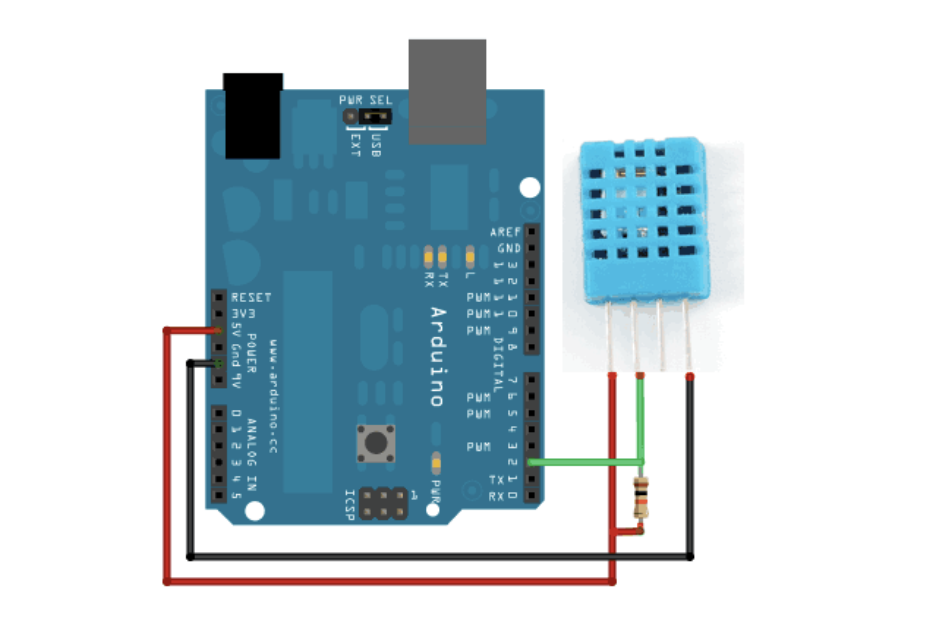
\includegraphics[width=12cm, height=6cm]{ESP32/AM2302.png}
		\caption{AM2302} 
		\label{fig:Python 3.10.}
	\end{center}
\end{figure}	

\subsection{Functions}
The DHT22 \cite{Taghoy:2018}, also known as AM2302, is a widely used sensor for measuring temperature and humidity in various applications. Below are the detailed functions and capabilities of the DHT22 sensor:

\begin{itemize}
	\item Temperature Measurement
	\begin{itemize}
		\item Function: The primary function of the DHT22 sensor is to measure the ambient temperature.
		\item Range: It can measure temperatures from -40°C to 80°C (-40°F to 176°F).
		\item Accuracy: The sensor offers an accuracy of ±0.5°C, making it suitable for applications requiring precise temperature readings.
		\item Resolution: The temperature is reported with a resolution of 0.1°C, which allows for fine-grained monitoring of temperature changes.
		\item Output: The temperature data is provided as a digital signal, which can be easily read and processed by microcontrollers like the ESP32 Nano.
	\end{itemize}
	\item Humidity Measurement
	\begin{itemize}
		\item Function: The DHT22 also measures the relative humidity of the surrounding air.
		\item Range: The sensor can measure humidity levels from 0% to 100% relative humidity (RH).
		\item Accuracy: It has a humidity accuracy of ±2 to ±5 RH, depending on the specific humidity range, which is sufficient for most general-purpose applications.
		
		\item Resolution: The humidity readings have a resolution of 0.1 RH, enabling detailed monitoring of humidity variation
		\item Output: Humidity data is provided as a digital signal, compatible with microcontrollers for easy data acquisition and analysis.

	\end{itemize}
\end{itemize}


\subsection{Example - Manual}

Here’s an example sketch that shows how to use the DHT sensor library to read temperature and humidity data from a DHT22 sensor:


	\begin{Arduino}
	#include "DHT.h"
	
	#define DHTPIN 2      // Digital pin connected to the DHT sensor
	#define DHTTYPE DHT22 // DHT22 (AM2302)
	
	DHT dht(DHTPIN, DHTTYPE);
	
	void setup() {
		Serial.begin(115200);
		Serial.println(F("DHT22 sensor test!"));
		
		dht.begin();
	}
	
	void loop() {
		delay(2000); // Wait a few seconds between measurements.
		
		// Reading temperature or humidity takes about 250 milliseconds!
		float h = dht.readHumidity();
		// Read temperature as Celsius (the default)
		float t = dht.readTemperature();
		// Read temperature as Fahrenheit (isFahrenheit = true)
		float f = dht.readTemperature(true);
		
		// Check if any reads failed and exit early (to try again).
		if (isnan(h) || isnan(t) || isnan(f)) {
			Serial.println(F("Failed to read from DHT sensor!"));
			return;
		}
		
		// Compute heat index in Fahrenheit (the default)
		float hif = dht.computeHeatIndex(f, h);
		// Compute heat index in Celsius (isFahreheit = false)
		float hic = dht.computeHeatIndex(t, h, false);
		
		Serial.print(F("Humidity: "));
		Serial.print(h);
		Serial.print(F("%  Temperature: "));
		Serial.print(t);
		Serial.print(F("C "));
		Serial.print(f);
		Serial.print(F("F  Heat index: "));
		Serial.print(hic);
		Serial.print(F("C "));
		Serial.print(hif);
		Serial.println(F("F"));
	}
	
	\end{Arduino}
	
	

	

\subsection{Example}

measuring temperature and humidity in various IoT projects. It provides accurate readings with good precision and reliability. Here are some examples of using the DHT22 sensor with the ESP32 Nano, including the circuit connections and example code:

\textbf{Example:} Reading Temperature and Humidity Using DHT22 with ESP32 Nano


\textbf{Components Needed:}
\begin{itemize}
	\item ESP32 Nano development board
	\item DHT22 (AM2302) temperature and humidity sensor
	\item Breadboard and jumper wires
	\item 10k ohm resistor (optional for pull-up)
\end{itemize}
	



\subsection{Example - Code}

\textbf{Requirements:} 

\begin{itemize}
	\item Arduino board 
	\item DHT22 sensor
	\item 10k ohm pull-up resistor
	\item DHT library by Adafruit (can be installed via Arduino IDE Library Manager)
\end{itemize}


\textbf{Circuit:} 


\begin{enumerate}
	\item Connect the VCC pin of the DHT22 sensor to the 5V pin of the Arduino.
	\item Connect the GND pin of the DHT22 sensor to the GND pin of the Arduino.
	\item Connect the DATA pin of the DHT22 sensor to digital pin 2 of the Arduino.
	\item Place a 10k ohm pull-up resistor between the DATA pin and VCC pin.
\end{enumerate}

\begin{Arduino}
	#include "DHT.h"
	
	// Define the pin where the DHT22 sensor is connected
	#define DHTPIN 2
	
	// Define the type of sensor used: DHT22 (AM2302)
	#define DHTTYPE DHT22
	
	// Initialize DHT sensor
	DHT dht(DHTPIN, DHTTYPE);
	
	void setup() {
		// Start serial communication at 9600 baud rate
		Serial.begin(9600);
		Serial.println("DHT22 Sensor Example");
		
		// Initialize the DHT sensor
		dht.begin();
	}
	
	void loop() {
		// Wait a few seconds between measurements
		delay(2000);
		
		// Read humidity and temperature as floating-point numbers
		float humidity = dht.readHumidity();
		float temperatureC = dht.readTemperature(); // Temperature in Celsius
		float temperatureF = dht.readTemperature(true); // Temperature in Fahrenheit
		
		// Check if any readings failed and exit early (to try again)
		if (isnan(humidity) || isnan(temperatureC) || isnan(temperatureF)) {
			Serial.println("Failed to read from DHT sensor!");
			return;
		}
		
		// Compute heat index in Fahrenheit (the default)
		float heatIndexF = dht.computeHeatIndex(temperatureF, humidity);
		
		// Compute heat index in Celsius
		float heatIndexC = dht.computeHeatIndex(temperatureC, humidity, false);
		
		// Print the results to the serial monitor
		Serial.print("Humidity: ");
		Serial.print(humidity);
		Serial.print(" %\t");
		Serial.print("Temperature: ");
		Serial.print(temperatureC);
		Serial.print(" C ");
		Serial.print(temperatureF);
		Serial.print(" F\t");
		Serial.print("Heat index: ");
		Serial.print(heatIndexC);
		Serial.print(" C ");
		Serial.print(heatIndexF);
		Serial.println(" F");
	}
	
	
\end{Arduino}



\subsection{Example - Files}



\subsection{Calibration}

cite method

\subsection{Simple Code}

In the sketch \ref{Nano:PowerLEDTest}, a variable is connected to pin 25.\index{Pin!Pin 25} The pin 25 is defined as an output in the function \PYTHON{setup}. In the function \PYTHON{loop}, the \ac{led} is switched on for 1 second and switched off for 1 second so that the \ac{led} flashes accordingly.



{
	\captionof{code}{Simple sketch to control the power LED}\label{Nano:PowerLEDTest}
	\ArduinoExternal{}{../../Code/Nano33BLESense/Test/TestLEDPower.ino}
}

\bigskip

This is just a simple example. The variable \PYTHON{LED\_PWR} is already defined, so the assignment is not necessary. The command \PYTHON{delay} should be avoided in an Arduino sketch. Instead, variables of the type \PYTHON{elapsedMillis} should be used.


\subsection{Simple Application}



\subsection{Tests}

\subsection{Simple Function Test}

The simplest test is the flashing of the \ac{led} at 2 Hz.

{
	\captionof{code}{Simple sketch to test the power LED}\label{Nano:PowerLEDTest}
	\ArduinoExternal{}{../../Code/Nano33BLESense/Test/TestLEDPower.ino}
}


\subsection{Test all Functions}

The brightness of the power LED can be controlled. This is demonstrated in the example sketch \ref{Nano:PowerLEDTestPWM}.

Using the pulse width modulation, the brightness is gradually increased to the maximum value and then gradually reduced to 0 again.




{
	\captionof{code}{Simple sketch to check the battery state using the power LED}\label{Nano:PowerLEDTestPWM}
	\ArduinoExternal{}{../../Code/Nano33BLESense/Test/TestLEDPowerBrightness.ino}
}

\section{Light Sensors}
\subsection{Light Sensors [BH1750]}

The performance of indoor illumination control in many applications, such as in an intelligent building, relies on the quality of the light sensors. In many cases, the light level is not uniform and depends on the direction of the illumination source. It usually requires multiple sensors set up in different directions to gather the overall light level. We propose a system that can provide multi-directional light sensing data by rotating a single sensor. This approach overcomes the problem of static sensors network by dynamically changing the measuring angular of the light sensor. We present a sensor system prototype using the ESP8266 controller board, BH1750 light sensor, stepper motor, and 3D printed rotation base mechanism. The system can calculate the sensing angle and transmit sensing data to the monitoring unit or Internet of Things platforms for visualization and analysis. The testing results in normal workrooms show that the  rotating sensor can measure the light level in different directions and detect the direction of the main illumination s  ource. Even blocking some directions, the sensor still is able to accurately measure and provide sensing information on the remaining directions. Our sensor system is useful in both whole lighting and local lighting control applications.

The BH1750 is a 16-bit ambient light sensor that communicates via I2C protocol. It outputs luminosity measurements in lux (SI-derived unit of illuminance). It can measure a minimum of 1 lux and a maximum of 65535 lux. The sensor may come in different breakout board formats. See pictures below. Both images represent a BH1750 sensor.

\begin{itemize}
	\item[\checkmark] The sensor provides a direct digital output in lux, simplifying the data processing compared to analog sensors.
	\item[\checkmark] It can measure light intensity from 1 to 65535 lux, making it suitable for a variety of lighting conditions.
	\item[\checkmark] With a current consumption of just a few microamps in low power mode, it is ideal for battery-powered applications.
	\item[\checkmark] The BH1750 communicates via the I2C bus, allowing easy integration with microcontrollers like the ESP32.
\end{itemize}

\subsection{Specification}
\subsection{Light Sensors [BH1750]}

\textbf{(1) High Precision:} 
The BH1750 offers high precision in light measurement with a wide range of 1 to 65535 lux, making it suitable for various lighting conditions from very low light to \cite{Gao:2017} bright sunlight.\\ \\

\textbf{(2) Low Power Consumption:} \\
With a typical current  of 0.12 mA, it is ideal for battery-powered devices. The sensor also has a very low standby current of 0.01 μA, ensuring minimal power usage when not actively measuring light. The BH1750 communicates via the I²C bus, which is a standard interface used in many microcontrollers. This makes it easy to integrate with other devices and allows for up to 400 kHz communication speed \cite{Gupta:2024}.

\begin{center} % Center the table
	\begin{tabular}{|l|l|} % Specify alignment and vertical lines
		\hline % Top horizontal line
		\textbf{Model} & \textbf{BH1750} \\
		\hline % Horizontal line
		Supply Voltage & (VCC): 2.4V to 3.6V \\
		\hline
		Output signal & Digital 16-bit serial \\
		\hline
		Communication & I²C bus \\
		\hline
		Temperature & -40C to +85C  \\
		\hline
		Accuracy & ±20 (under certain conditions)  \\
		\hline
		Resolution or sensitivity & (H-Resolution Mode): 120 ms \\
		
		\hline % Bottom horizontal line
	\end{tabular}
\end{center}

\begin{itemize}
	\item cite data sheet
	\item Circuit Diagram
\end{itemize}

\subsection{Bibliothek}

The sensor can measure in 3 different qualities: one low quality mode and two high quality modes.
To enhance the range, the sampling time is adjustable from 31 to 254.
However, this is not a measuring time in seconds or milliseconds, but it is called Measurement Time Register = MTreg. At auto ranging you can read more about \cite{Xiangyan:2020} MTreg hp_BH1750.



\subsection{Description}
Using the BH1750 with Arduino is a simple matter of wiring up the sensor to your Arduino-compatible microcontroller, installing the hp_BH1750 library written by Stefan Armborst, and running one of many very well written examples. Usually we write our own library but we were so impressed by Stefan's that we didn't think we could possibly improve on it \cite{Muhammad:2020} , so use it!

\subsection{Installation}
This wiring if you want to connect via I2C interface. The I2C address address for the BH1750 is 0x23 and can be switched to 0x5C by pulling the address pin high to VCC

Here is how to wire up the sensor using one of the STEMMA QT connectors. The examples show a Metro but wiring will work the same for an Arduino or other compatible board.
\\
We will need :

\begin{enumerate}
	\item Arduino Board" Uno,Nano,mini 
	\item BH1750 Breakout .
	\item Solderless Jumper
	\item CD4050 Hex Buffer IC , Or 510 Ohm resistor *3
\end{enumerate}

Here is how to wire the sensor to a board using a solderless breadboard:
\begin{enumerate}
	\item Connect board VIN (red wire) to Arduino 5V if you are running a 5V board Arduino (Uno, etc.). If your board is 3V, connect to that instead.
	\item Connect board GND (black wire) to Arduino GND
	\item Connect board SCL (yellow wire) to Arduino SCL
	\item Connect board SDA (blue wire) to Arduino SDA
\end{enumerate}




Luckily it is trivial to connect to these sensors, they have fairly long 0.1"-pitch pins so you can plug them into any breadboard, perfboard or similar.

in Newest  Arduino Board "Like Arduino R3" Has I/OREF Pin above reset Pin , his pin on the Arduino board provides the voltage reference with which the microcontroller operates. A properly configured shield can read the IOREF pin voltage and select the appropriate power source or enable voltage translators on the outputs for working with the 5V or 3.3V.  very nice you can use it. About ADDR Pin , I prepare a Library " I will talk about in the next step " , You can select the address of your breakout , Even 0x23 \cite{Cihan:2020} , or 0X5C , this action depend on the ADDR Pin status , if connecting to Gnd , the address will be 0x23 , else if ADDR Connecting to Vcc The address will be 0X5C  .
 \\

This diagram shows how we will connect for the testing sketch. Connect data to pin 2, you can change it later to any pin.

\begin{figure}  
	\begin{center}
		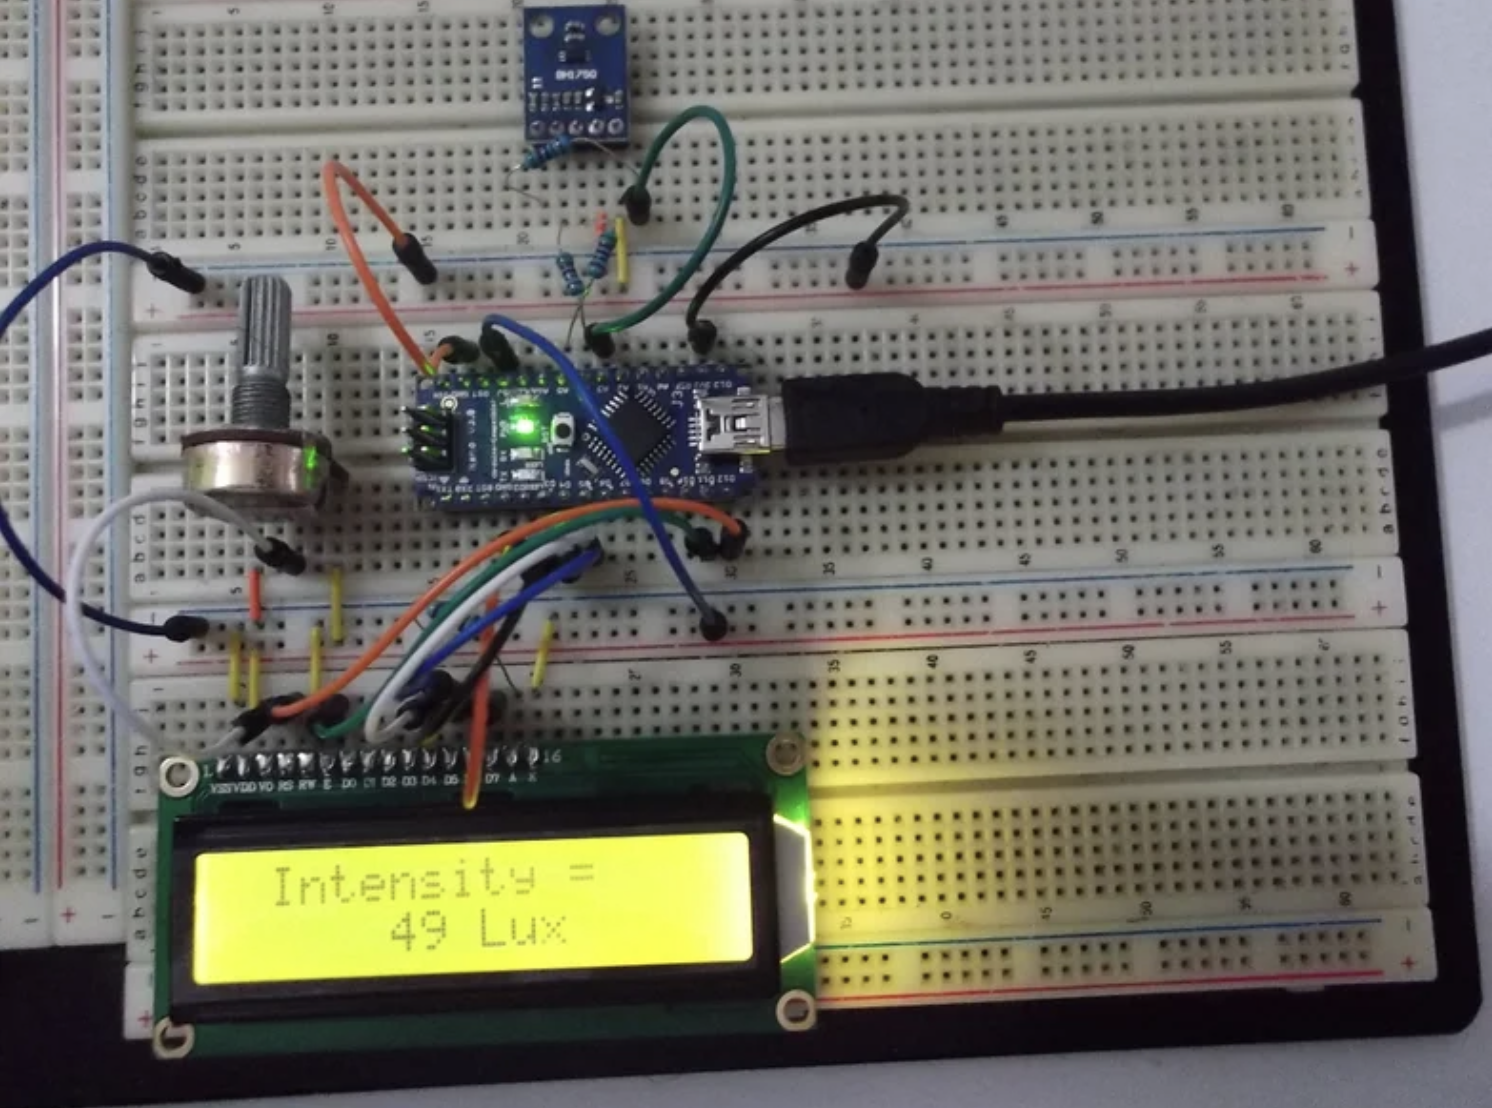
\includegraphics[width=12cm, height=6cm]{ESP32/LCD_1602_and_BH1750.png}
		\caption{LCD_1602_and_BH1750} 
		\label{fig:Python 3.10.}
	\end{center}
\end{figure}	



\begin{figure}  
	\begin{center}
		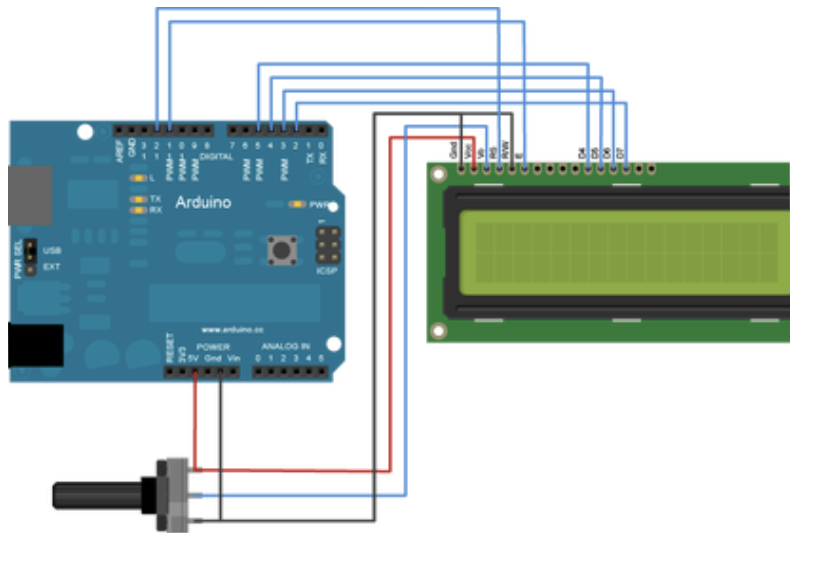
\includegraphics[width=12cm, height=6cm]{ESP32/LightSensor.png}
		\caption{Light Sensor} 
		\label{fig:Python 3.10.}
	\end{center}
\end{figure}	

\subsection{Functions}
The BH1750 is a digital light sensor IC that measures ambient light intensity. It communicates with a microcontroller via the I2C bus and provides a wide range \cite{Podbucki:2023} of illuminance values. Here's a detailed description of its functions:

\begin{itemize}
	\item Ambient Light Measurement:
	\begin{itemize}
		\item The primary function of the BH1750 is to measure the intensity of ambient light. It converts light intensity into a digital signal that can be read by a microcontroller.
		\item The measurement range is typically from 1 to 65535 lux, allowing it to handle very dim to very bright light conditions.
	\end{itemize}
	\item I2C Interface:
	\begin{itemize}
		\item The BH1750 uses the I2C protocol for communication, making it easy to integrate with microcontrollers and other devices.
		\item It has two I2C addresses (0x23 and 0x5C), selectable via address pin configuration.
	\end{itemize}
	
		\item Automatic Gain Control:
	\begin{itemize}
		\item The BH1750 adjusts its sensitivity automatically based on the ambient light conditions, ensuring accurate readings across its full measurement range.
	\end{itemize}
	
		\item Calibration and Accuracy:
	\begin{itemize}
		\item The sensor is factory-calibrated to ensure high accuracy and stability over time and varying conditions.
		\item Typical accuracy is within ±20 of the measured value.
	\end{itemize}
\end{itemize}


\subsection{Example - Manual}

Convert the two bytes of data into a lux value using the formula provided in the datasheet \cite{Dewi:2022}.


\begin{Arduino}
	#include <Wire.h>
	
	#define BH1750_ADDRESS 0x23 // I2C address
	
	void setup() {
		Wire.begin();
		Serial.begin(9600);
		configureBH1750();
	}
	
	void loop() {
		uint16_t lux = readBH1750();
		Serial.print("Light Intensity: ");
		Serial.print(lux);
		Serial.println(" lx");
		delay(1000);
	}
	
	void configureBH1750() {
		Wire.beginTransmission(BH1750_ADDRESS);
		Wire.write(0x10); // Send high-resolution mode command
		Wire.endTransmission();
	}
	
	uint16_t readBH1750() {
		Wire.beginTransmission(BH1750_ADDRESS);
		Wire.requestFrom(BH1750_ADDRESS, 2);
		while (Wire.available() < 2);
		uint16_t lux = Wire.read();
		lux <<= 8;
		lux |= Wire.read();
		return lux / 1.2; // Convert to lux
	}
	
	
\end{Arduino}





\subsection{Example}

The BH1750 is a reliable and easy-to-use light sensor for various applications. With its I2C interface and different measurement modes, it provides accurate ambient light measurements suitable for smart devices, lighting systems

\textbf{Example:} \cite{Suryana:2020}Continuously reads the light intensity in lux from the BH1750 sensor and prints it to the serial monitor every second.


\textbf{Components Needed:}
\begin{itemize}
	\item ESP32 Nano development board
	\item DHT22 (AM2302) temperature and humidity sensor
	\item Breadboard and jumper wires
	\item 10k ohm resistor (optional for pull-up)
\end{itemize}




\subsection{Example - Code}

\textbf{Connect the BH1750 sensor to the Arduino as follows::} 

\begin{itemize}
	\item VCC to 3.3V or 5V on Arduino
	\item GND to GND on Arduino
	\item SCL to A5 on Arduino (or the dedicated I2C SCL pin)
	\item SDA to A4 on Arduino (or the dedicated I2C SDA pin)
	\item ADDR to GND (for I2C address 0x23)
\end{itemize}



\begin{Arduino}
	#include <Wire.h>
	
	#define BH1750_ADDRESS 0x23 // I2C address when ADDR is connected to GND
	
	void setup() {
		Wire.begin(); // Initialize I2C
		Serial.begin(9600); // Initialize serial communication
		configureBH1750(); // Configure BH1750 sensor
	}
	
	void loop() {
		uint16_t lux = readBH1750(); // Read light level
		Serial.print("Light: ");
		Serial.print(lux);
		Serial.println(" lx");
		delay(1000); // Wait for 1 second
	}
	
	void configureBH1750() {
		Wire.beginTransmission(BH1750_ADDRESS);
		Wire.write(0x10); // Send continuous high-resolution mode command
		Wire.endTransmission();
	}
	
	uint16_t readBH1750() {
		uint16_t lux = 0;
		Wire.beginTransmission(BH1750_ADDRESS);
		Wire.requestFrom(BH1750_ADDRESS, 2); // Request 2 bytes from BH1750
		
		if (Wire.available() == 2) { // Wait for data to become available
			lux = Wire.read(); // Read the high byte
			lux <<= 8; // Shift high byte to high position
			lux |= Wire.read(); // Read the low byte and combine with high byte
		}
		
		return lux / 1.2; // Convert raw value to lux (assuming high-resolution mode)
	}
	
	
	
\end{Arduino}



\subsection{Example - Files}



\subsection{Calibration}

Calibration involves comparing the BH1750's readings with a known reference light meter under controlled lighting conditions and adjusting the readings accordingly.

Here’s a step-by-step guide to calibrate the BH1750:
cite method

\subsection{Simple Code}

In the sketch \ref{Nano:PowerLEDTest}, a variable is connected to pin 25.\index{Pin!Pin 25} The pin 25 is defined as an output in the function \PYTHON{setup}. In the function \PYTHON{loop}, the \ac{led} is switched on for 1 second and switched off for 1 second \cite{Lijun:201} so that the \ac{led} flashes accordingly.



{
	\captionof{code}{Simple sketch to control the power LED}\label{Nano:PowerLEDTest}
	\ArduinoExternal{}{../../Code/Nano33BLESense/Test/TestLEDPower.ino}
}

\bigskip

This is just a simple example. The variable \PYTHON{LED\_PWR} is already defined, so the assignment is not necessary. The command \PYTHON{delay} should be avoided in an Arduino sketch. Instead, variables of the type \PYTHON{elapsedMillis} should be used.


\subsection{Simple Application}



\subsection{Tests}

\subsection{Simple Function Test}

The simplest test is the flashing of the \ac{led} at 2 Hz.

{
	\captionof{code}{Simple sketch to test the power LED}\label{Nano:PowerLEDTest}
	\ArduinoExternal{}{../../Code/Nano33BLESense/Test/TestLEDPower.ino}
}


\subsection{Test all Functions}

The brightness of the power LED can be controlled. This is demonstrated in the example sketch \ref{Nano:PowerLEDTestPWM}.

Using the pulse width modulation, the brightness is gradually increased to the maximum value and then gradually reduced to 0 again.




{
	\captionof{code}{Simple sketch to check the battery state using the power LED}\label{Nano:PowerLEDTestPWM}
	\ArduinoExternal{}{../../Code/Nano33BLESense/Test/TestLEDPowerBrightness.ino}
}

\subsection{Simple Application}


There are different situations where it might be useful to program the power LED of the Arduino Nano. For example, you could use it to:

\begin{itemize}
	\item Indicate the status of the board, such as whether it is connected to a power source, a computer, or a sensor.
	\item  Display the battery level of the board, by changing the brightness or color of the power \ac{led}.
	\item Create a visual alarm or notification, by making the power LED blink or flash in a certain pattern.
\end{itemize}

\bigskip

A simple application is to check the condition of the battery. The sktech \ref{Nano:PowerLEDTestBattery} demonstrates, if the voltage drops too low, the power LED flashes.

{
	\captionof{code}{Simple sketch to check the battery state using the power LED}\label{Nano:PowerLEDTestBattery}
	\ArduinoExternal{}{../../Code/Nano33BLESense/Test/TestLEDPowerBattery.ino}
}

\section{Touch Sensor}
\subsection{Touch Sensor}

The ESP32 touch pins can sense variations in anything that holds an electrical charge. They are often used to wake up the ESP32 from deep sleep. The ESP32 has 10 capacitive touch GPIOs. These GPIOs can sense variations in anything that holds an electrical charge, like the human skin. So they can detect variations induced when touching the GPIOs with a finger \cite{Azzam:2021}.

A touch sensor system is built on a substrate which carries electrodes and relevant connections under a protective flat surface. When the surface is touched, the capacitance variation is used to evaluate if the touch was valid.

The sensing pads can be arranged in different combinations (e.g., matrix, slider), so that a larger area or more points can be detected. The touch pad sensing process is under the control of a hardware-implemented finite-state machine (FSM) which is initiated by software \cite{Arif:202} or a dedicated hardware timer.

For design, operation, and control registers of a touch sensor, see ESP32 Technical Reference Manual > On-Chip Sensors and Analog Signal Processing.



\subsection{Specification}
\subsection{Touch Sensor }

Touch sensor is a peripheral, that has an internal oscilator circuit and it measures charge/discharge frequency over a fixed period of time on respective GPIO pins. Therefore these touch sensors are also known as capacitive sensors. For example, if you touch any of these pins, finger electrical charge will change this number of cycles, by changing the RC circuit attached to the touch sensor \cite{Arif:2023}. The TouchRead() will return the number of cycles (charges/discharges) in a certain time (meas). The change of this count will be used to validate if a touch has happened or not. These pins can be easily integrated into capacitive pads, and replace mechanical buttons \cite{Kumar:2024}.



\begin{itemize}
	\item Protective Cover
	Protective cover refers to the touch panel. The touch panel must be of insulating material that helps isolate and protect the touch electrode from the outside. However, the protective cover reduces the touch sensitivity. Therefore, the overlay's thickness and material should be selected depending on the specific usage scenarios to provide both required protection and sensitivity \cite{Rajalakshmi:2017}.
	\item Touch Electrode
	The touch electrode is a key part of a touch sensor system. When a finger touch takes place, a plate capacitor that is in parallel to the electrode will be formed, and the capacitance on the touch channel changes accordingly. The touch electrode must be conductive. A touch electrode can be copper foil on a PCB, a metal plate, a touch spring, etc.
	\item Insulation Substrate
	The non-conductive substrate provides support to the touch electrodes.
	
	\itemTraces The traces connect the touch electrode and the chip, including PCB traces and connectors. Poor trace routing is very likely to introduce interferences and parasitic capacitance.
\end{itemize}

\begin{center} % Center the table
	\begin{tabular}{|l|l|} % Specify alignment and vertical lines
		\hline % Top horizontal line
		\textbf{Capacitance composition} & \textbf{Description} \\
		\hline % Horizontal line
		Cgrounde & Capacitance between the circuit ground and the earth \\
		\hline
		Ccomponent & ESP32's intrinsic parasitic capacitance \\
		\hline
		Ctrace & Parasitic capacitance between the trace and the circuit ground \\
		\hline
		Celectrode & Parasitic capacitance between the touch electrode and the circuit ground  \\
		\hline
		Ctouch & Capacitance formed by a finger and the touch electrode relative to the earth  \\
		
		\hline % Bottom horizontal line
	\end{tabular}
\end{center}

\begin{figure}  
	\begin{center}
		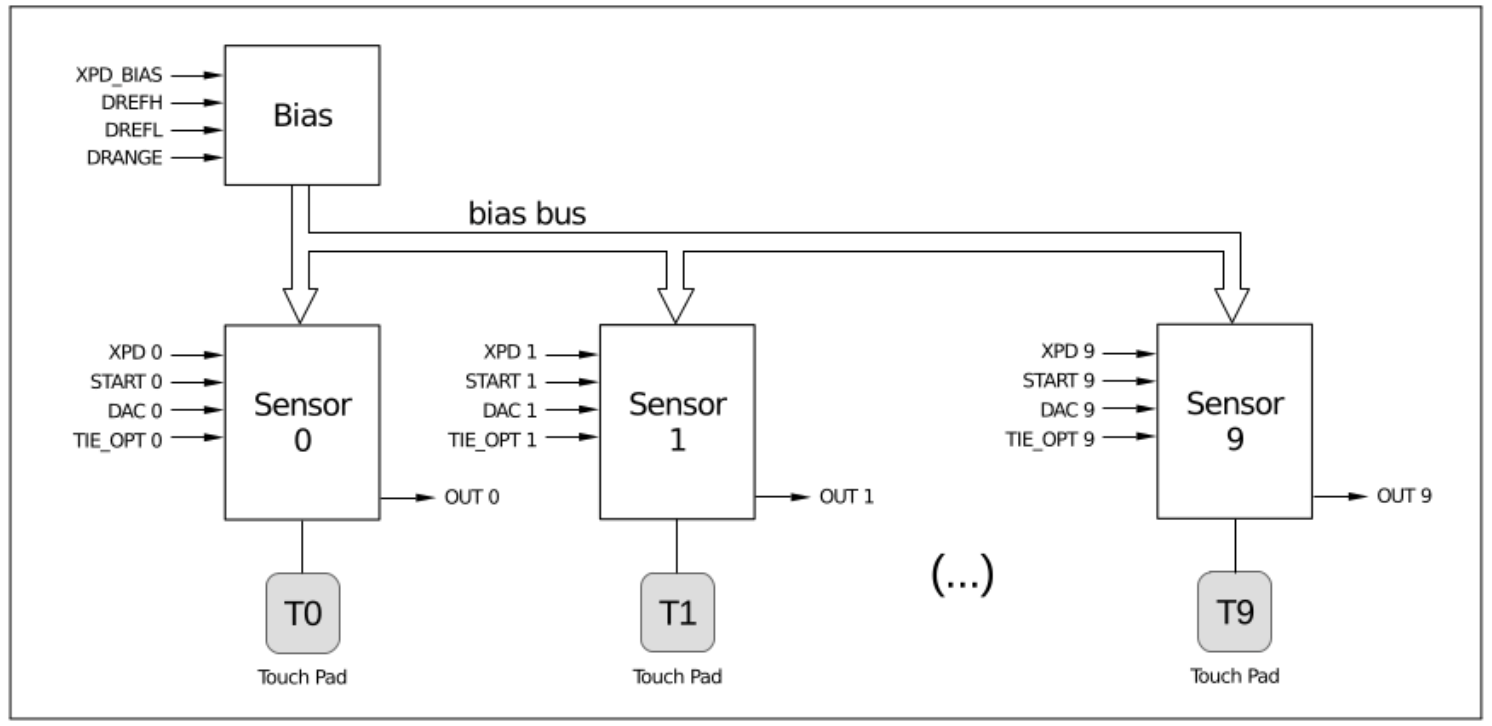
\includegraphics[width=12cm, height=6cm]{ESP32/Touch_Sensor_Internal_Structure.png}
		\caption{The internal structure of the touch sensor.} 
		\label{fig:Python 3.10.}
	\end{center}
\end{figure}	

\subsection{Bibliothek}

The sensor can measure in 3 different qualities: one low quality mode and two high quality modes.
To enhance the range, the sampling time is adjustable from 31 to 254.
However, this is not a measuring time in seconds or milliseconds, but it is called Measurement Time Register = MTreg. At auto ranging you can read more about \cite{Vogelgesang:2024} MTreg hp_BH1750.

\subsection{Description}
The ESP32 internal current source periodically charges and discharges each touch pin. During charge/discharge, the voltage at the touch pin swings from reference voltage high (drefH) to reference voltage low (drefL). As shown in the figure above, with the function of comparator, a charge/discharge cycle is counted after the charging from drefL to drefH and the discharging back to drefL is completed. During each swing, the touch sensor generates an output pulse (shown in the chart as ”OUT”) that will be counted \cite{Amin:2021}. The capacitance on the touch pin remains constant in an ideal environment without interferences. The number of output pulses (OUT) is constant over the same time interval.

The charge/discharge speed on the touch pin is determined by the strength of the output current from the internal current source. The current source strength is configured with register DAC[2:0]. drefH and drefL are set by registers DREFH[1:0] and DREFL[0], respectively \cite{Azzam:2021}.

When the finger touches the sensor, the parallel plate capacitor is formed between the finger and the sensor metal plate, and its equivalent capacitance is connected in parallel to the touch pin, increasing the capacitance on the touch pin. According to the formula du/dt = C/I, if the charge/discharge current remains the same and the capacitance increases, the charge/discharge time will increase, and the output pulse count (OUT) will decrease during the same time interval. By comparing the difference between the output pulse counts during the same time interval, we can conclude whether the touch pad has been touched \cite{Arif:2023}.

At the application level, the user can call the API function touch_pad_read (touch_pad_t touch_num, uint16_t * touch_value); to read the pulse counts (OUT).

\begin{figure}  
	\begin{center}
		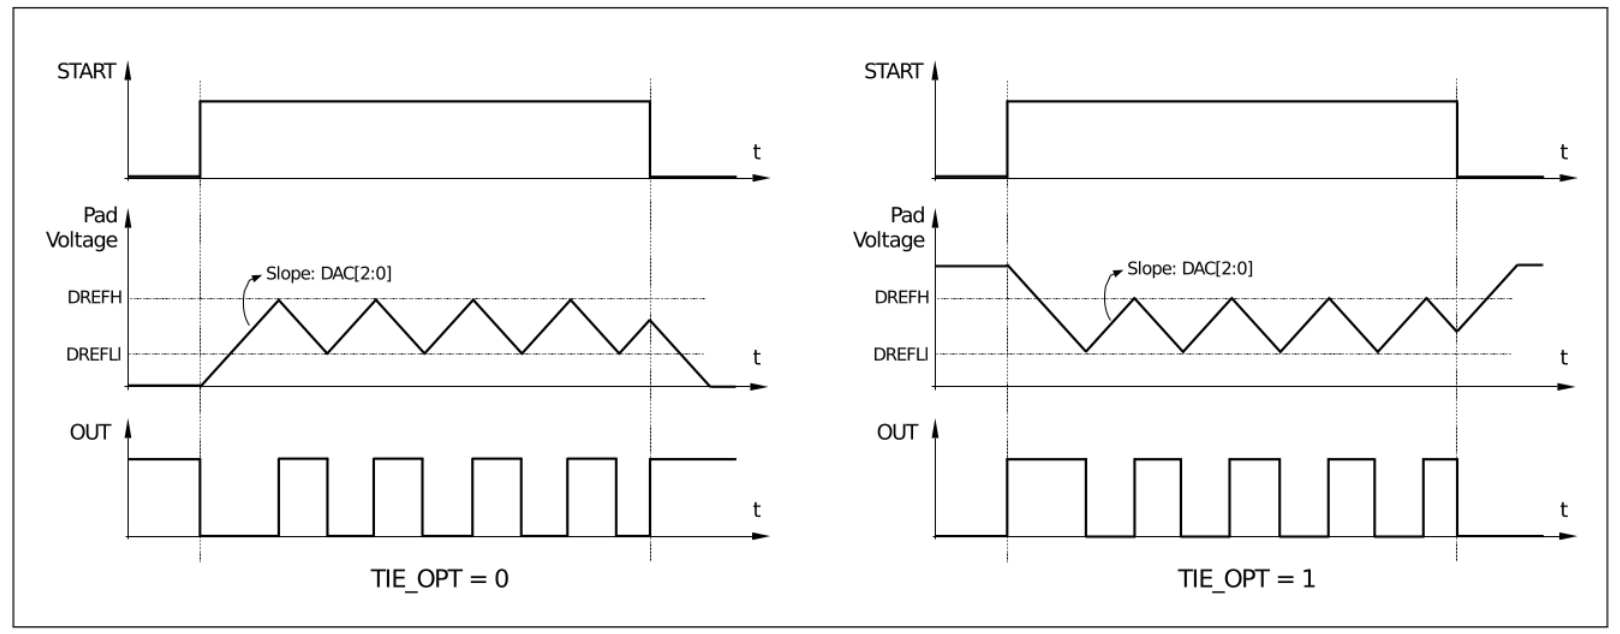
\includegraphics[width=12cm, height=6cm]{ESP32/Touch_Sensor_Operating_Flow.png}
		\caption{Touch Sensor Operating Flow} 
		\label{fig:Python 3.10.}
	\end{center}
\end{figure}	

\subsection{Installation}
The ESP32 microcontroller includes capacitive touch sensors that can be used to create touch-sensitive interfaces. Here’s a detailed guide on installing \cite{Vogelgesang:2024} and using the touch sensor capabilities of an ESP32:
\\
We will need :

\begin{enumerate}
	\item ESP32 development board
	\item Breadboard and jumper wires
	\item Capacitive touch pads (you can also use simple conductive materials like aluminum foil)
	\item Arduino IDE (or PlatformIO)
\end{enumerate}

Setting Up the Environment
\begin{enumerate}
	\item Install the Arduino IDE: If you don’t have it already, download and install the Arduino IDE from the Arduino.
	\item Add ESP32 Board Manager URL: Open the Arduino IDE, go to File -> Preferences, and in the "Additional Board Manager URLs" field:
	\item Install the ESP32 Board Package: Go to Tools -> Board -> Boards Manager, search for "ESP32", and install the package by Espressif Systems.
	\item Select the ESP32 Board: Go to Tools -> Board and select the appropriate ESP32 board model.
\end{enumerate}




Luckily it is trivial to connect to these sensors, they have fairly long 0.1"-pitch pins so you can plug them into any breadboard, perfboard or similar.

in Newest  Arduino Board "Like  R3" Has I/OREF Pin above reset Pin , his pin on the Arduino board provides the voltage reference with which the microcontroller operates. A properly configured shield can read the IOREF pin voltage and select the appropriate power source or enable voltage translators on the outputs for working with the 5V or 3.3V.  very nice you can use it. About ADDR Pin , I prepare a Library " I will talk about in the next step " , You can select the address of your breakout , Even 0x23 \cite{Cihan:2020} , or 0X5C , this action depend on the ADDR Pin status , if connecting to Gnd , the address will be 0x23 , else if ADDR Connecting to Vcc The address will be 0X5C  .
\\

This diagram shows how we will connect for the testing sketch. Connect data to pin 2, you can change it later to any pin.

\begin{figure}  
	\begin{center}
		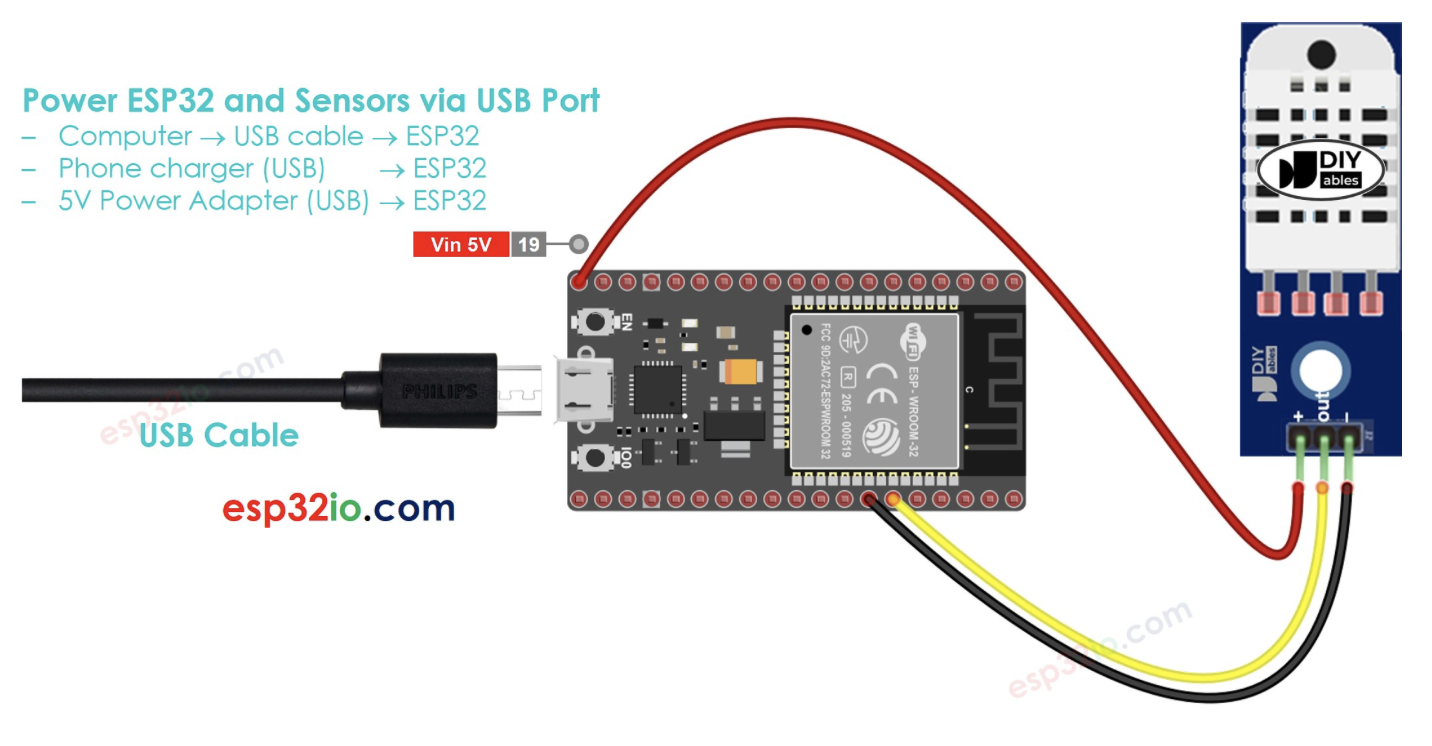
\includegraphics[width=12cm, height=6cm]{ESP32/installation_Touch_Sensor.png}
		\caption{Installation Touch Sensor} 
		\label{fig:Python 3.10.}
	\end{center}
\end{figure}	



\begin{figure}  
	\begin{center}
		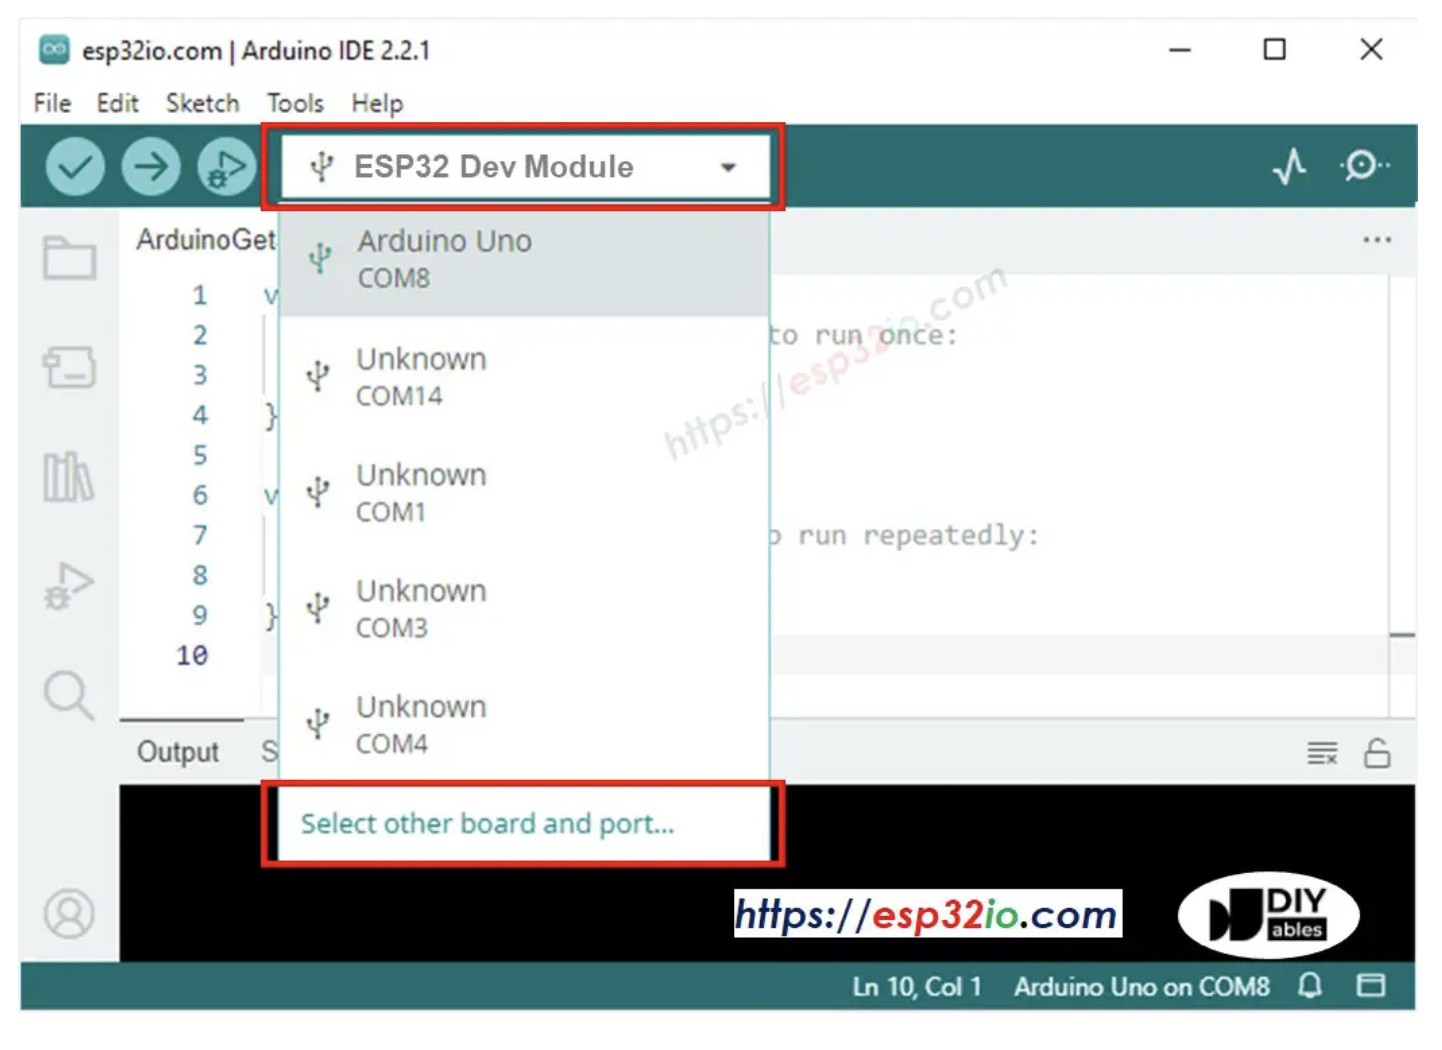
\includegraphics[width=12cm, height=6cm]{ESP32/installation_Touch_Sensor_2.png}
		\caption{Selection of esp32 board} 
		\label{fig:Python 3.10.}
	\end{center}
\end{figure}	

\subsection{Functions}
The ESP32 microcontroller has built-in capacitive touch sensor capabilities, allowing it to detect touch on designated GPIO pins. Here’s a detailed overview of the ESP32 touch sensor functions:

\begin{itemize}
	\item Initialization
	\begin{itemize}
		\item touchAttachInterrupt: This function attaches an interrupt to a touch pin. You can specify a callback function that gets executed when the touch value crosses a threshold.
		\item pin: The touch pin to attach the interrupt to.
		\item callback: The function to call when the interrupt is triggered.
		\item threshold: The threshold value for the touch sensor.
		\item touchRead: Reads the value from a specified touch pin. The value returned is an approximation of the capacitance of the touch pin.
	\end{itemize}
	\item Setting Touch Sensor Thresholds
	\begin{itemize}
		\item The BH1750 uses the I2C protocol for communication, making it easy to integrate with microcontrollers and other devices.
		\item It has two I2C addresses (0x23 and 0x5C), selectable via address pin configuration.
		\item pin: The touch pin to attach the interrupt to.
		\item pin: The touch pin to attach the interrupt to.
		\item pin: The touch pin to attach the interrupt to.
		\item pin: The touch pin to attach the interrupt to.
	\end{itemize}
	
	\item Setting Touch Sensor Thresholds
	\begin{itemize}
		\item The BH1750 adjusts its sensitivity automatically based on the ambient light conditions, ensuring accurate readings across its full measurement range.
	\end{itemize}
	
	\item Calibration and Accuracy:
	\begin{itemize}
		\item The sensor is factory-calibrated to ensure high accuracy and stability over time and varying conditions.
		\item Typical accuracy is within ±20 of the measured value.
	\end{itemize}
\end{itemize}


\subsection{Example - Manual}

This example creates a capacitive touch slider using multiple touch pins to detect the position of the touch.


\begin{Arduino}
	#include "driver/touch_pad.h"
	
	#define NUM_TOUCH_PINS 3
	const int touchPins[NUM_TOUCH_PINS] = {4, 13, 14};
	
	void setup() {
		Serial.begin(115200);
		for (int i = 0; i < NUM_TOUCH_PINS; i++) {
			touchAttachInterrupt(touchPins[i], onTouch, 40);
		}
	}
	
	void loop() {
		// Main loop does nothing, everything is handled by the interrupt
	}
	
	void onTouch() {
		for (int i = 0; i < NUM_TOUCH_PINS; i++) {
			if (touchRead(touchPins[i]) < 40) {
				Serial.print("Touched pin: ");
				Serial.println(touchPins[i]);
			}
		}
	}
	
	
	
\end{Arduino}





\subsection{Example}

This example detects the proximity of an object to the touch sensor..


\textbf{Components Needed:}
\begin{itemize}
	\item ESP32 Nano development board
	\item DHT22 (AM2302) temperature and humidity sensor
	\item Breadboard and jumper wires
	\item 10k ohm resistor (optional for pull-up)
\end{itemize}




\subsection{Example - Code}

\textbf{Connect the BH1750 sensor to the Arduino as follows::} 

\begin{itemize}
	\item VCC to 3.3V or 5V on Arduino
	\item GND to GND on Arduino
	\item SCL to A5 on Arduino (or the dedicated I2C SCL pin)
	\item SDA to A4 on Arduino (or the dedicated I2C SDA pin)
	\item ADDR to GND (for I2C address 0x23)
\end{itemize}



\begin{Arduino}
	#include "driver/touch_pad.h"
	
	#define TOUCH_PIN 4
	
	void setup() {
		Serial.begin(115200);
		touchAttachInterrupt(TOUCH_PIN, onProximity, 40);
	}
	
	void loop() {
		// Main loop does nothing, everything is handled by the interrupt
	}
	
	void onProximity() {
		Serial.println("Object is close!");
	}
	
\end{Arduino}



\subsection{Example - Files}



\subsection{Calibration}

Calibration involves comparing the BH1750's readings with a known reference light meter under controlled lighting conditions and adjusting the readings accordingly.

Here’s a step-by-step guide to calibrate the BH1750:
cite method

\subsection{Simple Code}
This example uses a touch sensor to control the brightness of an LED.

\begin{Arduino}
	#include "driver/touch_pad.h"
	
	#define TOUCH_PIN 4
	#define LED_PIN 2
	
	int brightness = 0;
	
	void setup() {
		Serial.begin(115200);
		pinMode(LED_PIN, OUTPUT);
		touchAttachInterrupt(TOUCH_PIN, onTouch, 40);
	}
	
	void loop() {
		analogWrite(LED_PIN, brightness);
	}
	
	void onTouch() {
		brightness = (brightness + 51) % 256;  // Increase brightness in steps of 20%
		Serial.print("Brightness: ");
		Serial.println(brightness);
	}
	
	
\end{Arduino}

\subsection{Simple Application}
This example implements debouncing for a touch sensor to avoid multiple triggers.

\begin{Arduino}
	#include "driver/touch_pad.h"
	
	#define TOUCH_PIN 4
	#define LED_PIN 2
	
	unsigned long lastTouchTime = 0;
	const unsigned long debounceDelay = 50;
	
	void setup() {
		Serial.begin(115200);
		pinMode(LED_PIN, OUTPUT);
		touchAttachInterrupt(TOUCH_PIN, onTouch, 40);
	}
	
	void loop() {
		// Main loop does nothing, everything is handled by the interrupt
	}
	
	void onTouch() {
		unsigned long currentTime = millis();
		if (currentTime - lastTouchTime > debounceDelay) {
			static bool ledState = false;
			ledState = !ledState;
			digitalWrite(LED_PIN, ledState ? HIGH : LOW);
			Serial.println("Touched!");
			lastTouchTime = currentTime;
		}
	}
	
	
	
\end{Arduino}




\subsection{Tests}

\subsection{Simple Function Test}

The simplest test is the flashing of the \ac{led} at 2 Hz.

{
	\captionof{code}{Simple sketch to test the power LED}\label{Nano:PowerLEDTest}
	\ArduinoExternal{}{../../Code/Nano33BLESense/Test/TestLEDPower.ino}
}


\subsection{Test all Functions}

The brightness of the power LED can be controlled. This is demonstrated in the example sketch \ref{Nano:PowerLEDTestPWM}.

Using the pulse width modulation, the brightness is gradually increased to the maximum value and then gradually reduced to 0 again.




{
	\captionof{code}{Simple sketch to check the battery state using the power LED}\label{Nano:PowerLEDTestPWM}
	\ArduinoExternal{}{../../Code/Nano33BLESense/Test/TestLEDPowerBrightness.ino}
}

\subsection{Simple Application}


There are different situations where it might be useful to program the power LED of the Arduino Nano. For example, you could use it to:

\begin{itemize}
	\item Indicate the status of the board, such as whether it is connected to a power source, a computer, or a sensor.
	\item  Display the battery level of the board, by changing the brightness or color of the power \ac{led}.
	\item Create a visual alarm or notification, by making the power LED blink or flash in a certain pattern.
\end{itemize}

\bigskip

A simple application is to check the condition of the battery. The sktech \ref{Nano:PowerLEDTestBattery} demonstrates, if the voltage drops too low, the power LED flashes.

{
	\captionof{code}{Simple sketch to check the battery state using the power LED}\label{Nano:PowerLEDTestBattery}
	\ArduinoExternal{}{../../Code/Nano33BLESense/Test/TestLEDPowerBattery.ino}
}

\section{Sound Sensors}
\subsection{Sound Sensors}

Sound sensors, often referred to as microphones, are devices that detect sound and convert it into an electrical signal. When used with an ESP32, a powerful microcontroller with built-in Wi-Fi and Bluetooth capabilities, sound sensors can enable various applications such as voice recognition, ambient noise monitoring, and smart home automation.

The working of the sounds sensor module is very simple, the main component in this module is a condenser microphone. The microphone gives out only analog signals when a sound wave hits the diaphragm of the sensor. This analog signal gets processed by the op-amp and we get the digital output. The main component of a sound sensor is a microphone. There are many different types of microphones, like Carbon Microphones, Fiber Optic Microphones, Ribbon Microphones, and Laser Microphones, but the sound sensor module we are using has a condenser microphone. An image of the sound sensor module is shown below. a condenser microphone consists of two charged metal plates. The first plate is called the diaphragm and the second plate is the backplate of the microphone. These two plates together form a capacitor. When a sound wave hits the diaphragm of the microphone the diaphragm starts to vibrate, and the distance between the two plates changes. The movement of the diaphragm and the change in spacing produces the electrical signal that corresponds to the sound picked up by the microphone and this signal then gets processed by the onboard op-amp. This module also has two built-in onboard LEDs, one of which lights up when power is applied to the board and the other one lights up when the incoming audio signal exceeds the threshold value set by the potentiometer.



\subsection{Specification}
\subsection{Sound Sensors}

In the schematic, we have an LM393 op-amp that is a low-power, low-cost, low-offset voltage op-amp that can be powered from a 3.3V or 5V supply. Please note that the analog output voltage of the device will depend on the supply voltage of the device. The main job of this op-amp is to convert the incoming analog signal from the sensor probe to a digital signal. There is also this 10K potentiometer that is used to set a reference voltage for the op-amp, also this potentiometer is used to generate the reference voltage for the analog out function of the module.

If the input voltage of the sensor goes below the threshold voltage set by the potentiometer, the output of the op-map goes low. Other than that we have two LEDs. The first one is a power LED and the other one is the trigger LED. The power LED turns on when power is applied to the board and the trigger LED turns on when a certain set threshold is reached. This is how this basic circuit works.

\begin{figure}  
	\begin{center}
		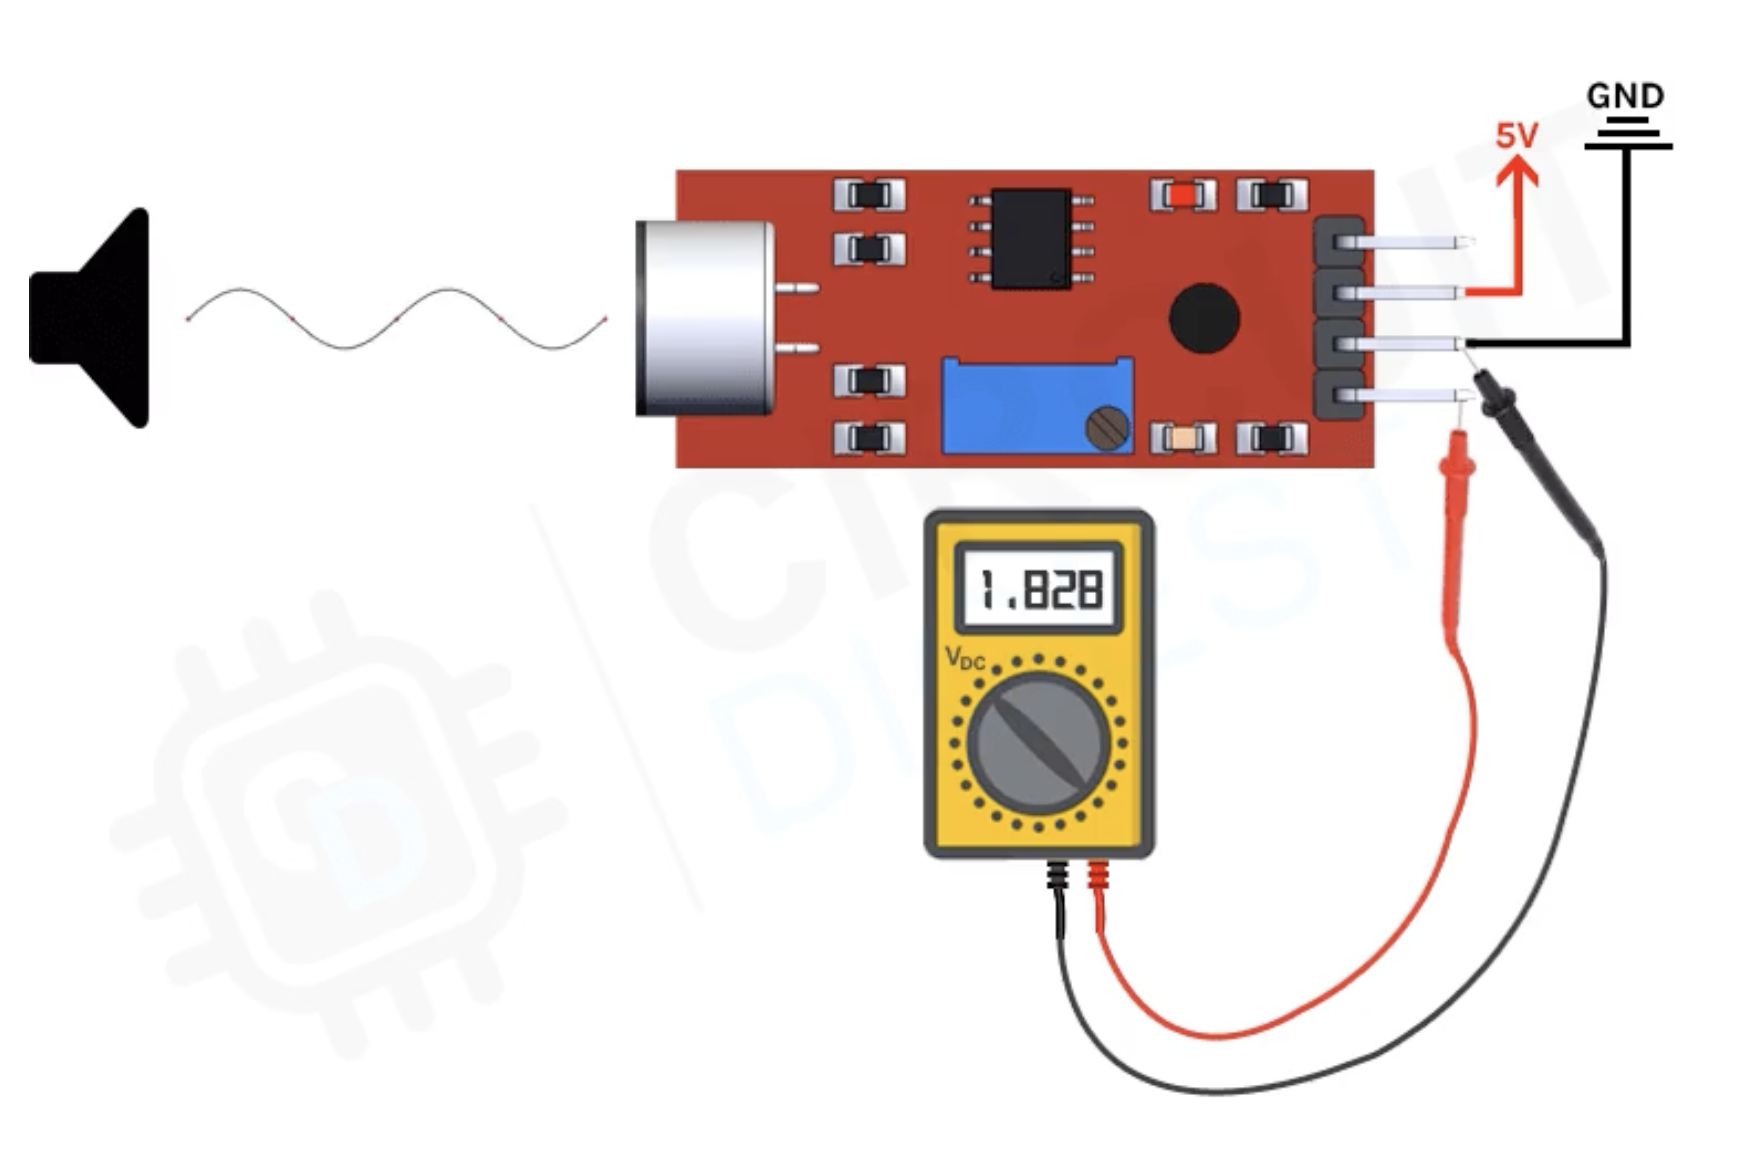
\includegraphics[width=12cm, height=6cm]{ESP32/sound_sendor_Img.png}
		\caption{Sound sensor with Arduino.} 
		\label{fig:Python 3.10.}
	\end{center}
\end{figure}	


Types of Sound Sensors
\begin{itemize}
	\item Electret Microphone:
	A small and cost-effective microphone that uses a permanently charged material (electret) to convert sound into an electrical signal.
	
	\item MEMS Microphone
	A Micro-Electro-Mechanical System microphone, which is smaller and more robust compared to electret microphones, often providing better performance and digital output.
	
	\item Working Principle
	Sound sensors typically consist of a microphone element that detects sound waves and converts them into an electrical signal. This signal is then amplified and processed to be read by a microcontroller like the ESP32.
\end{itemize}



\begin{figure}  
	\begin{center}
		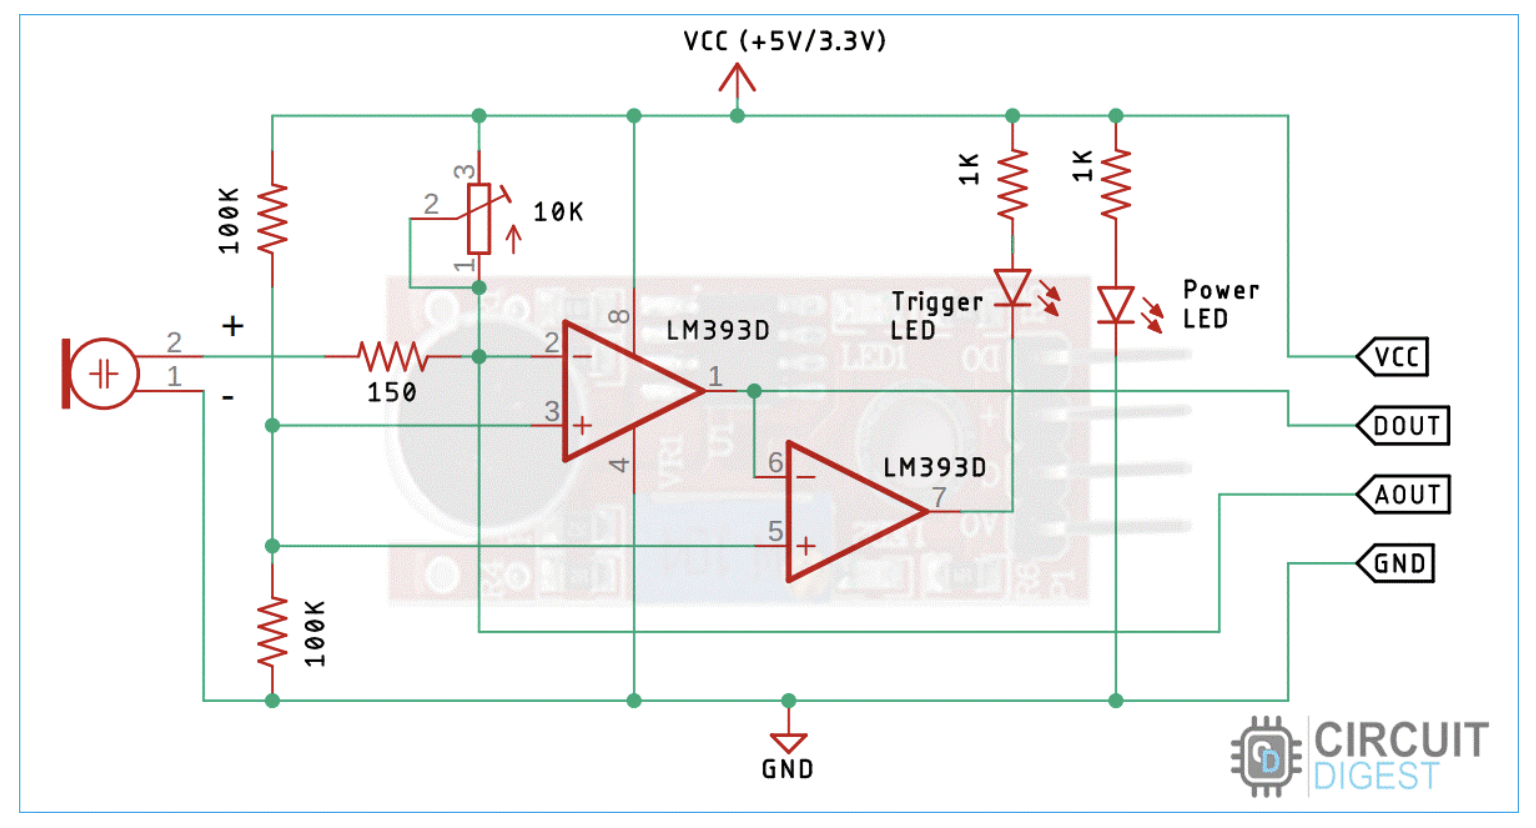
\includegraphics[width=12cm, height=6cm]{ESP32/sound_sensor_working_system.png}
		\caption{Sound Sensor Working System.} 
		\label{fig:Python 3.10.}
	\end{center}
\end{figure}	

\subsection{Bibliothek}

The sensor can measure in 3 different qualities: one low quality mode and two high quality modes.
To enhance the range, the sampling time is adjustable from 31 to 254.
However, this is not a measuring time in seconds or milliseconds, but it is called Measurement Time Register = MTreg. At auto ranging you can read more about \cite{Vogelgesang:2024} MTreg hp_BH1750.

\subsection{Description}
The ESP32 internal current source periodically charges and discharges each touch pin. During charge/discharge, the voltage at the touch pin swings from reference voltage high (drefH) to reference voltage low (drefL). As shown in the figure above, with the function of comparator, a charge/discharge cycle is counted after the charging from drefL to drefH and the discharging back to drefL is completed. During each swing, the touch sensor generates an output pulse (shown in the chart as ”OUT”) that will be counted \cite{Amin:2021}. The capacitance on the touch pin remains constant in an ideal environment without interferences. The number of output pulses (OUT) is constant over the same time interval.

The charge/discharge speed on the touch pin is determined by the strength of the output current from the internal current source. The current source strength is configured with register DAC[2:0]. drefH and drefL are set by registers DREFH[1:0] and DREFL[0], respectively \cite{Azzam:2021}.

When the finger touches the sensor, the parallel plate capacitor is formed between the finger and the sensor metal plate, and its equivalent capacitance is connected in parallel to the touch pin, increasing the capacitance on the touch pin. According to the formula du/dt = C/I, if the charge/discharge current remains the same and the capacitance increases, the charge/discharge time will increase, and the output pulse count (OUT) will decrease during the same time interval. By comparing the difference between the output pulse counts during the same time interval, we can conclude whether the touch pad has been touched \cite{Arif:2023}.

At the application level, the user can call the API function touch_pad_read (touch_pad_t touch_num, uint16_t * touch_value); to read the pulse counts (OUT).

\begin{figure}  
	\begin{center}
		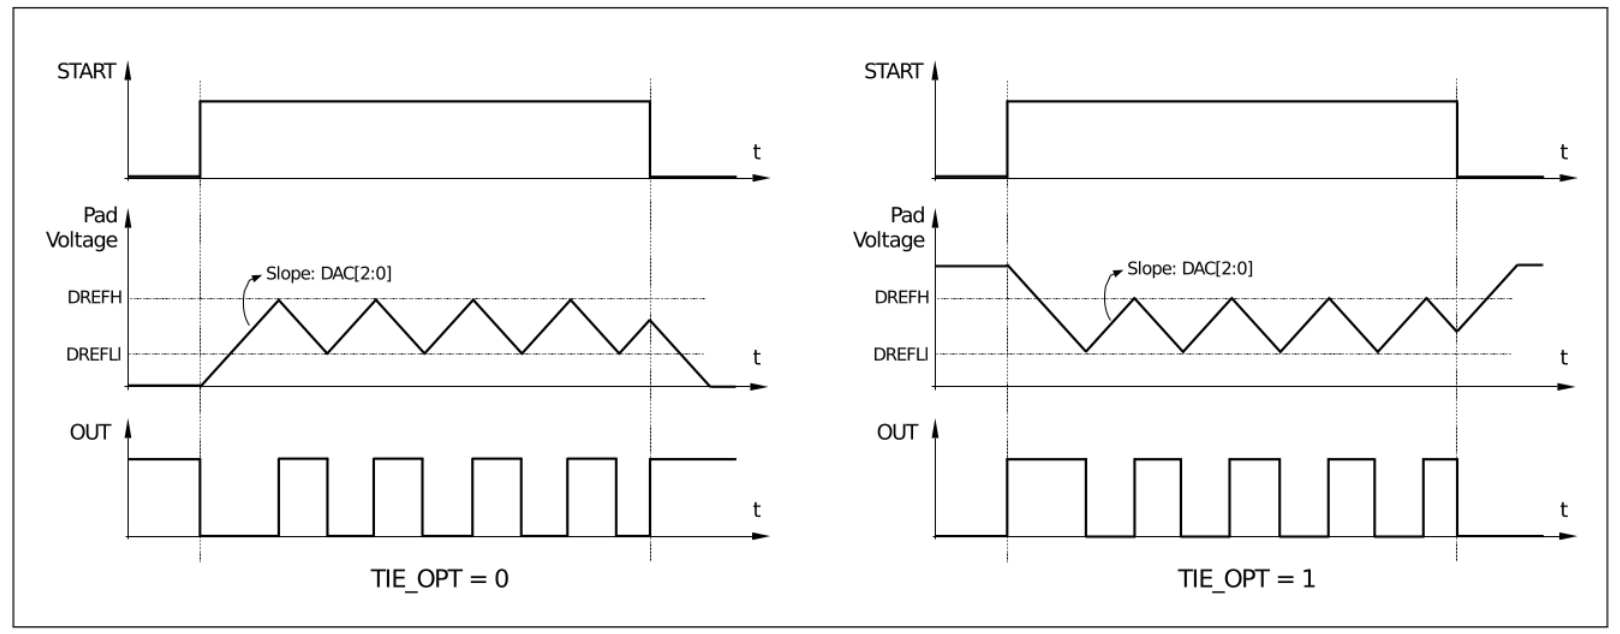
\includegraphics[width=12cm, height=6cm]{ESP32/Touch_Sensor_Operating_Flow.png}
		\caption{Touch Sensor Operating Flow} 
		\label{fig:Python 3.10.}
	\end{center}
\end{figure}	

\subsection{Installation}
Connecting the sound sensor to the microcontroller is simple, we just need to power the module with 3.3V power and connect the analog out pin to the ESP32. Now we can process the signal with the ADC of the ESP32. We have also connected three LEDs to show the intensity of the device and we are also showing the recorded decibel on the OLED display. The LEDs are connected to the GPIO pins of the ESP32 and the OLED module is connected to the I2C pins of the ESP32 device. Learn more about interfacing OLED with ESP32 here.
\\

Components Needed

\begin{enumerate}
	\item ESP32 Development Board
	\item Sound Sensor (e.g., KY-038, LM393)
	\item Connecting Wires
	\item Breadboard 
	\item Power Source  
\end{enumerate}

Step-by-Step Installation Guide
\begin{enumerate}
	\item VCC to 3V3: Connect the VCC pin of the sound sensor to the 3.3V pin on the ESP32.
	\item GND to GND: Connect the GND pin of the sound sensor to the GND pin on the ESP32.
	\item AO to GPIO34: Connect the Analog Output (AO) of the sound sensor to GPIO34 (or any other ADC pin) on the ESP32.
	\item DO to GPIO35: Connect the Digital Output (DO) of the sound sensor to GPIO35 (optional, only if you need digital signal).
\end{enumerate}


The following picture shows the KY-038 and also the KY-037 microphone module with all electronic parts.

\begin{figure}  
	\begin{center}
 		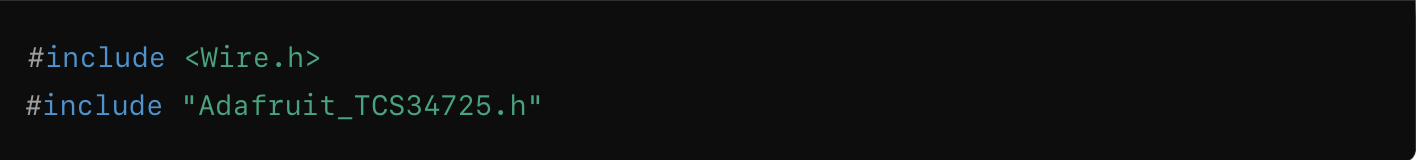
\includegraphics[width=12cm, height=6cm]{ESP32/color_sensor_1.png}
		\caption{Installation Sound Sensor} 
		\label{fig:Python 3.10.}
	\end{center}
\end{figure}	



\begin{figure}  
	\begin{center}
		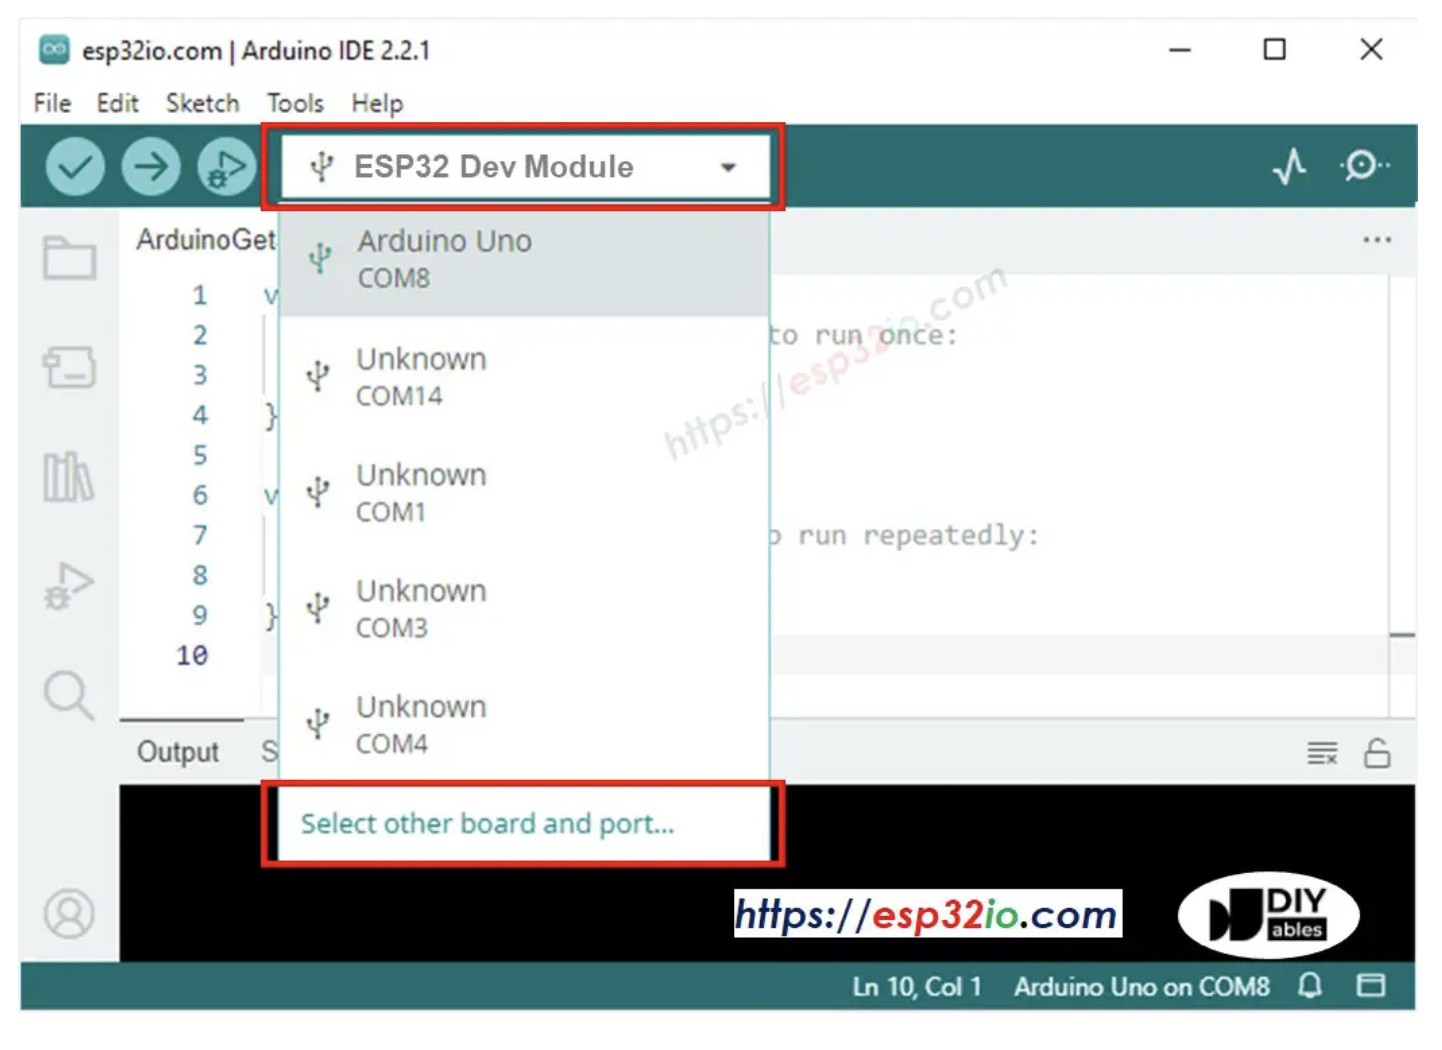
\includegraphics[width=12cm, height=6cm]{ESP32/installation_Touch_Sensor_2.png}
		\caption{Selection of esp32 board} 
		\label{fig:Python 3.10.}
	\end{center}
\end{figure}	

\subsection{Functions}
The basic functionality of the microphone is the same for the KY-038 and the KY-037. The microphone generates the input for the sound sensor module and consists of a thin diaphragm that is one plate of a capacitor. The second plate of the capacitor is the back plate and in parallel to the diaphragm in very close distance. The following picture shows a basic schematic of the microphone.

If someone speaks into the microphone, the sound waves created by the voice hit the diaphragm. Due to those hits, the diaphragm vibrates and therefore the distance between the two plates of the capacitor gets shorter or wider (picture on the left side).

Because the capacitance is directly proportional to the distance between the plates, the sound waves of the voice changes the voltage across the plates that has a direct influence of the circuit of the KY-038 and KY-037 sound sensor module.

\begin{figure}  
	\begin{center}
		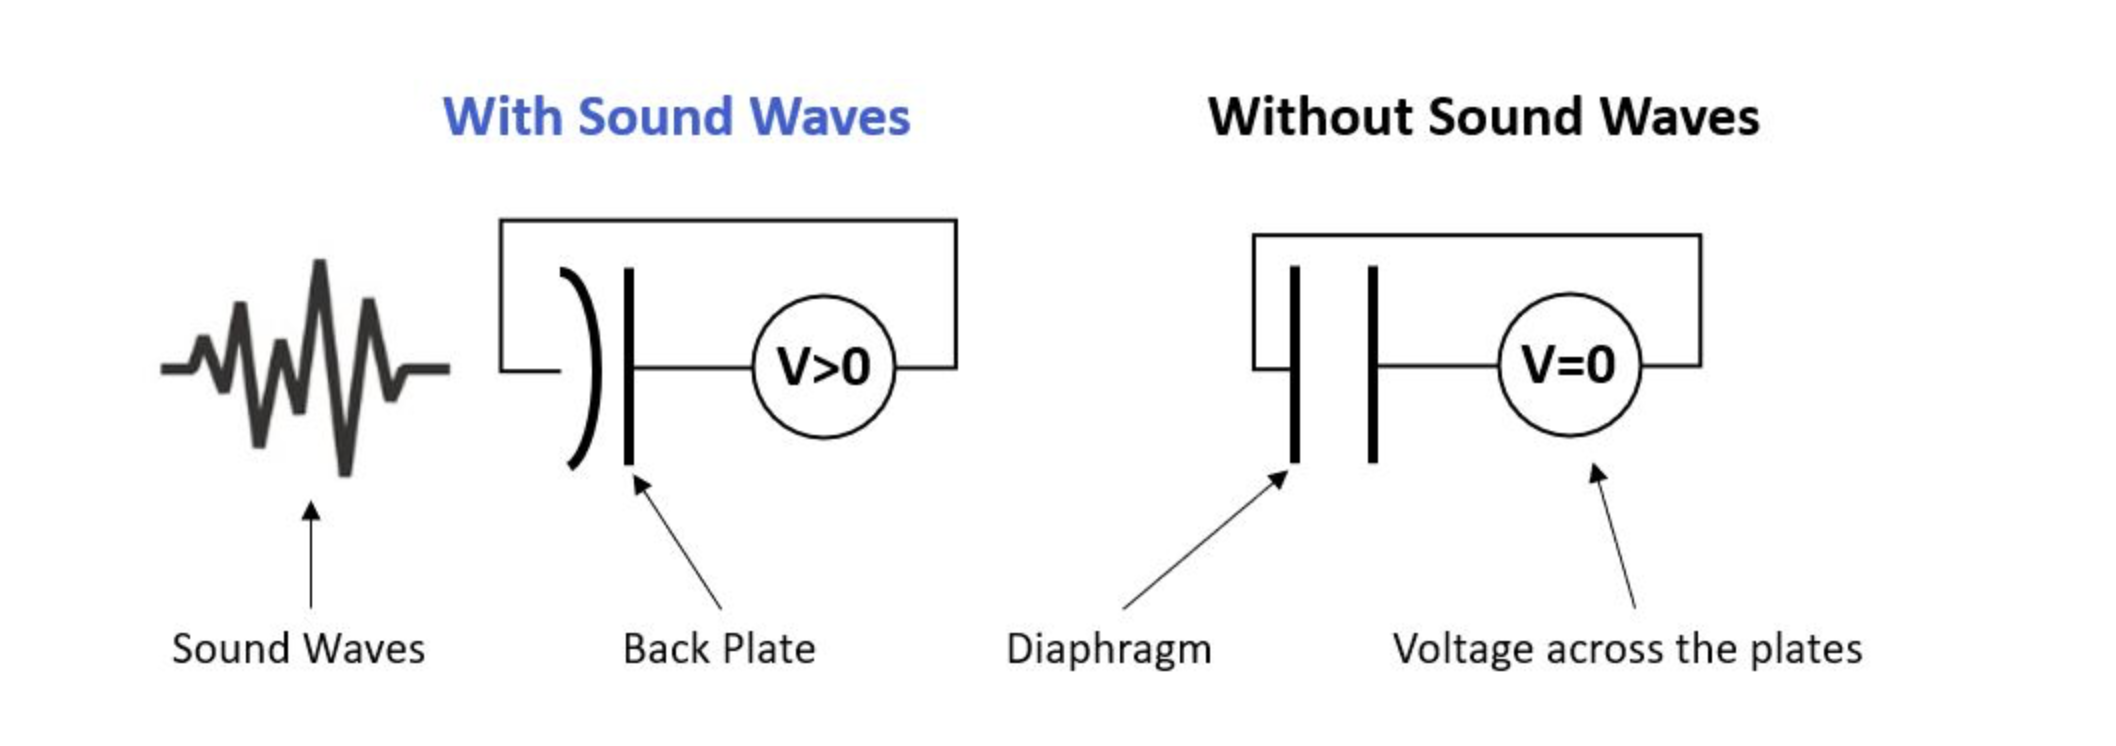
\includegraphics[width=12cm, height=6cm]{ESP32/sound_sensor_funcationality.png}
		\caption{Sound Sensor Funcationality} 
		\label{fig:Python 3.10.}
	\end{center}
\end{figure}	


\subsection{Example - Manual}

This example creates a capacitive touch slider using multiple touch pins to detect the position of the touch.


\begin{Arduino}

	
	#define SENSOR_PIN 18 // ESP32 pin GPIO18 connected to the OUT pin of the sound sensor
	
	int lastState = HIGH;  // the previous state from the input pin
	int currentState;      // the current reading from the input pin
	
	void setup() {
		// initialize serial communication at 9600 bits per second:
		Serial.begin(9600);
		// initialize the ESP32's pin as an input
		pinMode(SENSOR_PIN, INPUT);
	}
	
	void loop() {
		// read the state of the the ESP32's input pin
		currentState = digitalRead(SENSOR_PIN);
		
		if (lastState == HIGH && currentState == LOW)
		Serial.println("The sound has been detected");
		else if (lastState == LOW && currentState == HIGH)
		Serial.println("The sound has disappeared");
		
		// save the the last state
		lastState = currentState;
	}
	
	
	
	
\end{Arduino}


\begin{figure}  
	\begin{center}
		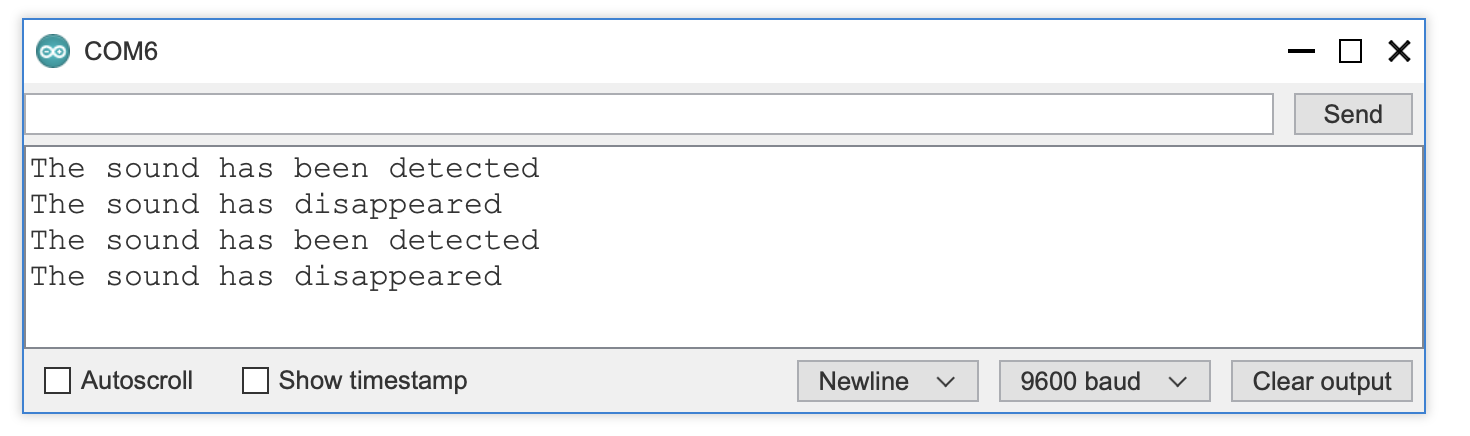
\includegraphics[width=12cm, height=6cm]{ESP32/sound_sensor_example.png}
		\caption{Sound Sensor Example} 
		\label{fig:Python 3.10.}
	\end{center}
\end{figure}	


Please keep in mind that if you notice the LED status remaining constantly on or off, even when there is sound present, you may need to adjust the potentiometer to fine-tune the sound sensitivity of the sensor.
Now, we have the freedom to personalize the code and make it trigger an LED or a light when sound is detected. We can even make a servo motor rotate according to the sound input. For more detailed guidance and step-by-step instructions, you can refer to the tutorials provided at the end of this tutorial.


\subsection{Example - Code}

\begin{Arduino}
	#include <Wire.h>
	
	#include <Adafruit_GFX.h>
	
	#include <Adafruit_SSD1306.h>
	
	#define  SCREEN_WIDTH 128 // OLED display width, in pixels
	
	#define  SCREEN_HEIGHT 64 // OLED display height, in pixels
	
	#define  OLED_RESET   -1 // Reset pin # (or -1 if sharing Arduino reset pin)
	
	
	
	Adafruit_SSD1306 display(SCREEN_WIDTH, SCREEN_HEIGHT, &Wire, OLED_RESET);
	
	
	
	const int sampleWindow = 50;
	
	unsigned int sample;
	
	
	
	#define SENSOR_PIN 35
	
	#define PIN_QUIET 33
	
	#define PIN_MODERATE 25
	
	#define PIN_LOUD 26
	
	
	
	void setup(){
		
		pinMode(SENSOR_PIN, INPUT); 
		
		pinMode(PIN_QUIET, OUTPUT);
		
		pinMode(PIN_MODERATE, OUTPUT);
		
		pinMode(PIN_LOUD, OUTPUT);
		
		
		
		digitalWrite(PIN_QUIET, LOW);
		
		digitalWrite(PIN_MODERATE, LOW);
		
		digitalWrite(PIN_LOUD, LOW);
		
		
		
		Serial.begin(115200);
		
		
		
		if (!display.begin(SSD1306_SWITCHCAPVCC, 0x3C)) {
			
			Serial.println(F("SSD1306 allocation failed"));
			
			for (;;); 
			
		}
		
		
		
		display.clearDisplay();
		
		display.setTextSize(2);
		
		display.setTextColor(WHITE);
		
		display.display();
		
		digitalWrite(PIN_LOUD, LOW);
		
	}
	
	
	
	void loop()
	
	{
		
		unsigned long startMillis = millis();                  
		
		float peakToPeak = 0;                                  
		
		
		
		unsigned int signalMax = 0;                            
		
		unsigned int signalMin = 1024;                         
		
		
		
		// collect data for 50 mS
		
		while (millis() - startMillis < sampleWindow)
		
		{
			
			sample = analogRead(SENSOR_PIN);
			
			
			
			if (sample < 1024)                                  
			
			{
				
				if (sample > signalMax)
				
				{
					
					signalMax = sample;                          
					
				}
				
				else if (sample < signalMin)
				
				{
					
					signalMin = sample;                           
					
				}
				
			}
			
		}
		
		peakToPeak = signalMax - signalMin;                    
		
		int db = map(peakToPeak, 0, 900, 49, 90);         
		
		Serial.print("\t");
		
		Serial.println(db);
		
		display.setCursor(0, 0);
		
		display.print("Loudness: ");
		
		display.print(db);
		
		display.print("dB");
		
		digitalWrite(PIN_LOUD, LOW);
		
		if (db <= 55)
		
		{
			
			
			
			display.clearDisplay();
			
			display.setCursor(0, 1);
			
			display.print("Level:Quite");
			
			display.display();
			
			digitalWrite(PIN_QUIET, HIGH);
			
			digitalWrite(PIN_MODERATE, LOW);
			
			digitalWrite(PIN_LOUD, LOW);
			
			//  delay(3000);
			
		}
		
		else if (db > 60 && db < 85)
		
		{
			
			display.clearDisplay();
			
			display.setCursor(0, 1);
			
			display.print("Level:Moderate");
			
			display.display();
			
			digitalWrite(PIN_QUIET, LOW);
			
			digitalWrite(PIN_MODERATE, HIGH);
			
			digitalWrite(PIN_LOUD, LOW);
			
		}
		
		else if (db >= 85 && db <= 90)
		
		{
			
			display.clearDisplay();
			
			display.setCursor(0, 1);
			
			display.print("Level:High");
			
			display.display();
			
			digitalWrite(PIN_QUIET, LOW);
			
			digitalWrite(PIN_MODERATE, LOW);
			
			digitalWrite(PIN_LOUD, HIGH);
			
		}
		
		else
		
		{
			
			digitalWrite(PIN_QUIET, LOW);
			
			digitalWrite(PIN_MODERATE, LOW);
			
			digitalWrite(PIN_LOUD, LOW);
			
		}
		
		
		
		delay(200);
		
	}
	
	
\end{Arduino}



\subsection{Example - Files}



\subsection{Calibration}

Calibration involves comparing the BH1750's readings with a known reference light meter under controlled lighting conditions and adjusting the readings accordingly.

Here’s a step-by-step guide to calibrate the BH1750:
cite method

\subsection{Simple Code}
This example reads the analog value from the sound sensor and prints it to the Serial Monitor

\begin{Arduino}
	#define SOUND_SENSOR_PIN 34  // Analog pin
	
	void setup() {
		Serial.begin(115200);
		pinMode(SOUND_SENSOR_PIN, INPUT);
	}
	
	void loop() {
		int soundLevel = analogRead(SOUND_SENSOR_PIN);
		Serial.println(soundLevel);
		delay(100);
	}
	
	
\end{Arduino}

\subsection{Simple Application}
This example uses the digital output of the sound sensor to detect if the sound level exceeds a certain threshold.

\begin{Arduino}
	#define SOUND_SENSOR_PIN 35  // Digital pin
	
	void setup() {
		Serial.begin(115200);
		pinMode(SOUND_SENSOR_PIN, INPUT);
	}
	
	void loop() {
		int soundDetected = digitalRead(SOUND_SENSOR_PIN);
		if (soundDetected == HIGH) {
			Serial.println("Sound detected!");
		} else {
			Serial.println("No sound.");
		}
		delay(100);
	}
	
	
\end{Arduino}




\subsection{Tests}

\subsection{Simple Function Test}

The simplest test is the flashing of the \ac{led} at 2 Hz.

{
	\captionof{code}{Simple sketch to test the power LED}\label{Nano:PowerLEDTest}
	\ArduinoExternal{}{../../Code/Nano33BLESense/Test/TestLEDPower.ino}
}


\subsection{Test all Functions}

The brightness of the power LED can be controlled. This is demonstrated in the example sketch \ref{Nano:PowerLEDTestPWM}.

Using the pulse width modulation, the brightness is gradually increased to the maximum value and then gradually reduced to 0 again.




{
	\captionof{code}{Simple sketch to check the battery state using the power LED}\label{Nano:PowerLEDTestPWM}
	\ArduinoExternal{}{../../Code/Nano33BLESense/Test/TestLEDPowerBrightness.ino}
}

\subsection{Simple Application}


There are different situations where it might be useful to program the power LED of the Arduino Nano. For example, you could use it to:

\begin{itemize}
	\item Indicate the status of the board, such as whether it is connected to a power source, a computer, or a sensor.
	\item  Display the battery level of the board, by changing the brightness or color of the power \ac{led}.
	\item Create a visual alarm or notification, by making the power LED blink or flash in a certain pattern.
\end{itemize}

\bigskip

A simple application is to check the condition of the battery. The sktech \ref{Nano:PowerLEDTestBattery} demonstrates, if the voltage drops too low, the power LED flashes.

{
	\captionof{code}{Simple sketch to check the battery state using the power LED}\label{Nano:PowerLEDTestBattery}
	\ArduinoExternal{}{../../Code/Nano33BLESense/Test/TestLEDPowerBattery.ino}
}

\section{Soil Moisture Sensors}
\subsection{Soil Moisture Sensors}

Soil moisture is basically the content of water present in the soil. This can be measured using a soil moisture sensor which consists of two conducting probes that act as a probe. It can measure the moisture content in the soil based on the change in resistance between the two conducting plates \cite{Aquino:2021}.

Soil moisture sensors are crucial tools in agricultural and horticultural practices, designed to measure the water content in the soil. These sensors provide real-time data that help farmers, gardeners, and researchers optimize irrigation practices, ensuring plants receive the appropriate amount of water. The core component of most soil moisture sensors is a probe that is inserted into the soil, which measures the volumetric water content through various methods such as capacitance, resistivity, or time-domain reflectometry (TDR). Capacitance sensors, for example, determine moisture levels by measuring the dielectric permittivity of the soil \cite{Korlepara:2024}, which changes with water content. Resistive sensors, on the other hand, measure the electrical resistance between two electrodes, which decreases as the soil moisture increases. Advanced sensors might also use TDR to measure the time it takes for an electromagnetic pulse to travel through the soil \cite{Mohammad:2023}.

These sensors are typically connected to microcontrollers or data loggers, which collect and analyze the data, often displaying it through user-friendly interfaces or transmitting it wirelessly for remote monitoring. The information gathered can be used to automate irrigation systems, reducing water wastage and promoting sustainable agricultural practices. Additionally, soil moisture sensors are invaluable in research settings, providing precise and repeatable measurements for studies on plant physiology, soil health, and climate interactions. By leveraging the accurate data provided by soil moisture sensors, users can make informed decisions that enhance crop yields, conserve water resources, and contribute to the overall health of the ecosystem.



\subsection{Specification}
\subsection{Soil Moisture Sensors}

The soil moisture sensor is designed to accurately measure the volumetric water content in soil, providing reliable data for irrigation management, agricultural research, and environmental monitoring. The sensor features a capacitive measurement principle, ensuring high sensitivity and minimal soil disturbance. It operates within a voltage range of 3.3V to 5V, making it compatible with a wide variety of microcontrollers and development boards, including Arduino and Raspberry Pi \cite{Maheswaran:2024}. The sensor outputs an analog signal that can be easily read and interpreted by standard analog-to-digital converters.

Constructed with corrosion-resistant materials, the sensor is suitable for long-term deployment in outdoor environments, withstanding varying soil conditions and moisture levels. The robust design includes a protective coating to shield the electronic components from moisture and mechanical damage. The sensor's compact size (measuring approximately 60mm x 20mm) allows for easy insertion into the soil without significant disruption to the soil structure \cite{Deepthi:2024}.

The soil moisture sensor boasts a measurement accuracy of ±3 and a resolution of 0.1, providing precise readings essential for optimizing irrigation schedules and improving crop yields. The response time is less than 1 second, ensuring real-time monitoring and adjustments. The sensor operates efficiently within a temperature range of -40°C to 85°C, accommodating various climatic conditions\cite{Rama:2021}.

Installation is straightforward: simply insert the sensor probes into the soil at the desired depth and connect the power and signal wires to the corresponding microcontroller pins. For enhanced performance, the sensor should

\subsection*{Electrical Characteristics}
\begin{itemize}
	\item \textbf{Operating Voltage:} 3.3V to 5V DC
	\item \textbf{Output Signal:} Analog voltage signal
	\item \textbf{Current Consumption:} < 20 mA
	\item \textbf{Interface:} 3-pin (VCC, GND, and AOUT)
\end{itemize}

\subsection*{Sensor Performance}
\begin{itemize}
	\item \textbf{Measurement Range:} 0-100\% volumetric water content
	\item \textbf{Accuracy:} ±3\% (typical)
	\item \textbf{Response Time:} < 1 second
	\item \textbf{Temperature Compensation:} Not included (external compensation recommended for precise measurements)
\end{itemize}

\subsection*{Physical Characteristics}
\begin{itemize}
	\item \textbf{Dimensions:} Typically around 60mm x 20mm x 5mm (varies by model)
	\item \textbf{Weight:} Approximately 10 grams
	\item \textbf{Material:} FR4 PCB with copper traces
	\item \textbf{Probes:} Dual metal probes (corrosion-resistant)
\end{itemize}

\subsection*{Environmental Specifications}
\begin{itemize}
	\item \textbf{Operating Temperature:} -10°C to 60°C
	\item \textbf{Storage Temperature:} -20°C to 70°C
	\item \textbf{Humidity:} 0-100\% RH (non-condensing)
\end{itemize}

\subsection*{Calibration and Usage}
\begin{itemize}
	\item \textbf{Calibration:} Manual calibration recommended for optimal accuracy
	\item \textbf{Installation:} Insert probes into the soil at the desired depth and location
	\item \textbf{Maintenance:} Periodic cleaning of probes to prevent soil buildup and corrosion
\end{itemize}

\subsection*{Compatibility}
\begin{itemize}
	\item \textbf{Microcontroller Compatibility:} Compatible with popular microcontrollers like Arduino, Raspberry Pi, ESP8266, and ESP32
	\item \textbf{Software Libraries:} Available libraries for Arduino IDE and Python for easy integration
\end{itemize}

\subsection*{Applications}
\begin{itemize}
	\item \textbf{Agriculture:} Automated irrigation systems, soil moisture monitoring
	\item \textbf{Horticulture:} Greenhouse and garden monitoring
	\item \textbf{Environmental Monitoring:} Soil health and moisture content studies
	\item \textbf{DIY Projects:} Home gardening, plant watering systems
\end{itemize}

\subsection{Bibliothek}

The Soil Moisture Sensor library is an essential tool for interfacing with soil moisture sensors using the Arduino platform. This library facilitates the reading of analog values from soil moisture sensors, providing a simple and efficient way to monitor soil moisture levels in various agricultural and gardening applications. By converting the analog signal into a readable value, the library allows users to determine the moisture content of the soil with high precision. Installation is straightforward through the Arduino IDE Library Manager, ensuring that even beginners can easily integrate soil moisture sensors into their projects. Additionally, the library includes functions for calibrating the sensor to account for different soil types, enhancing the accuracy of moisture readings. Overall, the Soil Moisture Sensor library is a robust and user-friendly tool for anyone looking to implement soil moisture monitoring in their Arduino-based projects.


\subsection{Description}

The soil moisture sensor is a crucial tool for monitoring and maintaining optimal soil conditions in agricultural, gardening, and environmental applications. This sensor measures the water content in the soil, providing real-time data that can be used to ensure plants receive the appropriate amount of water. The sensor typically consists of two conductive probes that are inserted into the soil. These probes form a variable resistor whose resistance changes depending on the moisture level: higher moisture results in lower resistance, while dry soil increases resistance.

When paired with an ESP32 microcontroller, the functionality and potential of the soil moisture sensor are significantly enhanced. The ESP32 is a powerful and versatile microcontroller with built-in Wi-Fi and Bluetooth capabilities. To use the soil moisture sensor with the ESP32, the sensor's analog output is connected to one of the ESP32's analog-to-digital converter (ADC) pins. This allows the ESP32 to read the sensor's analog signal, which reflects the soil's moisture level.

The ESP32 can process the sensor data to trigger various actions based on predefined thresholds. For instance, when the soil moisture level drops below a certain point, the ESP32 can activate a water pump or irrigation system to water the plants. This ensures that plants are watered only when necessary, conserving water and promoting healthy plant growth. Additionally, the ESP32 can send the soil moisture data to a cloud service or a remote server via its Wi-Fi connection. This enables real-time monitoring and data logging, allowing users to track soil moisture levels over time and make informed decisions about irrigation.

Furthermore, the ESP32’s low power consumption and deep sleep capabilities make it ideal for battery-operated or solar-powered systems, enhancing the sensor’s deployment in remote or off-grid locations. The connectivity options of the ESP32 also facilitate integration with other smart devices and systems, enabling more complex automation and control schemes. For example, the ESP32 can be programmed to adjust watering schedules based on weather forecasts or integrate with home automation systems for comprehensive environmental control.

\begin{figure}  
	\begin{center}
		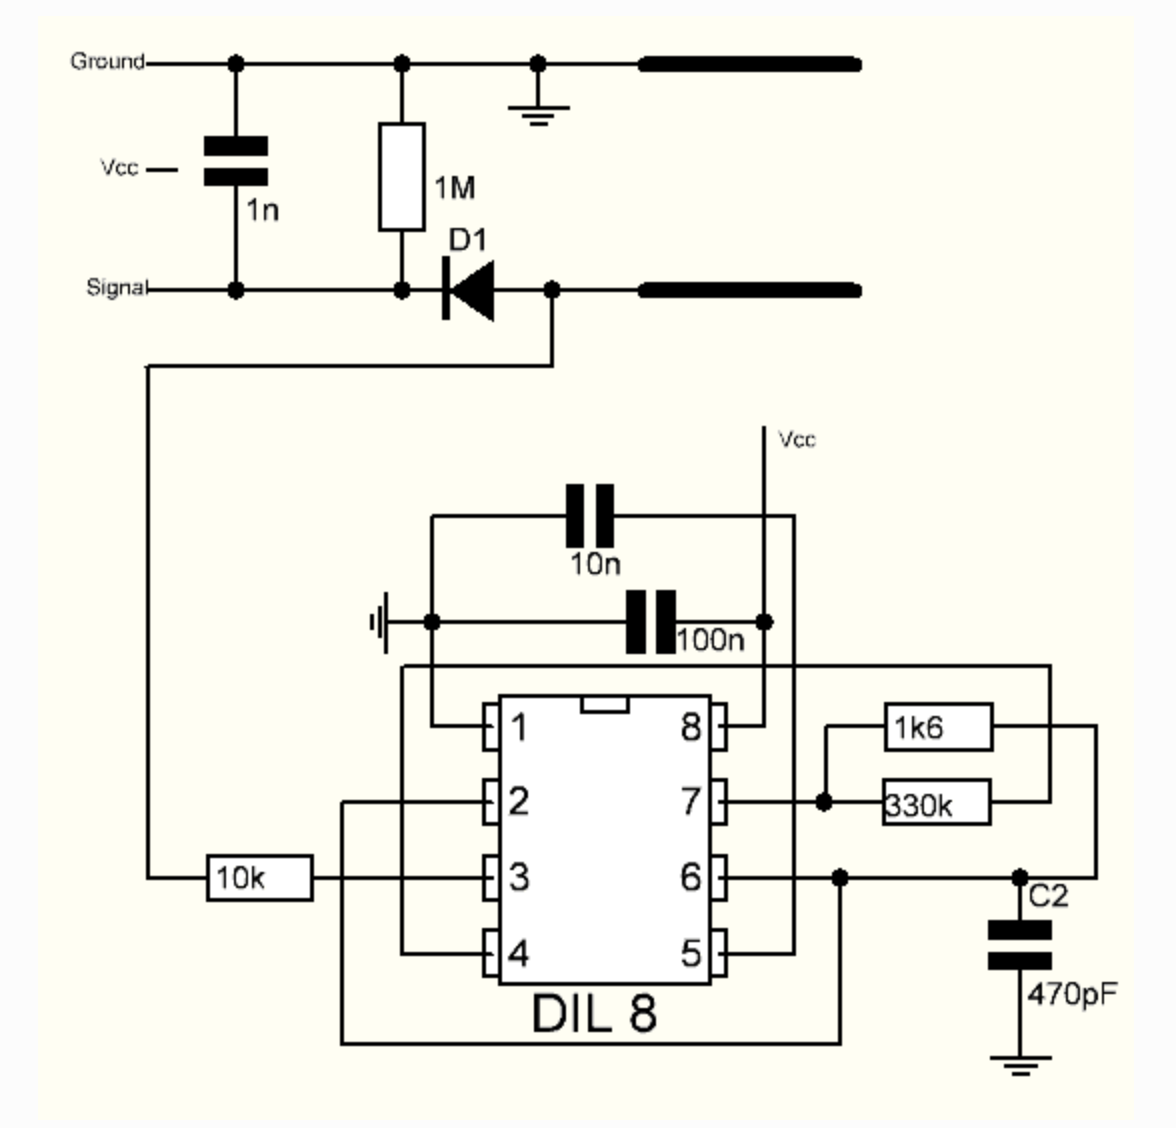
\includegraphics[width=12cm, height=6cm]{ESP32/Soil Moisture_1.png}
		\caption{Soil Sensor } 
		\label{fig:Python 3.10.}
	\end{center}
\end{figure}	

\subsection{Installation}
To install a color sensor on an ESP32, you will need to follow several steps to ensure proper wiring, library installation, and code implementation. Below is a comprehensive guide to help you through the process.

First, gather the necessary components: an ESP32 development board, a color sensor (such as the TCS34725), jumper wires, and a breadboard. Ensure that you have the latest version of the Arduino IDE installed on your computer, as this will be used to program the ESP32.

Begin by connecting the color sensor to the ESP32. The TCS34725 color sensor typically has four pins: VCC, GND, SDA, and SCL. Connect the VCC pin of the color sensor to the 3.3V pin on the ESP32 to provide power. Next, connect the GND pin of the sensor to a GND pin on the ESP32 to complete the circuit’s ground connection. The SDA (data line) pin of the color sensor should be connected to the ESP32’s GPIO21 pin, and the SCL (clock line) pin should be connected to the ESP32’s GPIO22 pin. If you are using a different color sensor, consult its datasheet for the appropriate connections.

Once the hardware is set up, proceed to install the necessary software libraries. Open the Arduino IDE and navigate to the Library Manager by selecting Sketch -> Include Library -> Manage Libraries. In the Library Manager, search for "Adafruit TCS34725" and install the library by Adafruit, which provides the necessary functions to interface with the TCS34725 sensor.

With the hardware connected and libraries installed, you can now write the code to interface with the color sensor. Start by including the necessary libraries in your Arduino sketch:

In the setup function, initialize the serial communication and check if the sensor is connected properly:

In the loop function, read the color values and print them to the Serial Monitor:
\\

With the hardware connected and libraries installed, you can now write the code to interface with the color sensor. Start by including the necessary libraries in your Arduino sketch:
\begin{figure}  
	\begin{center}
		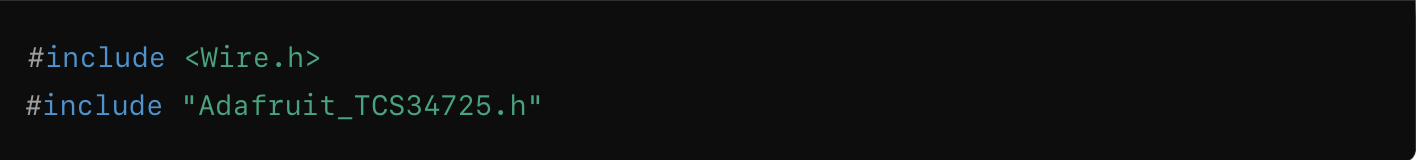
\includegraphics[width=12cm, height=2cm]{ESP32/color_sensor_1.png}
		\caption{Color Sensor  Instaltion} 
		\label{fig:Python 3.10.}
	\end{center}
\end{figure}	


In the setup function, initialize the serial communication and check if the sensor is connected properly:

\begin{figure}  
	\begin{center}
		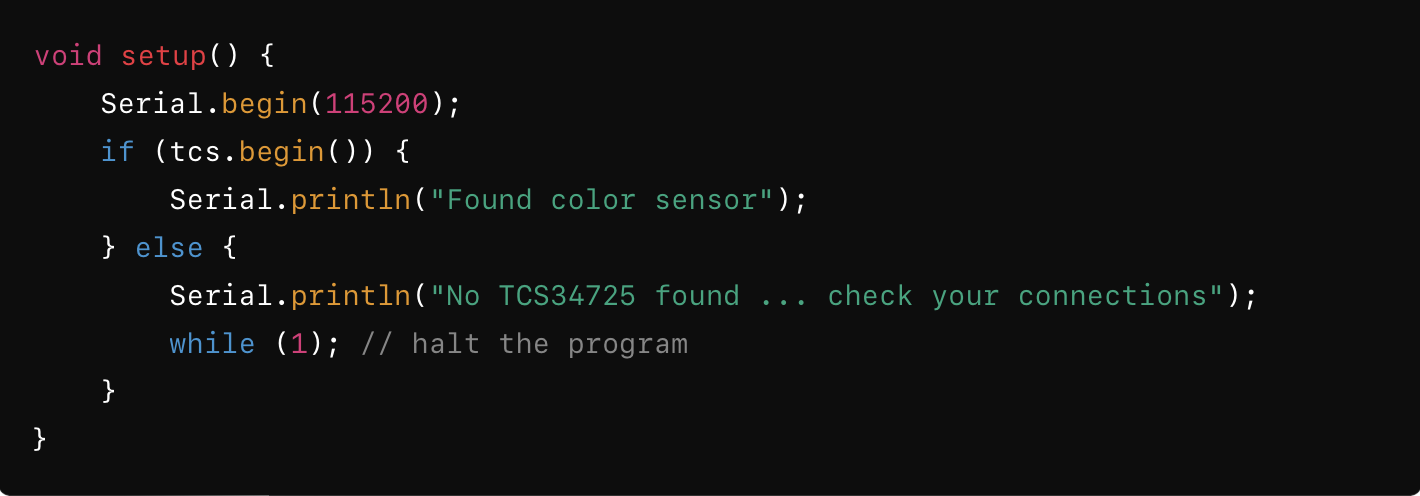
\includegraphics[width=12cm, height=6cm]{ESP32/color_sensor_2.png}
		\caption{Color Sensor Instaltion} 
		\label{fig:Python 3.10.}
	\end{center}
\end{figure}	

In the loop function, read the color values and print them to the Serial Monitor:
\begin{figure}  
	\begin{center}
		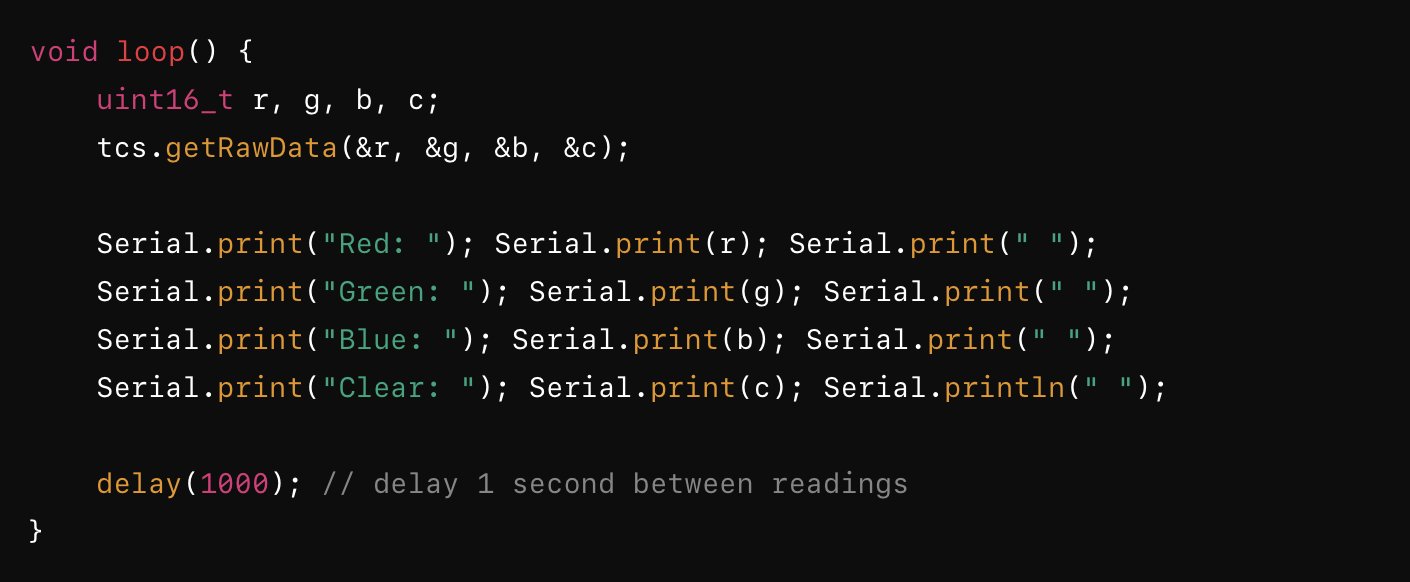
\includegraphics[width=12cm, height=6cm]{ESP32/color_sensor_3.png}
		\caption{Color Sensor Instaltion} 
		\label{fig:Python 3.10.}
	\end{center}
\end{figure}	



\subsection*{Requirements}



\subsubsection*{Hardware Requirements}

\begin{itemize}
	\item \textbf{ESP32 Development Board:} 
	\begin{itemize}
		\item A microcontroller with Wi-Fi and Bluetooth capabilities. Ensure the board has sufficient GPIO pins available for interfacing with the color sensor.
	\end{itemize}
	
	\item \textbf{Color Sensor Module:}
	\begin{itemize}
		\item A color sensor such as the TCS3200, TCS34725, or a similar module capable of detecting RGB values. The sensor should be compatible with 3.3V logic levels of the ESP32.
		\item The sensor must be capable of detecting the primary colors (Red, Green, Blue) and possibly other values such as Clear (C) for ambient light detection.
		\item Consider a sensor with an integrated IR filter to enhance accuracy by minimizing interference from infrared light.
	\end{itemize}
	
	\item \textbf{Pull-up Resistors (if required):}

	
	\item \textbf{Wiring and Connectors:}
	\begin{itemize}
		\item Jumper wires or a breadboard for initial prototyping.
		\item A secure connection method (such as soldering or using connectors) for final implementation to ensure stable and reliable sensor connections.
	\end{itemize}
	
	\item \textbf{Power Supply:}
	\begin{itemize}
		\item A stable 3.3V power source for both the ESP32 and the color sensor.
		\item Ensure the ESP32 can deliver sufficient current to power the sensor module, especially if other peripherals are connected.
	\end{itemize}
\end{itemize}

\subsubsection*{Software Requirements}

\begin{itemize}
	\item \textbf{ESP32 Arduino Core:}
	\begin{itemize}
		\item The ESP32 should be programmed using the Arduino IDE, so ensure the ESP32 board definitions are installed and up to date.
		\item Install the latest ESP32 core to ensure compatibility with libraries and functions required for sensor interfacing.
	\end{itemize}
	
	\item \textbf{Color Sensor Library:}
	\begin{itemize}
		\item Install the appropriate library for the specific color sensor being used (e.g., Adafruit TCS34725 library).
		\item The library should support I2C communication, which is common for color sensors like the TCS34725. Ensure the library is compatible with the ESP32.
		\item Example code or sketches should be available for quick testing and implementation.
	\end{itemize}
	
	\item \textbf{I2C Communication:}
	\begin{itemize}
		\item If using an I2C-based color sensor, ensure the ESP32 is configured correctly for I2C communication.
		\item The default I2C pins on the ESP32 are GPIO21 (SDA) and GPIO22 (SCL), but these can be changed in software if needed.
	\end{itemize}
	
	\item \textbf{Data Processing and Calibration:}
	\begin{itemize}
		\item Implement a calibration routine to account for variations in lighting conditions and sensor characteristics.
		\item The code should include functions to convert raw sensor readings (RGB values) into meaningful data, such as identifying specific colors or detecting changes in color.
	\end{itemize}
	
	\item \textbf{Power Management:}
	\begin{itemize}
		\item Include code to manage the power consumption of the ESP32 and the color sensor, especially in battery-powered applications.
		\item Utilize deep sleep modes on the ESP32 when the sensor is not actively needed to save power.
	\end{itemize}
	
	\item \textbf{Wi-Fi/Bluetooth Connectivity (Optional):}
	\begin{itemize}
		\item If wireless communication is required, implement Wi-Fi or Bluetooth functionality to transmit color data to a remote server or another device.
		\item Ensure that the additional processing and communication requirements do not interfere with the real-time operation of the color sensor.
	\end{itemize}
\end{itemize}

\subsubsection*{Environmental and Operational Requirements}

\begin{itemize}
	\item \textbf{Ambient Light Conditions:}
	\begin{itemize}
		\item The sensor should be capable of operating in varying ambient light conditions. If necessary, include a light shield or enclosure to minimize the effect of external light sources.
	\end{itemize}
	
	\item \textbf{Temperature and Humidity:}
	\begin{itemize}
		\item Ensure that both the ESP32 and the color sensor can operate within the expected temperature and humidity ranges of the application environment.
		\item Consider conformal coating or other protective measures if the sensor will be used in harsh environmental conditions.
	\end{itemize}
	
	\item \textbf{Mounting and Orientation:}
	\begin{itemize}
		\item Plan the physical placement of the color sensor carefully to ensure accurate color detection. The sensor should be positioned perpendicular to the surface being measured, with a consistent distance.
		\item Consider using a fixture or holder to maintain a stable position and orientation of the sensor.
	\end{itemize}
\end{itemize}

\subsection*{Circuit}

\subsubsection*{Components Required}
\begin{itemize}
	\item ESP32 Development Board
	\item TCS3200/TCS230 Color Sensor
	\item 10k ohm resistors (optional for pull-up)
	\item Breadboard and jumper wires
\end{itemize}

\subsubsection*{Circuit Connections}
\begin{itemize}
	\item \textbf{Power Supply:}
	\begin{itemize}
		\item Connect the \textbf{VCC} pin of the TCS3200 to the \textbf{3.3V} pin of the ESP32.
		\item Connect the \textbf{GND} pin of the TCS3200 to the \textbf{GND} pin of the ESP32.
	\end{itemize}
	\item \textbf{Control Pins (S0, S1, S2, S3):}
	\begin{itemize}
		\item Connect the \textbf{S0} pin to the \textbf{GPIO 25} of the ESP32.
		\item Connect the \textbf{S1} pin to the \textbf{GPIO 26} of the ESP32.
		\item Connect the \textbf{S2} pin to the \textbf{GPIO 27} of the ESP32.
		\item Connect the \textbf{S3} pin to the \textbf{GPIO 14} of the ESP32.
	\end{itemize}
	\item \textbf{Output Pin:}
	\begin{itemize}
		\item Connect the \textbf{OUT} pin of the TCS3200 to the \textbf{GPIO 34} of the ESP32.
	\end{itemize}
	\item \textbf{Output Enable (OE):}
	\begin{itemize}
		\item Connect the \textbf{OE} pin to \textbf{GND} to enable the output.
	\end{itemize}
	\item \textbf{Pull-up Resistor (Optional):}
	\begin{itemize}
		\item Place a 10k ohm pull-up resistor between the \textbf{S0} pin and \textbf{3.3V}.
	\end{itemize}
\end{itemize}


\subsection*{Installation Process}

installation process for a color sensor with an ESP32, formatted for LaTeX. This guide assumes you are using a common color sensor like the TCS3200 or TCS34725.


\subsection*{Materials Required}
\begin{itemize}
	\item ESP32 microcontroller board
	\item TCS34725 color sensor
	\item Breadboard and jumper wires
	\item 4.7k ohm pull-up resistors (optional, depending on sensor and wiring)
	\item Power source (e.g., USB power for the ESP32)
\end{itemize}

\subsection*{Wiring Diagram}
\begin{figure}[h]
	\centering
		\includegraphics[width=12cm, height=6cm]{ESP32/color_sensor_4.png}
	\caption{Wiring Diagram for TCS34725 Color Sensor with ESP32}
	\label{fig:wiring}
\end{figure}

\subsection*{Wiring Instructions}
Follow these steps to connect the TCS34725 color sensor to the ESP32:

\begin{enumerate}[label=\arabic*.]
	\item \textbf{Power Connection:}
	\begin{itemize}
		\item Connect the \textbf{VCC} pin of the TCS34725 sensor to the \textbf{3.3V} pin of the ESP32.
		\item Connect the \textbf{GND} pin of the TCS34725 sensor to the \textbf{GND} pin of the ESP32.
	\end{itemize}
	
	\item \textbf{I2C Communication:}
	\begin{itemize}
		\item Connect the \textbf{SCL} (Serial Clock) pin of the TCS34725 to the \textbf{GPIO 22} pin (SCL) of the ESP32.
		\item Connect the \textbf{SDA} (Serial Data) pin of the TCS34725 to the \textbf{GPIO 21} pin (SDA) of the ESP32.
	\end{itemize}
	
	\item \textbf{Pull-Up Resistors (Optional):}
	\begin{itemize}
		\item If necessary, place a 4.7k ohm pull-up resistor between the \textbf{VCC} and \textbf{SCL} pins.
		\item Similarly, place another 4.7k ohm pull-up resistor between the \textbf{VCC} and \textbf{SDA} pins. This helps to stabilize the I2C communication.
	\end{itemize}
	
	\item \textbf{Verify Connections:}
	\begin{itemize}
		\item Double-check all connections to ensure they are secure and correctly placed.
		\item Ensure the ESP32 and sensor are powered correctly.
	\end{itemize}
\end{enumerate}

\subsection*{Software Setup}

To interface with the TCS34725 sensor, you'll need to install the appropriate library and write a program to read color data. Follow these steps:

\begin{enumerate}[label=\arabic*.]
	\item \textbf{Install the Adafruit TCS34725 Library:}
	\begin{itemize}
		\item Open the Arduino IDE.
		\item Go to \textbf{Sketch} > \textbf{Include Library} > \textbf{Manage Libraries}.
		\item Search for \textbf{Adafruit TCS34725} and click \textbf{Install}.
	\end{itemize}
	
	\item \textbf{Upload Example Code:}
	\begin{itemize}
		\item Open the Arduino IDE and go to \textbf{File} > \textbf{Examples} > \textbf{Adafruit TCS34725} > \textbf{simpletest}.
		\item Connect the ESP32 to your computer and upload the code.
	\end{itemize}
	
	\item \textbf{Monitor Serial Output:}
	\begin{itemize}
		\item Open the Serial Monitor in the Arduino IDE (\textbf{Tools} > \textbf{Serial Monitor}).
		\item Set the baud rate to 9600.
		\item You should see the color readings being output to the Serial Monitor.
	\end{itemize}
\end{enumerate}

\subsection*{Troubleshooting Tips}
\begin{itemize}
	\item \textbf{No Output on Serial Monitor:}
	\begin{itemize}
		\item Verify that the sensor is correctly connected to the ESP32.
		\item Ensure that the I2C address used in the code matches the sensor’s address.
	\end{itemize}
	
	\item \textbf{Inconsistent or Erroneous Data:}
	\begin{itemize}
		\item Check the pull-up resistors on the I2C lines.
		\item Ensure that the sensor and ESP32 are properly powered.
	\end{itemize}
\end{itemize}


\subsection{Functions}
A soil moisture sensor measures the amount of water content in soil, which is crucial for monitoring plant health and optimizing irrigation. When used with an ESP32 microcontroller, the sensor can provide real-time data to help manage watering schedules and ensure plants receive the right amount of water \cite{Chhorn:2022}.

\subsection*{Soil Moisture Sensor Functions}

A soil moisture sensor is a device designed to measure the volumetric water \cite{Daniel:2021} content in soil. When used with an ESP32, it provides several key functions and benefits:

\begin{enumerate}[label=\arabic*.]
	\item \textbf{Soil Moisture Measurement}:
	\begin{itemize}
		\item The primary function of the sensor is to measure the amount of moisture present in the soil. It typically consists of two probes that detect the resistance of the soil, which varies with moisture content. The sensor converts this resistance into a voltage or digital signal that indicates soil moisture levels.
	\end{itemize}
	
	\item \textbf{Analog Signal Conversion}:
	\begin{itemize}
		\item Many soil moisture sensors output an analog voltage that is proportional to the soil moisture level. The ESP32 can read this analog signal using its built-in Analog-to-Digital Converter (ADC), which allows it to process and interpret the moisture levels.
	\end{itemize}
	
	\item \textbf{Digital Signal Output}:
	\begin{itemize}
		\item Some soil moisture sensors provide a digital output, often as a low or high signal depending on whether the moisture level is above or below a certain threshold. The ESP32 can read this digital signal to make simple decisions or trigger actions based on soil moisture.
	\end{itemize}
	
	\item \textbf{Integration with ESP32}:
	\begin{itemize}
		\item The ESP32 microcontroller can interface with the soil moisture sensor via its GPIO pins. For analog sensors, the ESP32 reads the voltage levels through its ADC. For digital sensors, it reads the signal as a binary state. The ESP32’s processing power and connectivity options (e.g., Wi-Fi and Bluetooth) allow it to use this data for various applications such as automated irrigation systems, data logging, or remote monitoring \cite{Didi:2022}.
	\end{itemize}
	
	\item \textbf{Data Processing and Communication}:
	\begin{itemize}
		\item The ESP32 can process the sensor data to determine the soil moisture level and make decisions based on this information. For example, it can control a relay to activate an irrigation system when soil moisture falls below a predefined threshold. Additionally, the ESP32 can send data to a remote server or display it on a web interface or mobile app, facilitating real-time monitoring and control.
	\end{itemize}
	
	\item \textbf{Calibration and Threshold Setting}:
	\begin{itemize}
		\item Calibration of the sensor may be necessary to ensure accurate readings. The ESP32 can be programmed to calibrate the sensor by comparing readings from the sensor under known moisture conditions. It can also be configured to set thresholds for moisture levels to automate actions or trigger alerts.
	\end{itemize}
\end{enumerate}

\begin{figure}  
	\begin{center}
		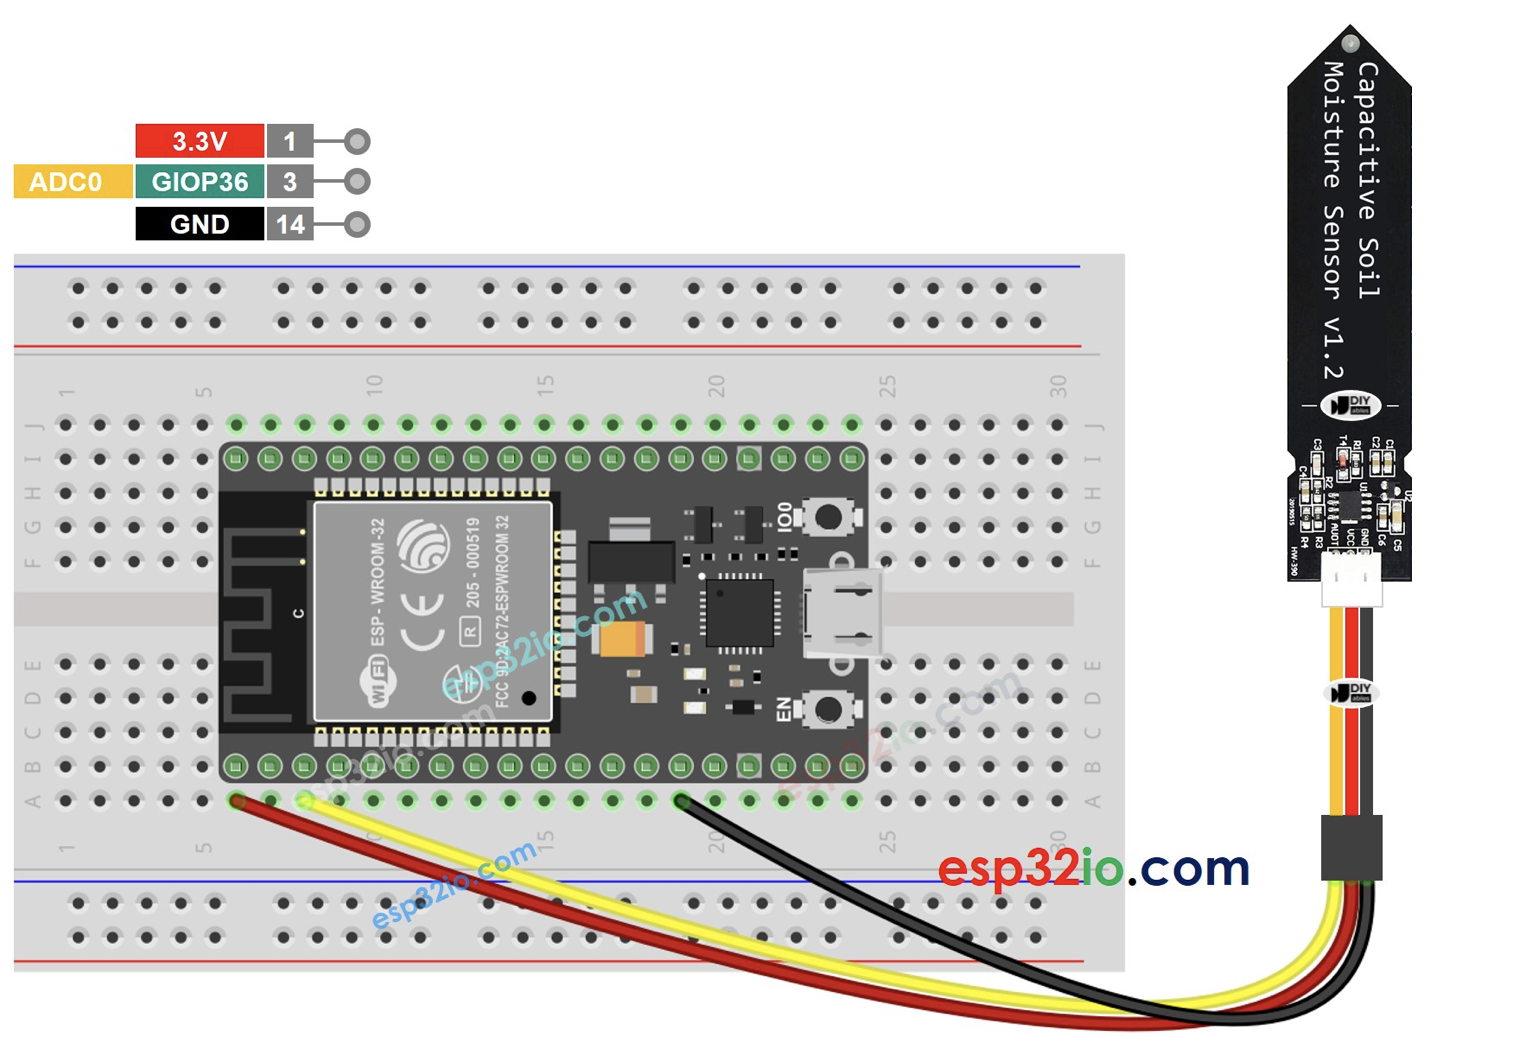
\includegraphics[width=12cm, height=6cm]{ESP32/Soil Moisture_3.png}
		\caption{Soil Sensor Funcationality} 
		\label{fig:Python 3.10.}
	\end{center}
\end{figure}	


\subsection{Example - Manual}

This example code demonstrates how to read soil moisture levels using a soil moisture sensor connected to an ESP32 microcontroller. The soil moisture sensor typically has an analog output that varies with the amount of moisture in the soil. This code reads the analog value from the sensor, converts it to a percentage, and prints it to the Serial Monitor.


\begin{Arduino}
	
	
	#include <Arduino.h>
	
	// Define the pin where the soil moisture sensor is connected
	const int moisturePin = 34; // Example pin; change according to your setup
	
	void setup() {
		// Start serial communication at 115200 baud rate
		Serial.begin(115200);
		
		// Initialize the analog pin
		pinMode(moisturePin, INPUT);
	}
	
	void loop() {
		// Read the analog value from the soil moisture sensor
		int sensorValue = analogRead(moisturePin);
		
		// Convert the analog value to a percentage (0-100%)
		// Assume sensor reads 0 when the soil is fully dry and 4095 when fully wet
		float percentage = map(sensorValue, 0, 4095, 0, 100);
		
		// Print the soil moisture percentage to the Serial Monitor
		Serial.print("Soil Moisture: ");
		Serial.print(percentage);
		Serial.println("%");
		
		// Wait for 1 second before taking another reading
		delay(1000);
	}
	
\end{Arduino}


\begin{figure}  
	\begin{center}
		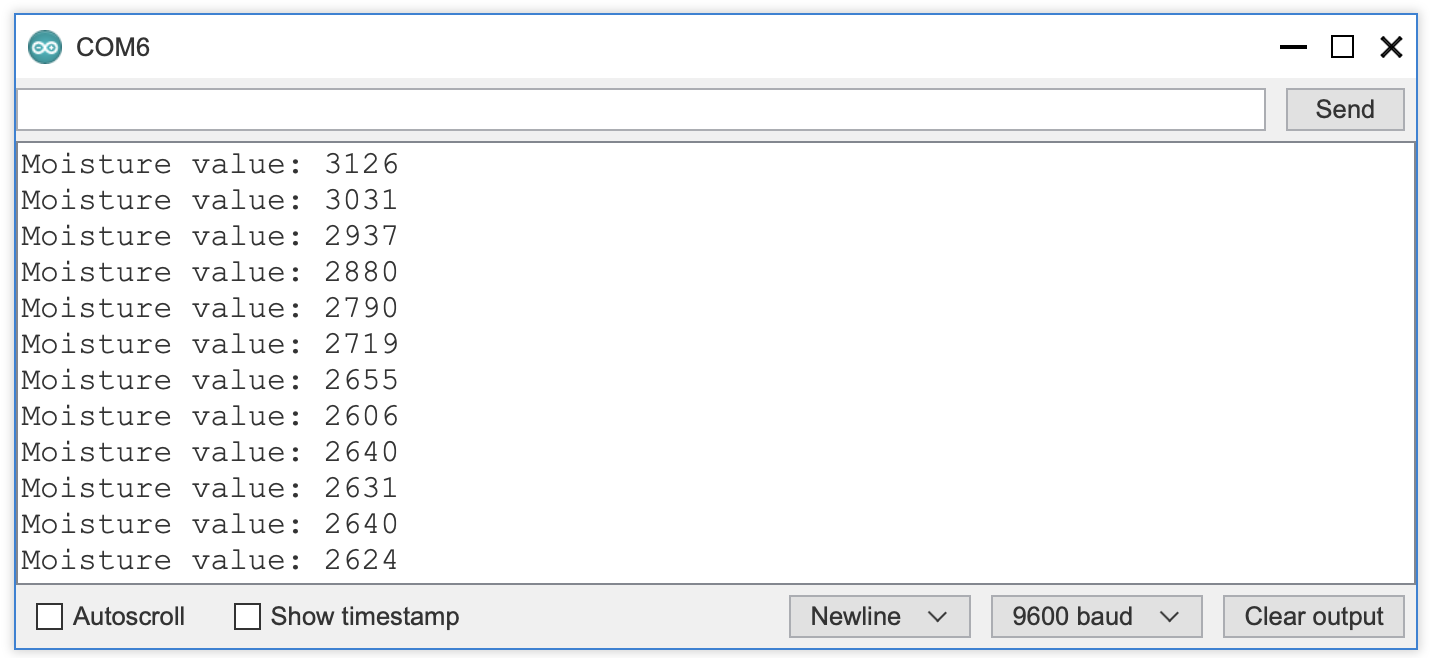
\includegraphics[width=12cm, height=6cm]{ESP32/Soil Moisture_4.png}
		\caption{Soil Sensor Example} 
		\label{fig:Python 3.10.}
	\end{center}
\end{figure}	



\subsection{Example - Code}
Reads raw analog values from the soil moisture sensor and prints them to the Serial Monitor.



\begin{Arduino}
	// Include the required libraries
	#include <WiFi.h>
	
	// Define the pin connected to the soil moisture sensor
	#define MOISTURE_SENSOR_PIN 34
	
	// Setup Wi-Fi credentials
	const char* ssid = "your_SSID";
	const char* password = "your_PASSWORD";
	
	// Variables to store the sensor reading and moisture threshold
	int moistureValue = 0;
	const int moistureThreshold = 500; // Change this value based on your calibration
	
	void setup() {
		// Initialize serial communication
		Serial.begin(115200);
		
		// Initialize the moisture sensor pin
		pinMode(MOISTURE_SENSOR_PIN, INPUT);
		
		// Connect to Wi-Fi
		WiFi.begin(ssid, password);
		Serial.print("Connecting to WiFi");
		while (WiFi.status() != WL_CONNECTED) {
			delay(500);
			Serial.print(".");
		}
		Serial.println("Connected!");
		Serial.print("IP Address: ");
		Serial.println(WiFi.localIP());
	}
	
	void loop() {
		// Read the moisture value from the sensor
		moistureValue = analogRead(MOISTURE_SENSOR_PIN);
		
		// Print the moisture value to the Serial Monitor
		Serial.print("Soil Moisture Value: ");
		Serial.println(moistureValue);
		
		// Check if the soil moisture is below the threshold
		if (moistureValue < moistureThreshold) {
			Serial.println("Soil is dry. Watering needed.");
		} else {
			Serial.println("Soil moisture is sufficient.");
		}
		
		// Wait before the next reading
		delay(2000); // Delay for 2 seconds
	}
	
	
	
\end{Arduino}



\subsection{Example - Files}



\subsection{Calibration}

Calibration involves comparing the BH1750's readings with a known reference light meter under controlled lighting conditions and adjusting the readings accordingly.

Here’s a step-by-step guide to calibrate the BH1750:
cite method

\subsection{Simple Code}
This example reads the analog value from the sound sensor and prints it to the Serial Monitor

\begin{Arduino}
	#define SOUND_SENSOR_PIN 34  // Analog pin
	
	void setup() {
		Serial.begin(115200);
		pinMode(SOUND_SENSOR_PIN, INPUT);
	}
	
	void loop() {
		int soundLevel = analogRead(SOUND_SENSOR_PIN);
		Serial.println(soundLevel);
		delay(100);
	}
	
	
\end{Arduino}

\subsection{Simple Application}
LED Control

\begin{Arduino}
	// Define the pins connected to the soil moisture sensor and LED
	#define MOISTURE_SENSOR_PIN 34
	#define LED_PIN 2
	
	// Define the moisture threshold
	const int moistureThreshold = 500; // Adjust based on calibration
	
	void setup() {
		// Initialize serial communication
		Serial.begin(115200);
		
		// Initialize the moisture sensor pin
		pinMode(MOISTURE_SENSOR_PIN, INPUT);
		
		// Initialize the LED pin
		pinMode(LED_PIN, OUTPUT);
		
		// Start with the LED turned off
		digitalWrite(LED_PIN, LOW);
	}
	
	void loop() {
		// Read the moisture value from the sensor
		int moistureValue = analogRead(MOISTURE_SENSOR_PIN);
		
		// Print the moisture value to the Serial Monitor
		Serial.print("Soil Moisture Value: ");
		Serial.println(moistureValue);
		
		// Control the LED based on soil moisture
		if (moistureValue < moistureThreshold) {
			// Soil is dry, turn on the LED
			digitalWrite(LED_PIN, HIGH);
			Serial.println("Soil is dry. LED ON.");
		} else {
			// Soil moisture is sufficient, turn off the LED
			digitalWrite(LED_PIN, LOW);
			Serial.println("Soil moisture is sufficient. LED OFF.");
		}
		
		// Wait before the next reading
		delay(2000); // Delay for 2 seconds
	}
	
	
	
\end{Arduino}




\subsection{Tests}

\subsection{Simple Function Test}

\begin{Arduino}
	// Define the pins connected to the soil moisture sensor and LED
	#define MOISTURE_SENSOR_PIN 34
	#define LED_PIN 2
	
	// Define the moisture threshold for testing
	const int moistureThreshold = 500; // Adjust based on calibration
	
	// Function prototypes
	void testSensor();
	void testLED();
	
	void setup() {
		// Initialize serial communication
		Serial.begin(115200);
		
		// Initialize the moisture sensor pin
		pinMode(MOISTURE_SENSOR_PIN, INPUT);
		
		// Initialize the LED pin
		pinMode(LED_PIN, OUTPUT);
		
		// Test the sensor and LED
		testSensor();
		testLED();
	}
	
	void loop() {
		// Continuously run the test functions
		testSensor();
		testLED();
		
		// Wait before repeating the test
		delay(5000); // Delay for 5 seconds
	}
	
	// Function to test the sensor
	void testSensor() {
		// Read the moisture value from the sensor
		int moistureValue = analogRead(MOISTURE_SENSOR_PIN);
		
		// Print the moisture value to the Serial Monitor
		Serial.print("Soil Moisture Value: ");
		Serial.println(moistureValue);
		
		// Check if the soil moisture is below the threshold
		if (moistureValue < moistureThreshold) {
			Serial.println("Soil is dry. Below threshold.");
		} else {
			Serial.println("Soil moisture is sufficient.");
		}
	}
	
	// Function to test the LED
	void testLED() {
		// Turn the LED on
		digitalWrite(LED_PIN, HIGH);
		Serial.println("LED ON");
		delay(1000); // Wait for 1 second
		
		// Turn the LED off
		digitalWrite(LED_PIN, LOW);
		Serial.println("LED OFF");
		delay(1000); // Wait for 1 second
	}
	
\end{Arduino}


\subsection{Test all Functions}

Below is a comprehensive test program for the ESP32 that includes functions to test the soil moisture sensor, LED control, and Wi-Fi connectivity. This program will help ensure that each component of your setup is working correctly.

\begin{Arduino}
	#include <WiFi.h>  // Include the Wi-Fi library for ESP32
	
	// Define the pins connected to the soil moisture sensor and LED
	#define MOISTURE_SENSOR_PIN 34
	#define LED_PIN 2
	
	// Define Wi-Fi credentials
	const char* ssid = "your_SSID";
	const char* password = "your_PASSWORD";
	
	// Define the moisture threshold for testing
	const int moistureThreshold = 500; // Adjust based on calibration
	
	// Function prototypes
	void testSensor();
	void testLED();
	void testWiFi();
	
	void setup() {
		// Initialize serial communication
		Serial.begin(115200);
		
		// Initialize the moisture sensor pin
		pinMode(MOISTURE_SENSOR_PIN, INPUT);
		
		// Initialize the LED pin
		pinMode(LED_PIN, OUTPUT);
		
		// Test the sensor, LED, and Wi-Fi
		testSensor();
		testLED();
		testWiFi();
	}
	
	void loop() {
		// Continuously run the test functions
		testSensor();
		testLED();
		testWiFi();
		
		// Wait before repeating the test
		delay(10000); // Delay for 10 seconds
	}
	
	// Function to test the soil moisture sensor
	void testSensor() {
		int moistureValue = analogRead(MOISTURE_SENSOR_PIN);
		
		Serial.print("Soil Moisture Value: ");
		Serial.println(moistureValue);
		
		if (moistureValue < moistureThreshold) {
			Serial.println("Soil is dry. Below threshold.");
		} else {
			Serial.println("Soil moisture is sufficient.");
		}
	}
	
	// Function to test the LED
	void testLED() {
		Serial.println("Testing LED...");
		
		// Turn the LED on
		digitalWrite(LED_PIN, HIGH);
		Serial.println("LED ON");
		delay(1000); // Wait for 1 second
		
		// Turn the LED off
		digitalWrite(LED_PIN, LOW);
		Serial.println("LED OFF");
		delay(1000); // Wait for 1 second
	}
	
	// Function to test Wi-Fi connectivity
	void testWiFi() {
		static bool connected = false;
		
		if (WiFi.status() != WL_CONNECTED) {
			Serial.print("Connecting to Wi-Fi");
			WiFi.begin(ssid, password);
			
			int attempts = 0;
			while (WiFi.status() != WL_CONNECTED && attempts < 30) {
				delay(500);
				Serial.print(".");
				attempts++;
			}
			
			if (WiFi.status() == WL_CONNECTED) {
				Serial.println("Connected!");
				Serial.print("IP Address: ");
				Serial.println(WiFi.localIP());
				connected = true;
			} else {
				Serial.println("Failed to connect.");
				connected = false;
			}
		} else if (!connected) {
			Serial.println("Already connected to Wi-Fi.");
			Serial.print("IP Address: ");
			Serial.println(WiFi.localIP());
			connected = true;
		}
	}
	
	
\end{Arduino}

\subsection{Simple Application}

Program for the ESP32 using a soil moisture sensor. This program reads the soil moisture level and controls an LED to indicate if the soil is too dry. If the soil moisture is below a certain threshold, the LED will turn on, signaling that watering is needed.

\begin{itemize}
	\item Indicate the status of the board, such as whether it is connected to a power source, a computer, or a sensor.
	\item  Display the battery level of the board, by changing the brightness or color of the power \ac{led}.
	\item Create a visual alarm or notification, by making the power LED blink or flash in a certain pattern.
\end{itemize}

\bigskip

A simple application is to check the condition of the battery. The sktech \ref{Nano:PowerLEDTestBattery} demonstrates, if the voltage drops too low, the power LED flashes.

{
	\captionof{code}{Simple sketch to check the battery state using the power LED}\label{Nano:PowerLEDTestBattery}
	\ArduinoExternal{}{../../Code/Nano33BLESense/Test/TestLEDPowerBattery.ino}
}

\section{Color Sensors Sensors}
\subsection{Color Sensors Sensors}

Color sensors are sophisticated electronic devices that are used to detect and measure colors in a variety of applications. They work by emitting light, typically from an LED, onto a target and then measuring the reflected light to determine the color composition. The primary components of a color sensor include a light source, a photodetector, and a filtering mechanism that segregates the reflected light into its primary color components – red, green, and blue (RGB). Advanced color sensors may also incorporate additional filters to enhance accuracy and may be capable of detecting a wider spectrum of colors.

The operating principle of color sensors is based on the fact that different colors reflect light differently. By analyzing the intensity of the reflected light across the RGB spectrum, the sensor can deduce the precise color of the object. This process typically involves converting the light intensity into electrical signals, which are then processed by a microcontroller or a similar processing unit to interpret the color data. Modern color sensors often come with integrated processing units that simplify the interface and provide digital outputs that are easy to integrate with various systems.

Color sensors find widespread use in numerous industries. In manufacturing, they are employed for quality control to ensure product colors are consistent and meet specified standards. In the automotive industry, they help in matching paint colors and in detecting color-coded wires during assembly. Consumer electronics, such as smartphones and cameras, utilize color sensors to adjust screen brightness and to enhance image quality. Additionally, color sensors play a crucial role in medical diagnostics, where they are used in devices to analyze biological samples based on color changes.

The versatility and precision of color sensors make them indispensable in applications that require accurate color detection and analysis. They are designed to operate under various lighting conditions and can be fine-tuned for specific applications, providing reliable performance across different environments. With advancements in technology, modern color sensors are becoming more compact, efficient, and capable of integrating with smart systems, paving the way for new and innovative applications in both existing and emerging fields.



\subsection{Specification}
\subsection{Color Sensors Sensors}

Color sensors are crucial components in many applications requiring color detection and differentiation. When interfacing with the ESP32, a versatile and powerful microcontroller, these sensors can provide precise and reliable color measurements. One popular color sensor is the TCS34725, which offers RGB and Clear light sensing with a digital output. The sensor operates on a voltage range of 3.0V to 3.6V, making it well-suited for direct interfacing with the ESP32's GPIO pins. The TCS34725 features an IR blocking filter and programmable gain and integration time, enhancing its accuracy and adaptability in various lighting conditions.

The sensor communicates with the ESP32 via the I2C protocol, utilizing the standard SDA and SCL lines. It has an I2C address of 0x29, which can be modified for multiple sensor applications. The integration of an LED on the sensor module assists in providing a consistent light source for accurate color measurements, particularly in environments with variable lighting. The TCS34725 boasts a high dynamic range of up to 3,800,000:1 and a maximum output frequency of 400 kHz in fast-mode plus, ensuring rapid and accurate color data transmission to the ESP32.

The TCS34725 includes a high sensitivity photodiode array capable of detecting a wide spectrum of colors. It provides 16-bit resolution output for each color channel (Red, Green, Blue, and Clear), enabling precise color detection and differentiation. The sensor also supports adjustable integration times ranging from 2.4 milliseconds to 700 milliseconds, allowing for fine-tuning based on specific application requirements and lighting conditions.

With its compact form factor, the TCS34725 can be easily integrated into various projects, such as color recognition in robotics, ambient light sensing, and industrial process control. The ESP32, with its dual-core processor, extensive GPIO options, and built-in Wi-Fi and Bluetooth capabilities, serves as an ideal companion for the TCS34725, facilitating complex data processing and wireless communication for IoT applications.

Overall, the combination of the TCS34725 color sensor and the ESP32 microcontroller provides a powerful and flexible solution for applications requiring accurate color detection and analysis. The ease of integration, robust communication protocol, and high precision of the TCS34725, coupled with the processing power and connectivity options of the ESP32, make this pairing suitable for a wide range of innovative projects.

Installation is straightforward: simply insert the sensor probes into the soil at the desired depth and connect the power and signal wires to the corresponding microcontroller pins. For enhanced performance, the sensor should

\subsection*{ Characteristics}
\begin{itemize}
	\item \textbf{Voltage Range:} Specifies the operating voltage range suitable for the ESP32.
	\item \textbf{Communication Protocol:} Describes the I2C protocol, including the standard lines and the I2C address.
	\item \textbf{Integrated LED:} Highlights the integrated LED for consistent lighting.
	\item \textbf{Dynamic Range and Frequency:}  Provides information on the sensor's dynamic range and output frequency.
   \item \textbf{Photodiode Array and Resolution:}  Details the sensor's capability to detect a wide spectrum of colors and its resolution.
   \item \textbf{Adjustable Integration Times:} Mentions the flexibility in adjusting integration times.
   \item \textbf{Form Factor and Applications:}  Discusses the compact size and potential applications.
   \item \textbf{ESP32 Features: } Explains why the ESP32 is an ideal companion for the color sensor.
\end{itemize}


\subsection{Bibliothek}

Color sensors are an essential component in various applications, such as robotics, automation, and color detection systems. One of the popular color sensors used in conjunction with the ESP32 microcontroller is the TCS3200/TCS34725. These sensors are capable of detecting the color of an object by measuring the intensity of light reflected from the object through different color filters. The ESP32, with its powerful processing capabilities and versatile connectivity options, provides an excellent platform for integrating and using these color sensors.

The TCS3200/TCS34725 color sensors contain an array of photodetectors, each with different filters for red, green, blue, and clear light. The sensor outputs a frequency that is directly proportional to the intensity of the detected color. The ESP32 can read these frequency outputs using its digital I/O pins and process the data to determine the color of the object. To facilitate the use of color sensors with the ESP32, the Adafruit TCS34725 library can be utilized. This library provides a user-friendly interface for configuring the sensor, reading color data, and converting the raw sensor readings into meaningful RGB values.

To set up the color sensor with the ESP32, connect the VCC and GND pins of the sensor to the 3.3V and GND pins of the ESP32, respectively. Connect the SDA and SCL pins of the sensor to the corresponding I2C pins on the ESP32 (usually GPIO21 for SDA and GPIO22 for SCL). The Adafruit TCS34725 library, which can be installed via the Arduino IDE Library Manager, simplifies the initialization and data retrieval process. Once the library is installed, the sensor can be initialized in the code using the `TCS34725 tcs = TCS34725(TCS34725INTEGRATIONTIME50MS, TCS34725GAIN1X);` command. The `tcs.getRawData(r, g, b, c);` function can then be used to read the raw color data.

In conclusion, the integration of TCS3200/TCS34725 color sensors with the ESP32 provides a robust solution for color detection and measurement tasks. The use of the Adafruit TCS34725 library significantly simplifies the development process, allowing for efficient and accurate color data acquisition. This combination is well-suited for a wide range of applications requiring precise color recognition and processing.




\subsection{Description}

When used in conjunction with an ESP32 microcontroller, color sensors offer enhanced capabilities due to the ESP32's robust processing power, wireless communication features, and versatile I/O interfaces. The ESP32 can process data from the color sensor and make real-time decisions or adjustments based on the detected colors. For example, in a robotics application, a color sensor connected to an ESP32 can be used to identify and sort objects based on their color, significantly enhancing the robot's ability to interact with its environment.

The integration process involves connecting the sensor to the ESP32's I/O pins. Typically, the sensor will have a few main connections: VCC for power, GND for ground, and several data lines (usually SDA and SCL for I2C communication, or a single data line for simpler sensors). The ESP32, equipped with built-in I2C hardware, can communicate with the sensor efficiently, retrieving the RGB values. Libraries such as the Adafruit TCS34725 library, designed for the popular TCS34725 color sensor, simplify this process by providing ready-to-use functions for sensor initialization, reading color values, and converting these values to more user-friendly formats like hexadecimal color codes.

Moreover, the ESP32's Wi-Fi and Bluetooth capabilities enable remote monitoring and control of the color sensor system. This is particularly useful in applications like smart homes, where color sensors can be used to adjust lighting conditions automatically based on the time of day or user preferences. The ESP32 can send the color data to a cloud server or a mobile app, allowing users to monitor the color measurements and configure the system remotely.

In conclusion, color sensors, when paired with the versatile ESP32 microcontroller, offer powerful and flexible solutions for a wide range of applications. The ESP32 enhances the sensor's functionality with its advanced processing, communication capabilities, and ease of integration, making it an ideal choice for projects requiring precise color detection and smart decision-making based on color data.

\begin{figure}  
	\begin{center}
		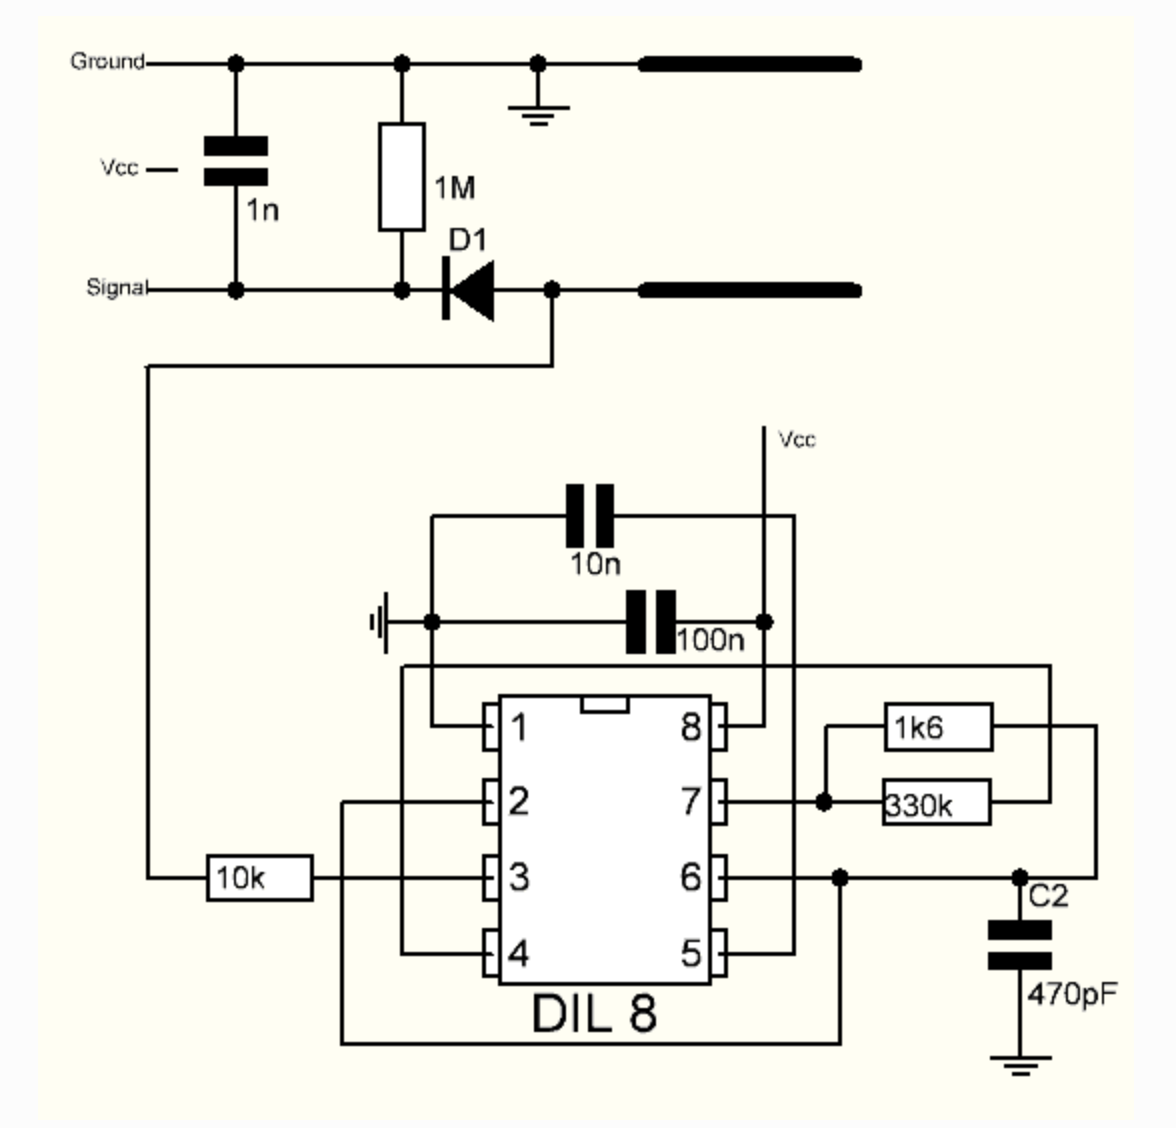
\includegraphics[width=12cm, height=6cm]{ESP32/Soil Moisture_1.png}
		\caption{Soil Sensor } 
		\label{fig:Python 3.10.}
	\end{center}
\end{figure}	

\subsection{Installation}
To install a color sensor on an ESP32, you will need to follow several steps to ensure proper wiring, library installation, and code implementation. Below is a comprehensive guide to help you through the process.

First, gather the necessary components: an ESP32 development board, a color sensor (such as the TCS34725), jumper wires, and a breadboard. Ensure that you have the latest version of the Arduino IDE installed on your computer, as this will be used to program the ESP32.

Begin by connecting the color sensor to the ESP32. The TCS34725 color sensor typically has four pins: VCC, GND, SDA, and SCL. Connect the VCC pin of the color sensor to the 3.3V pin on the ESP32 to provide power. Next, connect the GND pin of the sensor to a GND pin on the ESP32 to complete the circuit's ground connection. The SDA (data line) pin of the color sensor should be connected to the ESP32’s GPIO21 pin, and the SCL (clock line) pin should be connected to the ESP32’s GPIO22 pin. If you are using a different color sensor, consult its datasheet for the appropriate connections.

Once the hardware is set up, proceed to install the necessary software libraries. Open the Arduino IDE and navigate to the Library Manager by selecting Sketch -> Include Library -> Manage Libraries. In the Library Manager, search for "Adafruit TCS34725" and install the library by Adafruit, which provides the necessary functions to interface with the TCS34725 sensor.
\\

With the hardware connected and libraries installed, you can now write the code to interface with the color sensor. Start by including the necessary libraries in your Arduino sketch:
\begin{figure}  
	\begin{center}
		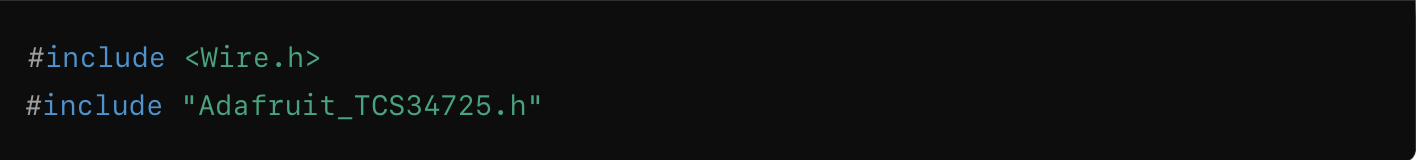
\includegraphics[width=12cm, height=6cm]{ESP32/color_sensor_1.png}
		\caption{Color Sensor Instalation} 
		\label{fig:Python 3.10.}
	\end{center}
\end{figure}	

In the setup function, initialize the serial communication and check if the sensor is connected properly:


\begin{figure}  
	\begin{center}
		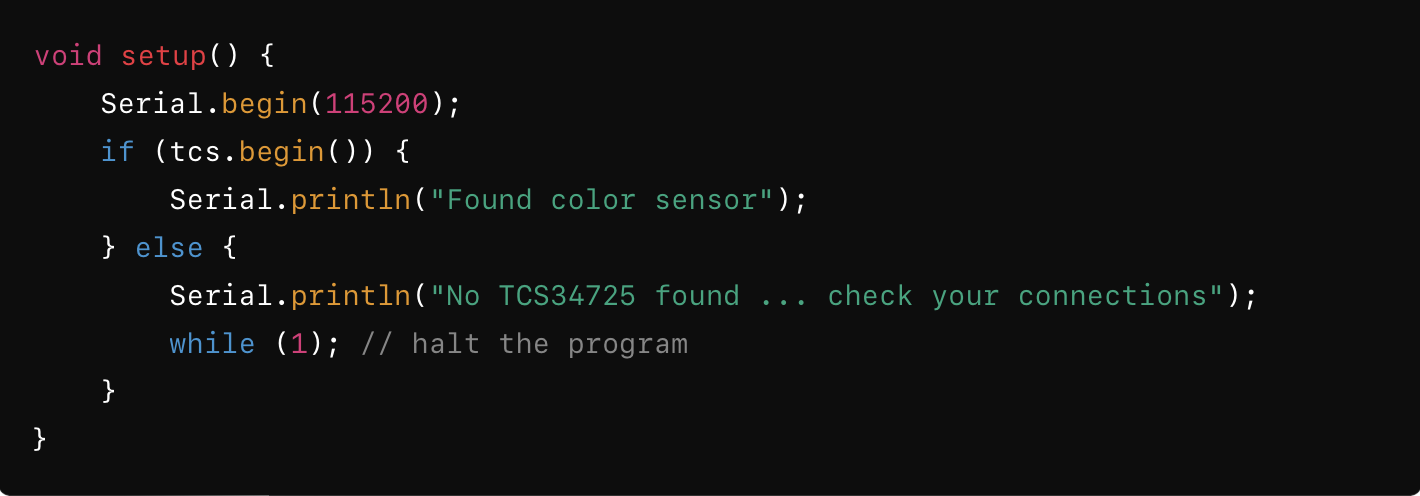
\includegraphics[width=12cm, height=6cm]{ESP32/color_sensor_2.png}
		\caption{Color Sensor Instalation} 
		\label{fig:Python 3.10.}
	\end{center}
\end{figure}	

In the loop function, read the color values and print them to the Serial Monitor:

\begin{figure}  
	\begin{center}
		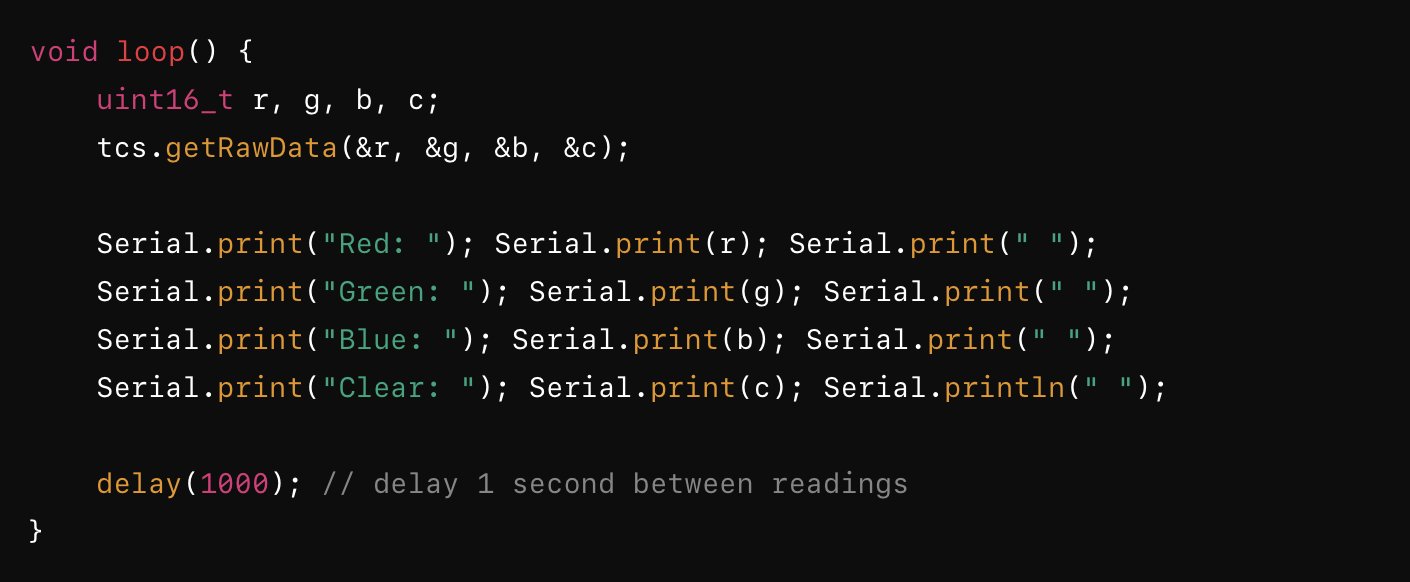
\includegraphics[width=12cm, height=6cm]{ESP32/color_sensor_3.png}
		\caption{Color Sensor Instalation} 
		\label{fig:Python 3.10.}
	\end{center}
\end{figure}	

\subsection*{Requirements}

\subsubsection*{Hardware Requirements}

\begin{itemize}
	\item \textbf{ESP32 Development Board:} 
	\begin{itemize}
		\item A microcontroller with Wi-Fi and Bluetooth capabilities. Ensure the board has sufficient GPIO pins available for interfacing with the color sensor.
	\end{itemize}
	
	\item \textbf{Color Sensor Module:}
	\begin{itemize}
		\item A color sensor such as the TCS3200, TCS34725, or a similar module capable of detecting RGB values. The sensor should be compatible with 3.3V logic levels of the ESP32.
		\item The sensor must be capable of detecting the primary colors (Red, Green, Blue) and possibly other values such as Clear (C) for ambient light detection.
		\item Consider a sensor with an integrated IR filter to enhance accuracy by minimizing interference from infrared light.
	\end{itemize}
	
	\item \textbf{Pull-up Resistors (if required):}

	
	\item \textbf{Wiring and Connectors:}
	\begin{itemize}
		\item Jumper wires or a breadboard for initial prototyping.
		\item A secure connection method (such as soldering or using connectors) for final implementation to ensure stable and reliable sensor connections.
	\end{itemize}
	
	\item \textbf{Power Supply:}
	\begin{itemize}
		\item A stable 3.3V power source for both the ESP32 and the color sensor.
		\item Ensure the ESP32 can deliver sufficient current to power the sensor module, especially if other peripherals are connected.
	\end{itemize}
\end{itemize}

\subsubsection*{Software Requirements}

\begin{itemize}
	\item \textbf{ESP32 Arduino Core:}
	\begin{itemize}
		\item The ESP32 should be programmed using the Arduino IDE, so ensure the ESP32 board definitions are installed and up to date.
		\item Install the latest ESP32 core to ensure compatibility with libraries and functions required for sensor interfacing.
	\end{itemize}
	
	\item \textbf{Color Sensor Library:}
	\begin{itemize}
		\item Install the appropriate library for the specific color sensor being used (e.g., Adafruit TCS34725 library).
		\item The library should support I2C communication, which is common for color sensors like the TCS34725. Ensure the library is compatible with the ESP32.
		\item Example code or sketches should be available for quick testing and implementation.
	\end{itemize}
	
	\item \textbf{I2C Communication:}
	\begin{itemize}
		\item If using an I2C-based color sensor, ensure the ESP32 is configured correctly for I2C communication.
		\item The default I2C pins on the ESP32 are GPIO21 (SDA) and GPIO22 (SCL), but these can be changed in software if needed.
	\end{itemize}
	
	\item \textbf{Data Processing and Calibration:}
	\begin{itemize}
		\item Implement a calibration routine to account for variations in lighting conditions and sensor characteristics.
		\item The code should include functions to convert raw sensor readings (RGB values) into meaningful data, such as identifying specific colors or detecting changes in color.
	\end{itemize}
	
	\item \textbf{Power Management:}
	\begin{itemize}
		\item Include code to manage the power consumption of the ESP32 and the color sensor, especially in battery-powered applications.
		\item Utilize deep sleep modes on the ESP32 when the sensor is not actively needed to save power.
	\end{itemize}
	
	\item \textbf{Wi-Fi/Bluetooth Connectivity (Optional):}
	\begin{itemize}
		\item If wireless communication is required, implement Wi-Fi or Bluetooth functionality to transmit color data to a remote server or another device.
		\item Ensure that the additional processing and communication requirements do not interfere with the real-time operation of the color sensor.
	\end{itemize}
\end{itemize}

\subsubsection*{Environmental and Operational Requirements}

\begin{itemize}
	\item \textbf{Ambient Light Conditions:}
	\begin{itemize}
		\item The sensor should be capable of operating in varying ambient light conditions. If necessary, include a light shield or enclosure to minimize the effect of external light sources.
	\end{itemize}
	
	\item \textbf{Temperature and Humidity:}
	\begin{itemize}
		\item Ensure that both the ESP32 and the color sensor can operate within the expected temperature and humidity ranges of the application environment.
		\item Consider conformal coating or other protective measures if the sensor will be used in harsh environmental conditions.
	\end{itemize}
	
	\item \textbf{Mounting and Orientation:}
	\begin{itemize}
		\item Plan the physical placement of the color sensor carefully to ensure accurate color detection. The sensor should be positioned perpendicular to the surface being measured, with a consistent distance.
		\item Consider using a fixture or holder to maintain a stable position and orientation of the sensor.
	\end{itemize}
\end{itemize}

\subsection*{Circuit}

\subsection*{Components Required}
\begin{itemize}
	\item ESP32 Development Board
	\item TCS3200/TCS230 Color Sensor
	\item 10k ohm resistors (optional for pull-up)
	\item Breadboard and jumper wires
\end{itemize}

\subsubsection*{Circuit Connections}
\begin{itemize}
	\item \textbf{Power Supply:}
	\begin{itemize}
		\item Connect the \textbf{VCC} pin of the TCS3200 to the \textbf{3.3V} pin of the ESP32.
		\item Connect the \textbf{GND} pin of the TCS3200 to the \textbf{GND} pin of the ESP32.
	\end{itemize}
	\item \textbf{Control Pins (S0, S1, S2, S3):}
	\begin{itemize}
		\item Connect the \textbf{S0} pin to the \textbf{GPIO 25} of the ESP32.
		\item Connect the \textbf{S1} pin to the \textbf{GPIO 26} of the ESP32.
		\item Connect the \textbf{S2} pin to the \textbf{GPIO 27} of the ESP32.
		\item Connect the \textbf{S3} pin to the \textbf{GPIO 14} of the ESP32.
	\end{itemize}
	\item \textbf{Output Pin:}
	\begin{itemize}
		\item Connect the \textbf{OUT} pin of the TCS3200 to the \textbf{GPIO 34} of the ESP32.
	\end{itemize}
	\item \textbf{Output Enable (OE):}
	\begin{itemize}
		\item Connect the \textbf{OE} pin to \textbf{GND} to enable the output.
	\end{itemize}
	\item \textbf{Pull-up Resistor (Optional):}
	\begin{itemize}
		\item Place a 10k ohm pull-up resistor between the \textbf{S0} pin and \textbf{3.3V}.
	\end{itemize}
\end{itemize}


\subsection*{Installation Process}

\subsubsection*{Materials Required}
\begin{itemize}
	\item ESP32 microcontroller board
	\item TCS34725 color sensor
	\item Breadboard and jumper wires
	\item 4.7k ohm pull-up resistors (optional, depending on sensor and wiring)
	\item Power source (e.g., USB power for the ESP32)
\end{itemize}

\subsubsection*{Wiring Diagram}
\begin{figure}[h]
	\centering
		\includegraphics[width=12cm, height=6cm]{ESP32/color_sensor_4.png}
	\caption{Wiring Diagram for TCS34725 Color Sensor with ESP32}
	\label{fig:wiring}
\end{figure}

\subsubsection*{Wiring Instructions}
Follow these steps to connect the TCS34725 color sensor to the ESP32:

\begin{enumerate}[label=\arabic*.]
	\item \textbf{Power Connection:}
	\begin{itemize}
		\item Connect the \textbf{VCC} pin of the TCS34725 sensor to the \textbf{3.3V} pin of the ESP32.
		\item Connect the \textbf{GND} pin of the TCS34725 sensor to the \textbf{GND} pin of the ESP32.
	\end{itemize}
	
	\item \textbf{I2C Communication:}
	\begin{itemize}
		\item Connect the \textbf{SCL} (Serial Clock) pin of the TCS34725 to the \textbf{GPIO 22} pin (SCL) of the ESP32.
		\item Connect the \textbf{SDA} (Serial Data) pin of the TCS34725 to the \textbf{GPIO 21} pin (SDA) of the ESP32.
	\end{itemize}
	
	\item \textbf{Pull-Up Resistors (Optional):}
	\begin{itemize}
		\item If necessary, place a 4.7k ohm pull-up resistor between the \textbf{VCC} and \textbf{SCL} pins.
		\item Similarly, place another 4.7k ohm pull-up resistor between the \textbf{VCC} and \textbf{SDA} pins. This helps to stabilize the I2C communication.
	\end{itemize}
	
	\item \textbf{Verify Connections:}
	\begin{itemize}
		\item Double-check all connections to ensure they are secure and correctly placed.
		\item Ensure the ESP32 and sensor are powered correctly.
	\end{itemize}
\end{enumerate}

\subsubsection*{Software Setup}

To interface with the TCS34725 sensor, you'll need to install the appropriate library and write a program to read color data. Follow these steps:

\begin{enumerate}[label=\arabic*.]
	\item \textbf{Install the Adafruit TCS34725 Library:}
	\begin{itemize}
		\item Open the Arduino IDE.
		\item Go to \textbf{Sketch} > \textbf{Include Library} > \textbf{Manage Libraries}.
		\item Search for \textbf{Adafruit TCS34725} and click \textbf{Install}.
	\end{itemize}
	
	\item \textbf{Upload Example Code:}
	\begin{itemize}
		\item Open the Arduino IDE and go to \textbf{File} > \textbf{Examples} > \textbf{Adafruit TCS34725} > \textbf{simpletest}.
		\item Connect the ESP32 to your computer and upload the code.
	\end{itemize}
	
	\item \textbf{Monitor Serial Output:}
	\begin{itemize}
		\item Open the Serial Monitor in the Arduino IDE (\textbf{Tools} > \textbf{Serial Monitor}).
		\item Set the baud rate to 9600.
		\item You should see the color readings being output to the Serial Monitor.
	\end{itemize}
\end{enumerate}

\subsubsection*{Troubleshooting Tips}
\begin{itemize}
	\item \textbf{No Output on Serial Monitor:}
	\begin{itemize}
		\item Verify that the sensor is correctly connected to the ESP32.
		\item Ensure that the I2C address used in the code matches the sensor’s address.
	\end{itemize}
	
	\item \textbf{Inconsistent or Erroneous Data:}
	\begin{itemize}
		\item Check the pull-up resistors on the I2C lines.
		\item Ensure that the sensor and ESP32 are properly powered.
	\end{itemize}
\end{itemize}


\subsection{Functions}
\subsubsection*{Introduction}
This document describes the functions used for interfacing with a color sensor (e.g., TCS34725) on an ESP32. The functions include initialization, reading color values, calibration, conversion to RGB values, and color detection.

\subsubsection*{Initialization}
To begin using a color sensor with the ESP32, initialize the sensor by setting up communication protocols (e.g., I2C) and configuring the sensor settings.

\begin{lstlisting}[caption=Initialization of TCS34725 Sensor]
	#include <Wire.h>
	#include <Adafruit_TCS34725.h>
	
	// Create an instance of the color sensor
	Adafruit_TCS34725 colorSensor;
	
	// Function to initialize the color sensor
	void initColorSensor() {
		if (colorSensor.begin()) {
			Serial.println("Color sensor initialized successfully.");
		} else {
			Serial.println("Failed to initialize color sensor.");
			while (1); // Stop execution if sensor initialization fails
		}
	}
\end{lstlisting}

\subsubsection*{Reading Color Values}
Read color values by obtaining the red, green, blue, and clear light values from the sensor.

\begin{lstlisting}[caption=Reading Color Values]
	void readColorValues() {
		uint16_t clear, red, green, blue;
		
		colorSensor.getRawData(&red, &green, &blue, &clear);
		
		Serial.print("R: "); Serial.print(red); Serial.print(" ");
		Serial.print("G: "); Serial.print(green); Serial.print(" ");
		Serial.print("B: "); Serial.print(blue); Serial.print(" ");
		Serial.print("C: "); Serial.println(clear);
	}
\end{lstlisting}

\subsubsection*{Calibration}
Calibration might involve adjusting the sensor’s gain and integration time to match different lighting conditions.

\begin{lstlisting}[caption=Setting Gain and Integration Time]
	void configureSensor() {
		colorSensor.setGain(TCS34725_GAIN_4X); // Set gain (e.g., 1X, 4X, 16X, 60X)
		colorSensor.setIntegrationTime(TCS34725_INTEGRATIONTIME_50MS); // Set integration time (e.g., 2.4ms, 24ms, 50ms, 101ms)
	}
\end{lstlisting}

\subsubsection*{Conversion to RGB Values}
Convert raw data from the sensor to standard RGB values for meaningful color representation.

\begin{lstlisting}[caption=Conversion to RGB Values]
	void convertToRGB(uint16_t rawRed, uint16_t rawGreen, uint16_t rawBlue, uint16_t rawClear, float& r, float& g, float& b) {
		float rNorm = (float)rawRed / rawClear;
		float gNorm = (float)rawGreen / rawClear;
		float bNorm = (float)rawBlue / rawClear;
		
		r = rNorm * 255.0;
		g = gNorm * 255.0;
		b = bNorm * 255.0;
	}
\end{lstlisting}

\subsubsection*{Detecting Specific Colors}
Determine specific colors by comparing normalized RGB values against predefined thresholds.

\begin{lstlisting}[caption=Color Detection]
	void detectColor(float r, float g, float b) {
		if (r > 100 && g < 100 && b < 100) {
			Serial.println("Red color detected.");
		} else if (r < 100 && g > 100 && b < 100) {
			Serial.println("Green color detected.");
		} else if (r < 100 && g < 100 && b > 100) {
			Serial.println("Blue color detected.");
		} else {
			Serial.println("Color not recognized.");
		}
	}
\end{lstlisting}

\subsection{Example - Manual}

This manual provides a detailed guide for using a color sensor with an ESP32 microcontroller. It includes a specific example of how to connect and use the sensor manually.

\subsubsection{Components Required}

To get started with the color sensor and ESP32, you will need the following components:

\begin{itemize}
	\item ESP32 microcontroller board (e.g., ESP32 Dev Kit v1)
	\item Color sensor (e.g., TCS3200 or TCS34725)
	\item Breadboard and jumper wires
	\item Resistors (if needed for sensor)
	\item Power source (e.g., USB cable or battery pack)
\end{itemize}

\subsubsection{Wiring Diagram}

\begin{figure}[h!]
	\centering
	\includegraphics[width=0.8\textwidth]{color_sensor_4.png}
	\caption{Wiring diagram for the color sensor and ESP32}
	\label{fig:wiring}
\end{figure}

\subsubsection{Connections}

Connect the color sensor to the ESP32 according to the following instructions:

\begin{itemize}
	\item **Color Sensor VCC**: Connect to ESP32 3V3 or 5V pin (check sensor specifications for voltage compatibility).
	\item **Color Sensor GND**: Connect to ESP32 GND pin.
	\item **Color Sensor S0**: Connect to ESP32 digital pin (e.g., GPIO 21).
	\item **Color Sensor S1**: Connect to ESP32 digital pin (e.g., GPIO 22).
	\item **Color Sensor S2**: Connect to ESP32 digital pin (e.g., GPIO 23).
	\item **Color Sensor S3**: Connect to ESP32 digital pin (e.g., GPIO 19).
	\item **Color Sensor OUT**: Connect to ESP32 analog pin (e.g., GPIO 34) if using a sensor that outputs an analog signal.
\end{itemize}

\subsubsection{Arduino Code Example}

Here is a basic example of how to read color values from the sensor using the Arduino IDE:

\begin{lstlisting}[language=C++, caption=Arduino Code for Color Sensor with ESP32]
	#include <Wire.h>
	#include <Adafruit_TCS34725.h>
	
	// Create an instance of the sensor
	Adafruit_TCS34725 colorSensor;
	
	void setup() {
		Serial.begin(115200);
		
		// Initialize the color sensor
		if (colorSensor.begin()) {
			Serial.println("Color sensor initialized.");
		} else {
			Serial.println("Failed to initialize color sensor.");
			while (1);
		}
	}
	
	void loop() {
		uint16_t clear, red, green, blue;
		
		// Read the color values
		colorSensor.getRawData(&red, &green, &blue, &clear);
		
		// Print the color values to the serial monitor
		Serial.print("Red: ");
		Serial.print(red);
		Serial.print(" Green: ");
		Serial.print(green);
		Serial.print(" Blue: ");
		Serial.print(blue);
		Serial.print(" Clear: ");
		Serial.println(clear);
		
		delay(1000); // Wait for a second
	}
\end{lstlisting}



\subsection{Example - Code}
Reads raw analog values from the soil moisture sensor and prints them to the Serial Monitor.



\begin{Arduino}
	// Include the required libraries
	#include <WiFi.h>
	
	// Define the pin connected to the soil moisture sensor
	#define Colo_Sensor 34
	
	// Setup Wi-Fi credentials
	const char* ssid = "your_SSID";
	const char* password = "your_PASSWORD";
	
	// Variables to store the sensor reading and moisture threshold
	int moistureValue = 0;
	const int moistureThreshold = 500; // Change this value based on your calibration
	
	void setup() {
		// Initialize serial communication
		Serial.begin(115200);
		
		// Initialize the moisture sensor pin
		pinMode(MOISTURE_SENSOR_PIN, INPUT);
		
		// Connect to Wi-Fi
		WiFi.begin(ssid, password);
		Serial.print("Connecting to WiFi");
		while (WiFi.status() != WL_CONNECTED) {
			delay(500);
			Serial.print(".");
		}
		Serial.println("Connected!");
		Serial.print("IP Address: ");
		Serial.println(WiFi.localIP());
	}
	
	void loop() {
		// Read the moisture value from the sensor
		moistureValue = analogRead(MOISTURE_SENSOR_PIN);
		
		// Print the moisture value to the Serial Monitor
		Serial.print("Soil Moisture Value: ");
		Serial.println(moistureValue);
		
		// Check if the soil moisture is below the threshold
		if (moistureValue < moistureThreshold) {
			Serial.println("Soil is dry. Watering needed.");
		} else {
			Serial.println("Soil moisture is sufficient.");
		}
		
		// Wait before the next reading
		delay(2000); // Delay for 2 seconds
	}
	
	
	
\end{Arduino}



\subsection{Example - Files}



\subsection{Calibration}

Calibration involves comparing the BH1750's readings with a known reference light meter under controlled lighting conditions and adjusting the readings accordingly.

Here’s a step-by-step guide to calibrate the BH1750:
cite method

\subsection{Simple Code}
This example reads the analog value from the sound sensor and prints it to the Serial Monitor

\begin{Arduino}
	#define Color_SENSOR_PIN 34  // Analog pin
	
	void setup() {
		Serial.begin(115200);
		pinMode(SOUND_SENSOR_PIN, INPUT);
	}
	
	void loop() {
		int soundLevel = analogRead(SOUND_SENSOR_PIN);
		Serial.println(soundLevel);
		delay(100);
	}
	
	
\end{Arduino}

\subsection{Simple Application}
LED Control

\begin{Arduino}
	// Define the pins connected to the soil moisture sensor and LED
	#define MOISTURE_SENSOR_PIN 34
	#define LED_PIN 2
	
	// Define the moisture threshold
	const int moistureThreshold = 500; // Adjust based on calibration
	
	void setup() {
		// Initialize serial communication
		Serial.begin(115200);
		
		// Initialize the moisture sensor pin
		pinMode(MOISTURE_SENSOR_PIN, INPUT);
		
		// Initialize the LED pin
		pinMode(LED_PIN, OUTPUT);
		
		// Start with the LED turned off
		digitalWrite(LED_PIN, LOW);
	}
	
	void loop() {
		// Read the moisture value from the sensor
		int moistureValue = analogRead(MOISTURE_SENSOR_PIN);
		
		// Print the moisture value to the Serial Monitor
		Serial.print("Soil Moisture Value: ");
		Serial.println(moistureValue);
		
		// Control the LED based on soil moisture
		if (moistureValue < moistureThreshold) {
			// Soil is dry, turn on the LED
			digitalWrite(LED_PIN, HIGH);
			Serial.println("Soil is dry. LED ON.");
		} else {
			// Soil moisture is sufficient, turn off the LED
			digitalWrite(LED_PIN, LOW);
			Serial.println("Soil moisture is sufficient. LED OFF.");
		}
		
		// Wait before the next reading
		delay(2000); // Delay for 2 seconds
	}
	
	
	
\end{Arduino}




\subsection{Tests}

\subsection{Simple Function Test}

\begin{Arduino}
	// Define the pins connected to the soil moisture sensor and LED
	#define Color_SENSOR_PIN 34
	#define LED_PIN 2
	
	// Define the moisture threshold for testing
	const int moistureThreshold = 500; // Adjust based on calibration
	
	// Function prototypes
	void testSensor();
	void testLED();
	
	void setup() {
		// Initialize serial communication
		Serial.begin(115200);
		
		// Initialize the moisture sensor pin
		pinMode(MOISTURE_SENSOR_PIN, INPUT);
		
		// Initialize the LED pin
		pinMode(LED_PIN, OUTPUT);
		
		// Test the sensor and LED
		testSensor();
		testLED();
	}
	
	void loop() {
		// Continuously run the test functions
		testSensor();
		testLED();
		
		// Wait before repeating the test
		delay(5000); // Delay for 5 seconds
	}
	
	// Function to test the sensor
	void testSensor() {
		// Read the moisture value from the sensor
		int moistureValue = analogRead(MOISTURE_SENSOR_PIN);
		
		// Print the moisture value to the Serial Monitor
		Serial.print("Soil Moisture Value: ");
		Serial.println(moistureValue);
		
		// Check if the soil moisture is below the threshold
		if (moistureValue < moistureThreshold) {
			Serial.println("Soil is dry. Below threshold.");
		} else {
			Serial.println("Soil moisture is sufficient.");
		}
	}
	
	// Function to test the LED
	void testLED() {
		// Turn the LED on
		digitalWrite(LED_PIN, HIGH);
		Serial.println("LED ON");
		delay(1000); // Wait for 1 second
		
		// Turn the LED off
		digitalWrite(LED_PIN, LOW);
		Serial.println("LED OFF");
		delay(1000); // Wait for 1 second
	}
	
\end{Arduino}


\subsection{Test all Functions}

Below is a comprehensive test program for the ESP32 that includes functions to test the soil moisture sensor, LED control, and Wi-Fi connectivity. This program will help ensure that each component of your setup is working correctly.

\begin{Arduino}
	#include <WiFi.h>  // Include the Wi-Fi library for ESP32
	
	// Define the pins connected to the soil moisture sensor and LED
	#define Color_SENSOR_PIN 34
	#define LED_PIN 2
	
	// Define Wi-Fi credentials
	const char* ssid = "your_SSID";
	const char* password = "your_PASSWORD";
	
	// Define the moisture threshold for testing
	const int moistureThreshold = 500; // Adjust based on calibration
	
	// Function prototypes
	void testSensor();
	void testLED();
	void testWiFi();
	
	void setup() {
		// Initialize serial communication
		Serial.begin(115200);
		
		// Initialize the moisture sensor pin
		pinMode(MOISTURE_SENSOR_PIN, INPUT);
		
		// Initialize the LED pin
		pinMode(LED_PIN, OUTPUT);
		
		// Test the sensor, LED, and Wi-Fi
		testSensor();
		testLED();
		testWiFi();
	}
	
	void loop() {
		// Continuously run the test functions
		testSensor();
		testLED();
		testWiFi();
		
		// Wait before repeating the test
		delay(10000); // Delay for 10 seconds
	}
	
	// Function to test the soil moisture sensor
	void testSensor() {
		int moistureValue = analogRead(MOISTURE_SENSOR_PIN);
		
		Serial.print("Soil Moisture Value: ");
		Serial.println(moistureValue);
		
		if (moistureValue < moistureThreshold) {
			Serial.println("Soil is dry. Below threshold.");
		} else {
			Serial.println("Soil moisture is sufficient.");
		}
	}
	
	// Function to test the LED
	void testLED() {
		Serial.println("Testing LED...");
		
		// Turn the LED on
		digitalWrite(LED_PIN, HIGH);
		Serial.println("LED ON");
		delay(1000); // Wait for 1 second
		
		// Turn the LED off
		digitalWrite(LED_PIN, LOW);
		Serial.println("LED OFF");
		delay(1000); // Wait for 1 second
	}
	
	// Function to test Wi-Fi connectivity
	void testWiFi() {
		static bool connected = false;
		
		if (WiFi.status() != WL_CONNECTED) {
			Serial.print("Connecting to Wi-Fi");
			WiFi.begin(ssid, password);
			
			int attempts = 0;
			while (WiFi.status() != WL_CONNECTED && attempts < 30) {
				delay(500);
				Serial.print(".");
				attempts++;
			}
			
			if (WiFi.status() == WL_CONNECTED) {
				Serial.println("Connected!");
				Serial.print("IP Address: ");
				Serial.println(WiFi.localIP());
				connected = true;
			} else {
				Serial.println("Failed to connect.");
				connected = false;
			}
		} else if (!connected) {
			Serial.println("Already connected to Wi-Fi.");
			Serial.print("IP Address: ");
			Serial.println(WiFi.localIP());
			connected = true;
		}
	}
	
	
\end{Arduino}

\subsection{Simple Application}

Program for the ESP32 using a soil Color sensor. This program reads the soil moisture level and controls an LED to indicate if the soil is too dry. If the soil moisture is below a certain threshold, the LED will turn on, signaling that watering is needed.

\begin{itemize}
	\item Indicate the status of the board, such as whether it is connected to a power source, a computer, or a sensor.
	\item  Display the battery level of the board, by changing the brightness or color of the power \ac{led}.
	\item Create a visual alarm or notification, by making the power LED blink or flash in a certain pattern.
\end{itemize}

\bigskip

A simple application is to check the condition of the battery. The sktech \ref{Nano:PowerLEDTestBattery} demonstrates, if the voltage drops too low, the power LED flashes.

{
	\captionof{code}{Simple sketch to check the battery state using the power LED}\label{Nano:PowerLEDTestBattery}
	\ArduinoExternal{}{../../Code/Nano33BLESense/Test/TestLEDPowerBattery.ino}
}



\section{Further Readings}

